% Options for packages loaded elsewhere
% Options for packages loaded elsewhere
\PassOptionsToPackage{unicode}{hyperref}
\PassOptionsToPackage{hyphens}{url}
\PassOptionsToPackage{dvipsnames,svgnames,x11names}{xcolor}
%
\documentclass[
  letterpaper,
  DIV=11,
  numbers=noendperiod]{scrreprt}
\usepackage{xcolor}
\usepackage{amsmath,amssymb}
\setcounter{secnumdepth}{5}
\usepackage{iftex}
\ifPDFTeX
  \usepackage[T1]{fontenc}
  \usepackage[utf8]{inputenc}
  \usepackage{textcomp} % provide euro and other symbols
\else % if luatex or xetex
  \usepackage{unicode-math} % this also loads fontspec
  \defaultfontfeatures{Scale=MatchLowercase}
  \defaultfontfeatures[\rmfamily]{Ligatures=TeX,Scale=1}
\fi
\usepackage{lmodern}
\ifPDFTeX\else
  % xetex/luatex font selection
\fi
% Use upquote if available, for straight quotes in verbatim environments
\IfFileExists{upquote.sty}{\usepackage{upquote}}{}
\IfFileExists{microtype.sty}{% use microtype if available
  \usepackage[]{microtype}
  \UseMicrotypeSet[protrusion]{basicmath} % disable protrusion for tt fonts
}{}
\makeatletter
\@ifundefined{KOMAClassName}{% if non-KOMA class
  \IfFileExists{parskip.sty}{%
    \usepackage{parskip}
  }{% else
    \setlength{\parindent}{0pt}
    \setlength{\parskip}{6pt plus 2pt minus 1pt}}
}{% if KOMA class
  \KOMAoptions{parskip=half}}
\makeatother
% Make \paragraph and \subparagraph free-standing
\makeatletter
\ifx\paragraph\undefined\else
  \let\oldparagraph\paragraph
  \renewcommand{\paragraph}{
    \@ifstar
      \xxxParagraphStar
      \xxxParagraphNoStar
  }
  \newcommand{\xxxParagraphStar}[1]{\oldparagraph*{#1}\mbox{}}
  \newcommand{\xxxParagraphNoStar}[1]{\oldparagraph{#1}\mbox{}}
\fi
\ifx\subparagraph\undefined\else
  \let\oldsubparagraph\subparagraph
  \renewcommand{\subparagraph}{
    \@ifstar
      \xxxSubParagraphStar
      \xxxSubParagraphNoStar
  }
  \newcommand{\xxxSubParagraphStar}[1]{\oldsubparagraph*{#1}\mbox{}}
  \newcommand{\xxxSubParagraphNoStar}[1]{\oldsubparagraph{#1}\mbox{}}
\fi
\makeatother

\usepackage{color}
\usepackage{fancyvrb}
\newcommand{\VerbBar}{|}
\newcommand{\VERB}{\Verb[commandchars=\\\{\}]}
\DefineVerbatimEnvironment{Highlighting}{Verbatim}{commandchars=\\\{\}}
% Add ',fontsize=\small' for more characters per line
\usepackage{framed}
\definecolor{shadecolor}{RGB}{241,243,245}
\newenvironment{Shaded}{\begin{snugshade}}{\end{snugshade}}
\newcommand{\AlertTok}[1]{\textcolor[rgb]{0.68,0.00,0.00}{#1}}
\newcommand{\AnnotationTok}[1]{\textcolor[rgb]{0.37,0.37,0.37}{#1}}
\newcommand{\AttributeTok}[1]{\textcolor[rgb]{0.40,0.45,0.13}{#1}}
\newcommand{\BaseNTok}[1]{\textcolor[rgb]{0.68,0.00,0.00}{#1}}
\newcommand{\BuiltInTok}[1]{\textcolor[rgb]{0.00,0.23,0.31}{#1}}
\newcommand{\CharTok}[1]{\textcolor[rgb]{0.13,0.47,0.30}{#1}}
\newcommand{\CommentTok}[1]{\textcolor[rgb]{0.37,0.37,0.37}{#1}}
\newcommand{\CommentVarTok}[1]{\textcolor[rgb]{0.37,0.37,0.37}{\textit{#1}}}
\newcommand{\ConstantTok}[1]{\textcolor[rgb]{0.56,0.35,0.01}{#1}}
\newcommand{\ControlFlowTok}[1]{\textcolor[rgb]{0.00,0.23,0.31}{\textbf{#1}}}
\newcommand{\DataTypeTok}[1]{\textcolor[rgb]{0.68,0.00,0.00}{#1}}
\newcommand{\DecValTok}[1]{\textcolor[rgb]{0.68,0.00,0.00}{#1}}
\newcommand{\DocumentationTok}[1]{\textcolor[rgb]{0.37,0.37,0.37}{\textit{#1}}}
\newcommand{\ErrorTok}[1]{\textcolor[rgb]{0.68,0.00,0.00}{#1}}
\newcommand{\ExtensionTok}[1]{\textcolor[rgb]{0.00,0.23,0.31}{#1}}
\newcommand{\FloatTok}[1]{\textcolor[rgb]{0.68,0.00,0.00}{#1}}
\newcommand{\FunctionTok}[1]{\textcolor[rgb]{0.28,0.35,0.67}{#1}}
\newcommand{\ImportTok}[1]{\textcolor[rgb]{0.00,0.46,0.62}{#1}}
\newcommand{\InformationTok}[1]{\textcolor[rgb]{0.37,0.37,0.37}{#1}}
\newcommand{\KeywordTok}[1]{\textcolor[rgb]{0.00,0.23,0.31}{\textbf{#1}}}
\newcommand{\NormalTok}[1]{\textcolor[rgb]{0.00,0.23,0.31}{#1}}
\newcommand{\OperatorTok}[1]{\textcolor[rgb]{0.37,0.37,0.37}{#1}}
\newcommand{\OtherTok}[1]{\textcolor[rgb]{0.00,0.23,0.31}{#1}}
\newcommand{\PreprocessorTok}[1]{\textcolor[rgb]{0.68,0.00,0.00}{#1}}
\newcommand{\RegionMarkerTok}[1]{\textcolor[rgb]{0.00,0.23,0.31}{#1}}
\newcommand{\SpecialCharTok}[1]{\textcolor[rgb]{0.37,0.37,0.37}{#1}}
\newcommand{\SpecialStringTok}[1]{\textcolor[rgb]{0.13,0.47,0.30}{#1}}
\newcommand{\StringTok}[1]{\textcolor[rgb]{0.13,0.47,0.30}{#1}}
\newcommand{\VariableTok}[1]{\textcolor[rgb]{0.07,0.07,0.07}{#1}}
\newcommand{\VerbatimStringTok}[1]{\textcolor[rgb]{0.13,0.47,0.30}{#1}}
\newcommand{\WarningTok}[1]{\textcolor[rgb]{0.37,0.37,0.37}{\textit{#1}}}

\usepackage{longtable,booktabs,array}
\usepackage{calc} % for calculating minipage widths
% Correct order of tables after \paragraph or \subparagraph
\usepackage{etoolbox}
\makeatletter
\patchcmd\longtable{\par}{\if@noskipsec\mbox{}\fi\par}{}{}
\makeatother
% Allow footnotes in longtable head/foot
\IfFileExists{footnotehyper.sty}{\usepackage{footnotehyper}}{\usepackage{footnote}}
\makesavenoteenv{longtable}
\usepackage{graphicx}
\makeatletter
\newsavebox\pandoc@box
\newcommand*\pandocbounded[1]{% scales image to fit in text height/width
  \sbox\pandoc@box{#1}%
  \Gscale@div\@tempa{\textheight}{\dimexpr\ht\pandoc@box+\dp\pandoc@box\relax}%
  \Gscale@div\@tempb{\linewidth}{\wd\pandoc@box}%
  \ifdim\@tempb\p@<\@tempa\p@\let\@tempa\@tempb\fi% select the smaller of both
  \ifdim\@tempa\p@<\p@\scalebox{\@tempa}{\usebox\pandoc@box}%
  \else\usebox{\pandoc@box}%
  \fi%
}
% Set default figure placement to htbp
\def\fps@figure{htbp}
\makeatother


% definitions for citeproc citations
\NewDocumentCommand\citeproctext{}{}
\NewDocumentCommand\citeproc{mm}{%
  \begingroup\def\citeproctext{#2}\cite{#1}\endgroup}
\makeatletter
 % allow citations to break across lines
 \let\@cite@ofmt\@firstofone
 % avoid brackets around text for \cite:
 \def\@biblabel#1{}
 \def\@cite#1#2{{#1\if@tempswa , #2\fi}}
\makeatother
\newlength{\cslhangindent}
\setlength{\cslhangindent}{1.5em}
\newlength{\csllabelwidth}
\setlength{\csllabelwidth}{3em}
\newenvironment{CSLReferences}[2] % #1 hanging-indent, #2 entry-spacing
 {\begin{list}{}{%
  \setlength{\itemindent}{0pt}
  \setlength{\leftmargin}{0pt}
  \setlength{\parsep}{0pt}
  % turn on hanging indent if param 1 is 1
  \ifodd #1
   \setlength{\leftmargin}{\cslhangindent}
   \setlength{\itemindent}{-1\cslhangindent}
  \fi
  % set entry spacing
  \setlength{\itemsep}{#2\baselineskip}}}
 {\end{list}}
\usepackage{calc}
\newcommand{\CSLBlock}[1]{\hfill\break\parbox[t]{\linewidth}{\strut\ignorespaces#1\strut}}
\newcommand{\CSLLeftMargin}[1]{\parbox[t]{\csllabelwidth}{\strut#1\strut}}
\newcommand{\CSLRightInline}[1]{\parbox[t]{\linewidth - \csllabelwidth}{\strut#1\strut}}
\newcommand{\CSLIndent}[1]{\hspace{\cslhangindent}#1}



\setlength{\emergencystretch}{3em} % prevent overfull lines

\providecommand{\tightlist}{%
  \setlength{\itemsep}{0pt}\setlength{\parskip}{0pt}}



 


\KOMAoption{captions}{tableheading}
\makeatletter
\@ifpackageloaded{tcolorbox}{}{\usepackage[skins,breakable]{tcolorbox}}
\@ifpackageloaded{fontawesome5}{}{\usepackage{fontawesome5}}
\definecolor{quarto-callout-color}{HTML}{909090}
\definecolor{quarto-callout-note-color}{HTML}{0758E5}
\definecolor{quarto-callout-important-color}{HTML}{CC1914}
\definecolor{quarto-callout-warning-color}{HTML}{EB9113}
\definecolor{quarto-callout-tip-color}{HTML}{00A047}
\definecolor{quarto-callout-caution-color}{HTML}{FC5300}
\definecolor{quarto-callout-color-frame}{HTML}{acacac}
\definecolor{quarto-callout-note-color-frame}{HTML}{4582ec}
\definecolor{quarto-callout-important-color-frame}{HTML}{d9534f}
\definecolor{quarto-callout-warning-color-frame}{HTML}{f0ad4e}
\definecolor{quarto-callout-tip-color-frame}{HTML}{02b875}
\definecolor{quarto-callout-caution-color-frame}{HTML}{fd7e14}
\makeatother
\makeatletter
\@ifpackageloaded{caption}{}{\usepackage{caption}}
\AtBeginDocument{%
\ifdefined\contentsname
  \renewcommand*\contentsname{Table of contents}
\else
  \newcommand\contentsname{Table of contents}
\fi
\ifdefined\listfigurename
  \renewcommand*\listfigurename{List of Figures}
\else
  \newcommand\listfigurename{List of Figures}
\fi
\ifdefined\listtablename
  \renewcommand*\listtablename{List of Tables}
\else
  \newcommand\listtablename{List of Tables}
\fi
\ifdefined\figurename
  \renewcommand*\figurename{Figure}
\else
  \newcommand\figurename{Figure}
\fi
\ifdefined\tablename
  \renewcommand*\tablename{Table}
\else
  \newcommand\tablename{Table}
\fi
}
\@ifpackageloaded{float}{}{\usepackage{float}}
\floatstyle{ruled}
\@ifundefined{c@chapter}{\newfloat{codelisting}{h}{lop}}{\newfloat{codelisting}{h}{lop}[chapter]}
\floatname{codelisting}{Listing}
\newcommand*\listoflistings{\listof{codelisting}{List of Listings}}
\usepackage{amsthm}
\theoremstyle{definition}
\newtheorem{exercise}{Exercise}[chapter]
\theoremstyle{plain}
\newtheorem{theorem}{Theorem}[chapter]
\theoremstyle{plain}
\newtheorem{proposition}{Proposition}[chapter]
\theoremstyle{definition}
\newtheorem{example}{Example}[chapter]
\theoremstyle{plain}
\newtheorem{lemma}{Lemma}[chapter]
\theoremstyle{definition}
\newtheorem{definition}{Definition}[chapter]
\theoremstyle{remark}
\AtBeginDocument{\renewcommand*{\proofname}{Proof}}
\newtheorem*{remark}{Remark}
\newtheorem*{solution}{Solution}
\newtheorem{refremark}{Remark}[chapter]
\newtheorem{refsolution}{Solution}[chapter]
\makeatother
\makeatletter
\makeatother
\makeatletter
\@ifpackageloaded{caption}{}{\usepackage{caption}}
\@ifpackageloaded{subcaption}{}{\usepackage{subcaption}}
\makeatother
\makeatletter
\@ifpackageloaded{algorithm}{}{\usepackage{algorithm}}
\makeatother
\makeatletter
\@ifpackageloaded{algpseudocode}{}{\usepackage{algpseudocode}}
\makeatother
\usepackage{bookmark}
\IfFileExists{xurl.sty}{\usepackage{xurl}}{} % add URL line breaks if available
\urlstyle{same}
\hypersetup{
  pdftitle={A Biggner's Guide to Probability and Extremes},
  pdfauthor={Seoncheol Park},
  colorlinks=true,
  linkcolor={blue},
  filecolor={Maroon},
  citecolor={Blue},
  urlcolor={Blue},
  pdfcreator={LaTeX via pandoc}}


\title{A Biggner's Guide to Probability and Extremes}
\author{Seoncheol Park}
\date{2025-08-26}
\begin{document}
\maketitle

\floatname{algorithm}{Algorithm}

\renewcommand*\contentsname{Table of contents}
{
\hypersetup{linkcolor=}
\setcounter{tocdepth}{2}
\tableofcontents
}

\chapter*{Preface}\label{preface}
\addcontentsline{toc}{chapter}{Preface}

\markboth{Preface}{Preface}

확률론은 통계학을 공부하는 데 있어 굉장히 중요한 과목이다. 여기에서는
통계에 필요한 부분만 적었다.

덤으로 극단값 이론의 기초도 수록하였다.

This is a Quarto book.

To learn more about Quarto books visit
\url{https://quarto.org/docs/books}.

\begin{Shaded}
\begin{Highlighting}[]
\DecValTok{1} \SpecialCharTok{+} \DecValTok{1}
\end{Highlighting}
\end{Shaded}

\begin{verbatim}
[1] 2
\end{verbatim}

\part{Intro}

\part{Probability}

\chapter{Measure and Integration}\label{sec-measure}

\section{Limit of sets}\label{limit-of-sets}

우리는 \(\sigma\)-field 에만 관심을 갖고 있지만 이를 설명하는 데 유용한
더 작은 하위 클래스들이 있다.

\begin{definition}[]\protect\hypertarget{def-algebra}{}\label{def-algebra}

~

\begin{itemize}
\tightlist
\item
  \(S\): a collection of subsets of \(\Omega\). We say that \(S\) is a
\end{itemize}

\begin{enumerate}
\def\labelenumi{\arabic{enumi}.}
\item
  \(\pi\)-\textbf{system}: if
  \(A, B \in S \Longrightarrow A\cap B \in S\)
\item
  \(\lambda\)-\textbf{system}: if

  \begin{itemize}
  \tightlist
  \item
    \(\Omega \in S\)
  \item
    \(A, B \in S\) and
    \(A \subseteq B \Longrightarrow B \backslash A \in S\)
  \item
    \(A_n \uparrow A\) and \(A_n \in S \Longrightarrow A \in S\)
  \end{itemize}
\item
  \textbf{Algebra} (field) if

  \begin{itemize}
  \tightlist
  \item
    \(\emptyset , \Omega \in S\)
  \item
    \(A \in S \Longrightarrow A^c \in S\)
  \item
    \(A, B \in S \Longrightarrow A\cup B \in S\)
  \end{itemize}
\item
  \textbf{Monotone class} if

  \begin{itemize}
  \tightlist
  \item
    \(A_n \in S\) and \(A_n \uparrow A \Longrightarrow A \in S\)
  \item
    \(A_n \in S\) and \(A_n \downarrow A \Longrightarrow A \in S\)
  \item
    Recall that \(A_n \uparrow A\) means that
    \(A_1 \subseteq A_2 \subseteq \ldots\) and \(\cup_n A_n = A\) and
    \(A_n \downarrow A\) means that
    \(A_1 \supseteq A_2 \supseteq \ldots\) and \(\cap_n A_n = A\)
  \end{itemize}
\item
  \(\sigma\)-\textbf{algebra} (field) if

  \begin{itemize}
  \tightlist
  \item
    \(\emptyset, \Omega \in S\)
  \item
    \(A \in S \Longrightarrow A^c \in S\)
  \item
    \(A_n \in S \Longrightarrow \cup A_n \in S\)
  \end{itemize}
\end{enumerate}

\end{definition}

\begin{tcolorbox}[enhanced jigsaw, left=2mm, arc=.35mm, leftrule=.75mm, colback=white, title=\textcolor{quarto-callout-tip-color}{\faLightbulb}\hspace{0.5em}{Remark}, rightrule=.15mm, breakable, bottomrule=.15mm, coltitle=black, opacitybacktitle=0.6, opacityback=0, toptitle=1mm, titlerule=0mm, toprule=.15mm, colbacktitle=quarto-callout-tip-color!10!white, bottomtitle=1mm, colframe=quarto-callout-tip-color-frame]

\begin{itemize}
\item
  \(\sigma\)-algebra는 \(\pi\)-system, \(\lambda\)-system, monotone
  class 그리고 algebra이다.
\item
  Arbitrary intersections of \(\sigma\)-algebra, algebra,
  \(\pi\)-system, \(\lambda\)-system은 각각 \(\sigma\)-algebra, algebra,
  \(\pi\)-system, \(\lambda\)-system이다.
\end{itemize}

\end{tcolorbox}

다음은
\href{https://math.iisc.ac.in/~manju/PT2019/Lectures-part1.pdf}{PROBABILITY
THEORY - PART 1 MEASURE THEORETICAL FRAMEWORK} 에서 가져온 몇 가지
예이다.

\begin{longtable}[]{@{}
  >{\centering\arraybackslash}p{(\linewidth - 6\tabcolsep) * \real{0.2500}}
  >{\centering\arraybackslash}p{(\linewidth - 6\tabcolsep) * \real{0.2500}}
  >{\centering\arraybackslash}p{(\linewidth - 6\tabcolsep) * \real{0.2500}}
  >{\centering\arraybackslash}p{(\linewidth - 6\tabcolsep) * \real{0.2500}}@{}}
\toprule\noalign{}
\begin{minipage}[b]{\linewidth}\centering
\(\Omega\)
\end{minipage} & \begin{minipage}[b]{\linewidth}\centering
\(S(\pi\)-system)
\end{minipage} & \begin{minipage}[b]{\linewidth}\centering
\(\mathcal{A}(S)\) (algebra generated by \(S\))
\end{minipage} & \begin{minipage}[b]{\linewidth}\centering
\(\sigma(S)\)
\end{minipage} \\
\midrule\noalign{}
\endhead
\bottomrule\noalign{}
\endlastfoot
\((0,1]\) & \(\{(a,b]: 0<a\leq b \leq 1\}\) &
\(\{ \cup_{k=1}^N I_k: I_k \in S \text{ are pairwise disjoint}\}\) &
\(\mathcal{B}(0,1]\) \\
\([0,1]\) & \(\{(a,b]\cap [0,1]: a \leq b\}\) &
\(\{\cup_{k=1}^N R_k: R_k \in S \text{ are pairwise disjoint}\}\) &
\(\mathcal{B}[0,1]\) \\
\(\mathbb{R}^d\) & \(\{\prod_{i=1}^d (a_i, b_i]: a_i \leq b_i\}\) &
\(\{\cup_{k=1}^N R_k: R_k \in S \text{ are pairwise disjoint}\}\) &
\(\mathcal{B}_{\mathbb{R}^d}\) \\
\(\{0,1\}^{\mathbb{N}}\) & Collection of all cylinder sets & Finite
disjoint unions of cylinders & \(\mathcal{B}(\{0,1\}^{\mathbb{N}})\) \\
\end{longtable}

위 표를 보면, \(\pi\)-system이나 이 \(\pi\)-system으로 만든 algebra는
명시적으로 표사되어 있으나, \(\sigma\)-algebra를 이해하기는 쉽지 않다.
이는 Borel set은 countable number of operations on intervals로 표현하기
쉽지 않기 때문이라고 한다.

이렇게 원소를 파악하기 어려운 \(\sigma\)-algebra에 대해 말해주는
보조정리 두 개가 있다. 이들이 말하고자 하는 바는 동일하고 많은 경우에
둘을 바꿔서 사용할 수 있다고 한다.

\begin{lemma}[\(\pi-\lambda\)
theorem]\protect\hypertarget{lem-pilambdathm}{}\label{lem-pilambdathm}

~

\begin{itemize}
\tightlist
\item
  Let \(\Omega\) be a set and \(\mathcal{F}\) be a set of subsets of
  \(\Omega\).
\end{itemize}

\begin{enumerate}
\def\labelenumi{\arabic{enumi}.}
\item
  \(\mathcal{F}\) is a \(\sigma\)-algebra \(\Longleftrightarrow\) it is
  a \(\pi\)-system as well as a \(\lambda\)-system.
\item
  If \(S\) is a \(\pi\)-system, then \(\lambda (S) = \sigma(S)\). 이때
  \(\lambda (S)\)는 \(S\)를 포함하는 모든 \(\lambda\)-system들의
  intersection이다.
\end{enumerate}

\end{lemma}

\begin{tcolorbox}[enhanced jigsaw, left=2mm, arc=.35mm, leftrule=.75mm, colback=white, title=\textcolor{quarto-callout-note-color}{\faInfo}\hspace{0.5em}{Proof}, rightrule=.15mm, breakable, bottomrule=.15mm, coltitle=black, opacitybacktitle=0.6, opacityback=0, toptitle=1mm, titlerule=0mm, toprule=.15mm, colbacktitle=quarto-callout-note-color!10!white, bottomtitle=1mm, colframe=quarto-callout-note-color-frame]

\begin{enumerate}
\def\labelenumi{\arabic{enumi}.}
\item
  한쪽 방향은 분명하다. \(\mathcal{F}\)가 \(\pi\)-system이면서
  \(\lambda\)-system이라고 하자. 그러면 \(\Omega \in \mathcal{F}\)이고
  만약 \(A\in \mathcal{F}\)이면,
  \(A^c = \Omega \backslash A \in \mathcal{F}\)이다. 만약
  \(A_n \in \mathcal{F}\)이면, 이것의 finite unions
  \(B_n := \cup_{k=1}^n A_k = (\cap_{k=1}^n A_k^c)^c \in \mathcal{F}\)이다.
  (intersection에서는 \(\mathcal{F}\)가 \(\pi\)-system이라는 것을 이용)
  또한 countable union \(\cup A_n\) 또한 \(B_n\)의 increasing limit이고
  \(\mathcal{F}\) 안에 들어가기에 \(\lambda\)-property를 만족
\item
  \(\lambda (S)\) 자체도 \(S\)를 포함하는 가장 작은
  \(\lambda\)-system이다. 이에 \(\lambda (S) = \sigma (S)\)를 보이려면
  \(\mathcal{F}:=\lambda (S)\)가 \(\pi\)-system임을 보이면 된다. 즉
  \(A, B \in \mathcal{F}\)이면 \(A\cap B \in \mathcal{F}\)임을 보이면
  된다. \(A\in S\)를 고정하고
  \(\mathcal{F}_A := \{ B \in \mathcal{F}: B \cap A \in \mathcal{F}\}\)라
  하자. \(S\)가 \(\pi\)-system이므로 \(\mathcal{F}_A \supset S\)이다.
  여기서 \(\mathcal{F}_A\)가 \(\lambda\)-system임을 보이고자 한다.
  \(\Omega \in \mathcal{F}_A\)이다. 만약 \(B, C \in \mathcal{F}_A\)이고
  \(B\subseteq C\)이면, \(\mathcal{F}\)가 \(C\cap A\)와 \(B\cap A\)를
  포함하는 \(\lambda\)-system이기 때문에
  \((C\backslash B) \cap A = (C \cap A) \backslash (B \cap A) \in \mathcal{F}\)이다.
  따라서 \((C\backslash B) \in \mathcal{F}_A\)이다. 마지막으로 만약
  \(B_n \in \mathcal{F}_A\)이고 \(B_n \uparrow B\)이면,
  \(B_n \cap A \in \mathcal{F}_A\)이고
  \(B_n \cap A \uparrow B \cap A\)이다. 따라서
  \(B \in \mathcal{F}_A\)이다. 이것은 \(\mathcal{F}_A\)가 \(S\)를
  포함하는 \(\lambda\)-system임을 의미하며 따라서
  \(\mathcal{F}_A \supset \mathcal{F}\)이다. 다른 말로, 모든
  \(A \in S\)와 \(B \in \mathcal{F}\)에 대해
  \(A \cap B \in \mathcal{F}\)이다. 이제 \(A\in\mathcal{F}\)를 고정하자.
  다시
  \(\mathcal{F}_A := \{ B\in \mathcal{F}: B\cap A \in \mathcal{F}\}\)라고
  정의하자. 앞에서 보인대로 하면 \(\mathcal{F}_A \supset S\)임을 보일 수
  있다. 이를 바탕으로 \(\mathcal{F}_A\)가 \(\lambda\)-system이며 모든
  \(A \in \mathcal{F}\)에서 \(\mathcal{F}_A = \mathcal{F}\)임을 보일 수
  있다. 즉 \(\mathcal{F}\)는 \(\pi\)-system이다.
\end{enumerate}

\end{tcolorbox}

\begin{lemma}[Monotone class
theorem]\protect\hypertarget{lem-monotoneclassthm}{}\label{lem-monotoneclassthm}

~

\begin{itemize}
\tightlist
\item
  Let \(\Omega\) be a set and let \(S\) be a collection of \(\Omega\).
  If \(S\) is an algebra, then the monotone class generated by \(S\) is
  a \(\sigma\)-algebra. That is, \(\mathcal{M}(S) = \sigma(S)\).
\end{itemize}

\end{lemma}

\textbf{Q}. (Unique extension of measures)
\((\mathbb{R}, \mathcal{B})\)에서의 두 확률측도가 모든 구간에서
일치한다면, 이들은 같은가?

다음 예를 통해 거짓이라는 것을 확인할 수 있다.

\begin{example}[\(\pi-\lambda\)
theorem]\protect\hypertarget{exm-differentprobmeasures}{}\label{exm-differentprobmeasures}

~

\begin{itemize}
\item
  \(\Omega = \{1,2,3,4\}\)이고 \(S = \{\{1,2\},\{2,3\},\{3,4\}\}\)라고
  하자. 그러면 \(\sigma (S) = 2^{\Omega}\) (power set)이라는 것을 보일
  수 있다.
\item
  \(\Omega\)에서 두 확률측도 \(\mu, \nu\)를 각각

  \begin{itemize}
  \tightlist
  \item
    \(\mu_i = \frac{1}{4}, \forall i\)
  \item
    \(\nu_1 = \nu_3 =\frac{1}{2}\), \(\nu_2 = \nu_4 = 0\) 이라고 하자.
    그러면 \(\mu(A)=\frac{1}{2}=\nu (A)\) for all \(A \in S\)이나,
    \(\mu \neq \nu\) on \(\sigma (S)\)이다.
  \end{itemize}
\end{itemize}

\end{example}

다만 다음 따름정리와 같이 긍정적인 결과도 있다.

\begin{lemma}[]\protect\hypertarget{lem-pisysequivprob}{}\label{lem-pisysequivprob}

\(S\)가 \(\Omega\)의 부분집합의 \(\pi\)-system이고
\(\mathcal{F} = \sigma (S)\)라 하자. 만약 \(\mathbb{P} = \mathbb{Q}\)가
\(\mathcal{F}\)에서의 확률측도이며 모든 \(A \in S\)에서
\(\mathbb{P}(A) =\mathbb{Q}(A)\)라 하자. 그러면 모든
\(A\in \mathcal{F}\)에서 \(\mathbb{P}(A) =\mathbb{Q}(A)\)이다.

\end{lemma}

\begin{tcolorbox}[enhanced jigsaw, left=2mm, arc=.35mm, leftrule=.75mm, colback=white, title=\textcolor{quarto-callout-note-color}{\faInfo}\hspace{0.5em}{Proof}, rightrule=.15mm, breakable, bottomrule=.15mm, coltitle=black, opacitybacktitle=0.6, opacityback=0, toptitle=1mm, titlerule=0mm, toprule=.15mm, colbacktitle=quarto-callout-note-color!10!white, bottomtitle=1mm, colframe=quarto-callout-note-color-frame]

\begin{itemize}
\item
  \(\mathcal{G} =\{A \in \mathcal{F}: \mathbb{P}(A) = \mathbb{Q}(A)\}\)라
  하자. 가정에 의해 \(\mathcal{G} \supseteq S\)이다.
\item
  여기서 \(\mathcal{G}\)가 \(\lambda\)-system임을 밝히고자 한다. 분명히
  \(\Omega \in \mathcal{G}\)이;다. 만약 \(A, B \in \mathcal{G}\)이고
  \(A \supseteq B\)이면,
  \(\mathbb{P}(A\backslash B) = \mathbb{P}(A) - \mathbb{P}(B) = \mathbb{Q}(A) - \mathbb{Q}(B) = \mathbb{Q}(A\backslash B)\)이다.
  이는 즉 \(A \backslash B \in \mathcal{G}\)임을 내포한다. 마지막으로
  만약 \(A_n \in \mathcal{G}\)이고 \(A_n \uparrow A\)이면,
  \(\mathbb{P}(A) = \lim_{n\rightarrow \infty} \mathbb{P}(A_n) = \lim_{n\rightarrow \infty}\mathbb{Q}(A_n) = \mathbb{Q}(A)\)이다.
  (이는 measure의 countable additivity로부터 옴)
\item
  따라서 \(\mathcal{G} \supseteq \lambda (S)\)이고 이는
  Lemma~\ref{lem-pilambdathm} 에 의해 \(\sigma (S)\)와 같음을 보일 수
  있다. 따라서 \(\mathcal{F}\)에서 \(\mathbb{P}= \mathbb{Q}\)이다.
\end{itemize}

\end{tcolorbox}

다시 Example~\ref{exm-differentprobmeasures} 를 살펴보면, \(S\)가
\(\pi\)-system이 아니라는 것을 알 수 있다.

\begin{tcolorbox}[enhanced jigsaw, left=2mm, arc=.35mm, leftrule=.75mm, colback=white, title=\textcolor{quarto-callout-tip-color}{\faLightbulb}\hspace{0.5em}{Remark}, rightrule=.15mm, breakable, bottomrule=.15mm, coltitle=black, opacitybacktitle=0.6, opacityback=0, toptitle=1mm, titlerule=0mm, toprule=.15mm, colbacktitle=quarto-callout-tip-color!10!white, bottomtitle=1mm, colframe=quarto-callout-tip-color-frame]

\begin{itemize}
\tightlist
\item
  \(\sigma\)-algebra의 집합, 특히 Borel 집합은 항상 어떤 interval의 가산
  합집합이 아니기 때문에, \(\sigma\)-algebra의 모든 요소에 대해 어떤
  성질이 성립함을 보이기 위해, 우리는 그 성질을 가진 모든 집합의
  collection을 고려하고, 이 collection이 \(\sigma\)-algebra임을
  보여준다. 이 과정에서 그것이 \(\lambda\)-system이거나 monotone class
  (\(\pi\)-system과 algebra를 포함하는) 임을 보여주는 것이 더 쉬울 수
  있다.
\end{itemize}

\end{tcolorbox}

\section{Measures}\label{measures}

\begin{definition}[\(\sigma\)-additive]\protect\hypertarget{def-sigmaadditive}{}\label{def-sigmaadditive}

~

\begin{itemize}
\item
  \(\mathcal{A}\): a collection of subsets of \(\Omega\) containing the
  empty set \(\emptyset\)
\item
  A \textbf{set function} on \(\mathcal{A}\):
  \(\mu : \mathcal{A} \rightarrow [0,\infty]\) with
  \(\mu (\emptyset) = 0\)
\item
  We say that \(\mu\) is \textbf{countably additive}, or
  \(\sigma\)-\textbf{additive}, if for all sequences \((A_n)\) of
  disjoint sets in \(\mathcal{A}\) with
  \(\cup_{n=1}^{\infty}A_n \in \mathcal{A}\) \[
  \mu \Big( \bigcup_{n=1}^{\infty} A_n \Big) = \sum_{n=1}^{\infty}\mu (A_n).
  \]
\end{itemize}

\end{definition}

\begin{tcolorbox}[enhanced jigsaw, left=2mm, arc=.35mm, leftrule=.75mm, colback=white, title=\textcolor{quarto-callout-tip-color}{\faLightbulb}\hspace{0.5em}{Remark}, rightrule=.15mm, breakable, bottomrule=.15mm, coltitle=black, opacitybacktitle=0.6, opacityback=0, toptitle=1mm, titlerule=0mm, toprule=.15mm, colbacktitle=quarto-callout-tip-color!10!white, bottomtitle=1mm, colframe=quarto-callout-tip-color-frame]

\begin{itemize}
\tightlist
\item
  Recall that a \textbf{measurable space} is a pair
  \((\Omega, \mathcal{F})\), where \(\mathcal{F}\) is a
  \(\sigma\)-algebra on \(\Omega\).
\end{itemize}

\end{tcolorbox}

\begin{definition}[Measure
space]\protect\hypertarget{def-measurespace}{}\label{def-measurespace}

~

\begin{itemize}
\tightlist
\item
  A \textbf{measure space} is a triple \((\Omega, \mathcal{F}, \mu)\),
  where

  \begin{itemize}
  \tightlist
  \item
    \(\Omega\): set
  \item
    \(\mathcal{F}\): \(\sigma\)-algebra on \(\Omega\)
  \item
    \(\mu\): \(\mathcal{F} \rightarrow [0,\infty]\) is a countably
    additive set function.
  \item
    Then \(\mu\) is a measure on \((\Omega, \mathcal{F})\).
  \end{itemize}
\end{itemize}

\end{definition}

이산 측도를 생각하는 것은 그냥 power set에서 생각하면 되기에 쉽다.
그러나 일반적인 상황에서는 \(\Omega\)의 모든 subset을 잴 수 있는
measure를 정의할 수 없다. 그래서 ``충분히 큰'' collection of sets에서
정의되는 측도의 존재를 보이는 것은 쉽지 않다. 한 가지 방법으로
\(\Omega\)의 smaller class of subsets에서의 측도를 만들고
\(\sigma\)-algebra를 generate하는 방법이 있다. 이를 위해 두 가지 문제를
해결해야 한다.

\begin{enumerate}
\def\labelenumi{\arabic{enumi}.}
\item
  (Construction) 우리가 특정한 measure를 whole \(\sigma\)-algebra에
  확장할 수 있을까? (\textbf{Caratheodory's Extension Theorem})
\item
  (Uniqueness) \(\sigma\)-algebra에서 우리가 만들고자 하는 측도가 단
  한개만 존재하는가? (\(\pi-\lambda\) \textbf{systems Lemma})
\end{enumerate}

\subsection{Lebesgue measure}\label{lebesgue-measure}

\begin{definition}[Existence and uniqueness of Lebesgue
measure]\protect\hypertarget{def-existenceuniquenessLebesgue}{}\label{def-existenceuniquenessLebesgue}

~

\begin{itemize}
\tightlist
\item
  There exists a unique Borel measure \(\lambda\) on \([0,1]\) such that
  \(\lambda (I) = \vert I \vert\) for any interval \(I\).
\end{itemize}

\end{definition}

\begin{tcolorbox}[enhanced jigsaw, left=2mm, arc=.35mm, leftrule=.75mm, colback=white, title=\textcolor{quarto-callout-note-color}{\faInfo}\hspace{0.5em}{Proof}, rightrule=.15mm, breakable, bottomrule=.15mm, coltitle=black, opacitybacktitle=0.6, opacityback=0, toptitle=1mm, titlerule=0mm, toprule=.15mm, colbacktitle=quarto-callout-note-color!10!white, bottomtitle=1mm, colframe=quarto-callout-note-color-frame]

\begin{itemize}
\item
  \(S = \{ (a,b] \cap [0,1]\}\)은 \(\mathcal{B}\)를 생성하는
  \(\pi\)-system이다. 따라서 Lemma~\ref{lem-pisysequivprob} 에 의해
  uniqueness가 증명된다.
\item
  Existence는 증명이 길고 복잡한데, 몇 가지 개요만을 아래에서 서술한다.
  좀 더 자세한 사항은
  \href{https://math.iisc.ac.in/~manju/PT2019/Lectures-part1.pdf}{PROBABILITY
  THEORY - PART 1 MEASURE THEORETICAL FRAMEWORK} 를 보길 바란다.
  여기서는 \(\Omega = [0,1]\)로 둔다.
\end{itemize}

\end{tcolorbox}

\begin{enumerate}
\def\labelenumi{\arabic{enumi}.}
\item
  \textbf{Outer measure} \(\lambda_{*}\)를 정의한다. \[
  \lambda_{*}(A) = \inf \{ \sum \vert I_k \vert : \text{ each }I_k \text{ is an open interval and } \{I_k\} \text{ a countable cover for } A \}.
  \] 참고로 outer measure의 성질은 다음과 같다.

  \begin{itemize}
  \tightlist
  \item
    모든 subset \(A\subseteq \Omega\)에 대해
    \(0\leq \lambda_{*}(A) \leq 1\)
  \item
    \(\lambda_{*}(A\cup B) \leq \lambda_{*}(A) + \lambda_{*}(B)\), for
    any \(A, B \subseteq \Omega\)
  \item
    \(\lambda_{*}(\Omega)=1\)
  \end{itemize}
\item
  \(\lambda_{*}\)가 측도가 되도록 하는 \(\sigma\)-field를 잡는다.
  \(\lambda_{*}\)를 a set \(\Omega\)에서의 outer measure라고 하자.
  Caratheodary의 정의에 의해 \[
  \mathcal{F}:= \{ A\subseteq \Omega : \lambda_{*}(E) = \lambda_{*}(A\cap E) + \lambda_{*}(A^c \cap E) \text{ for any } E\}.
  \] 이때 \(\mathcal{F}\)가 \(\sigma\)-algebra이고 \(\lambda_{*}\)
  restricted to \(\mathcal{F}\)가 확률측도임을 보일 수 있다.
\item
  \(A= (a,b]\subseteq [0,1]\)일 때 \(A\in \mathcal{F}\)임을 보여
  \(\mathcal{F}\)가 모든 보렐 집합을 포함함을 보인다. 즉
  \(\mathcal{F}\)가 충분히 큼을 보인다.
\end{enumerate}

\subsection{Construction of Lebesgue
measure}\label{construction-of-lebesgue-measure}

Lebesgue 측도의 구축은 충분히 풍부한 집합 class에서 시작하여 흥미로운
측도를 구성하는 일반적인 절차로 발전할 수 있다.

\begin{enumerate}
\def\labelenumi{\arabic{enumi}.}
\item
  주어진 algebra \(\mathcal{A}\) (이 경우 유한 개의 \((a,b]\)의 합집합)
  와 \(\mathcal{A}\) 위의 countably additive probability measure \(P\)
  on \(\mathcal{A}\)에 대해, 모든 부분집합에 대해 outer measure
  \(P^{*}\)를 \(\mathcal{A}\)의 집합들로 구성된 countable cover에 대한
  최솟값을 취함으로써 구성한다. 구체적으로, 임의의 부분집합 \(E\)에 대해
  \[
  P^{*}(E) = \inf \{\sum_{i=1}^{\infty} P(A_i): E \supseteq \cup_{i=1}^{\infty}A_i, A_i \in \mathcal{A} \}.
  \]
\item
  \(\mathcal{F}\)를 위에서와 같이 정의하고,
  \(\mathcal{F}\supset \mathcal{A}\)가 \(\sigma\)-algebra이고
  \(P^{*}\)가 \(\mathcal{A}\)에서의 확률측도임을 보인다.
\item
  \(P^{*}=P\) on \(\mathcal{A}\)임을 보인다.
\end{enumerate}

\subsection{Push-forward (image)
measure}\label{push-forward-image-measure}

\begin{itemize}
\tightlist
\item
  Measure를 정의하는 방법

  \begin{itemize}
  \tightlist
  \item
    Caratheodory Extension Theorem
  \item
    Transportation between spaces via functions.
  \end{itemize}
\end{itemize}

\begin{definition}[Push-forward
measure]\protect\hypertarget{def-pushforwardm}{}\label{def-pushforwardm}

~

\begin{itemize}
\item
  \((\Omega, \mathcal{F}, \mathbb{P})\)를 확률공간이라 하고, \(X\)를
  \((\Omega, \mathcal{F})\)에서 \((E, \mathcal{E})\)로 보내는 확률변수라
  하자. 그러면 \[
  \mathbb{Q}(A) = \mathbb{P}(X^{-1}(A)), \quad{} A\in \mathcal{E}
  \] 는 \((E,\mathcal{E})\)에서 측도를 정의한다 (\textbf{push-forward
  measure}).
\item
  이때 \(\mathbb{Q} = \mathbb{P}\circ X^{-1}\)이라고 쓰고 \textbf{law of
  the distribution} of \(X\)라고 부른다.
\end{itemize}

\end{definition}

\begin{tcolorbox}[enhanced jigsaw, left=2mm, arc=.35mm, leftrule=.75mm, colback=white, title=\textcolor{quarto-callout-tip-color}{\faLightbulb}\hspace{0.5em}{Remark}, rightrule=.15mm, breakable, bottomrule=.15mm, coltitle=black, opacitybacktitle=0.6, opacityback=0, toptitle=1mm, titlerule=0mm, toprule=.15mm, colbacktitle=quarto-callout-tip-color!10!white, bottomtitle=1mm, colframe=quarto-callout-tip-color-frame]

\begin{itemize}
\item
  집합 \(E\)의 측도로 먼저 이를 \(X^{-1}\)을 이용해 \(\Omega\)로 보내고
  \(\mathbb{P}\)를 이용해 잰다.
\item
  Push-forward measure는 change-of-variables formula 등 적분이론에서
  많이 쓰임
\item
  \(\mathbb{Q}\)가 측도인 이유는 만약 \(A_n\)이 pairwise disjoint이면
  \(X^{-1}(A_n)\) 또한 pairwise disjoint이기 때문이다. 그러나 \(B_n\)이
  \(\Omega\)에서 pairwise disjoint라고 해서, \(X(B_n)\)이 disjoint하지는
  않다. 그래서 일반적으로 \textbf{pull-back measure}는 없다. 그러나
  \(X\)가 일대일함수면 \(X^{-1}\)을 pull-back으로 생각할 수 있다.
\end{itemize}

\end{tcolorbox}

\section{Integration}\label{integration}

\subsection{Integration notations}\label{integration-notations}

\begin{tcolorbox}[enhanced jigsaw, left=2mm, arc=.35mm, leftrule=.75mm, colback=white, title=\textcolor{quarto-callout-tip-color}{\faLightbulb}\hspace{0.5em}{Remark}, rightrule=.15mm, breakable, bottomrule=.15mm, coltitle=black, opacitybacktitle=0.6, opacityback=0, toptitle=1mm, titlerule=0mm, toprule=.15mm, colbacktitle=quarto-callout-tip-color!10!white, bottomtitle=1mm, colframe=quarto-callout-tip-color-frame]

적분이론에서 굉장히 다양한 적분 notation을 쓰는데 알아두면 좋을 듯

\end{tcolorbox}

\begin{itemize}
\item
  \((E,\mathcal{E},\mu)\): measure space,
  \(f: E \rightarrow\mathbb{R}\): a real-valued transformation
\item
  다음의 세 개의 기호는 같은 것임

  \begin{itemize}
  \tightlist
  \item
    \(\int_E f(x) d\mu (x)\)
  \item
    \(\int_E f d\mu\) (적분하려는 변수가 분명한 경우 생략)
  \item
    \(\int_E f(x) \mu (dx)\)
  \end{itemize}
\end{itemize}

\subsection{리만-스틸체스
적분}\label{uxb9acuxb9cc-uxc2a4uxd2f8uxccb4uxc2a4-uxc801uxbd84}

종종 헷갈리는 표현이 기댓값을 다음과 같이 분포함수를 이용해 표현하는
경우가 있다.

\[
E(X) = \int x dF(x).
\]

우리가 알고 있는 정적분은 \(x\)축을 따라가며 함수값 f(x)가 만드는 면적을
계산한다.

\[
\int_a^b f(x) dx.
\]

위 식을 더 확장하면 \(x\) 대신 임의의 곡선 \(g(x)\)를 적분 변수로 두고
\(f(x)\) 를 단순하게 정적분 할 수도 있다.

\[
\int_{x=a}^b f(x) dg(x).
\]

여기서 \(dg(x)\)는 \(g(x)\)의 미분소(differential)로, \(g(x)\)의
움직임을 결정하는 \(x\)는 단조 증가하거나 감소한다. 위와 같이 리만
적분을 일반화한 정적분을 \textbf{리만-스틸체스 적분(Riemann-Stieltjes
Integral)}이라 한다. 리만 적분의 정의를 이용해 리만-스틸체스의 적분을
표현할 수도 있다.

\[
\int_{x=a}^b f(x) dg(x) = \lim_{N\rightarrow \infty} \sum_{n=0}^{N-1} f(t_n) [g(x_{n+1}) - g(x_n)].
\]

여기서 \(x_n\)은 정적분을 위해 구간 \([a,b]\)를 나눈 점, \(t_n\)은 닫힌
세부공간 \([x_n, x_{n+1} ]\)사이에 있는 임의점이다.

\begin{example}[리만-스틸체스 적분을 이용한 기댓값의
계산]\protect\hypertarget{exm-riemmanstieltjesint01}{}\label{exm-riemmanstieltjesint01}

~

\begin{itemize}
\item
  \(X\): random variable with support \(R_X = [0,1]\) and distribution
  function \[
  F_X(x) = \begin{cases}
  0, &\text{if } x <0\\
  \frac{1}{2}x, &\text{if } 0 \leq x < 1\\
  1, &\text{if } x \geq 1.
  \end{cases}
  \]
\item
  이때의 기댓값은 \[
  \begin{aligned}
  E[X] &= \int_{-\infty}^{\infty} x dF_X(x)\\
  &= \int_0^1 xdF_{X}(x) + 1\cdot \Big[ F_X(1) -\lim_{x\rightarrow 1, x < 1}F_X(x) \Big]\\
  &= \int_0^1 x \frac{d}{dx} \Big(\frac{1}{2}x \Big) dx  + 1 \cdot \Big[ 1- \frac{1}{2} \Big]\\
  &= \Big[\frac{1}{4}x^2 \Big]_{0}^1 + \frac{1}{2} = \frac{1}{4}+\frac{1}{2}=\frac{3}{4}.
  \end{aligned}
  \]
\end{itemize}

\end{example}

\section{리만 적분과 르베그
적분}\label{uxb9acuxb9cc-uxc801uxbd84uxacfc-uxb974uxbca0uxadf8-uxc801uxbd84}

여기는
\href{https://math.stackexchange.com/questions/2958787/confused-when-changing-from-lebesgue-integral-to-riemann-integral}{Confused
when changing from Lebesgue Integral to Riemann Integral} 에 올라왔던
내용을 살펴보기로 한다. 여기서 질문자는 리만 적분을 어떻게 르베그
적분으로 바꾸는지에 대해 관심이 있다.

다음과 같이 확률공간 \((\Omega, \mathcal{F}, P)\)에서 정의된 음이 아닌
확률변수 \(X\)가 지수분포를 따른다고 하자. \[
P(X<x) = 1-e^{-\lambda x}.
\] 한편, 르베그 적분으로 \(X\)의 기댓값을 쓰면 다음과 같다. \[
E[X] = \int_{\{\omega | X(\omega) \geq 0 \}} X(\omega) dP(\omega).
\] 여기서 질문자는 이것을 리만 적분으로 어떻게 바꾸냐 \[
E[X] = \int_0^\infty x \lambda e^{-\lambda x}dx
\] 를 물어보고 있다.

답변은 이것이 적분의 문제가 아닌 변수변환의 문제라고 한다.

By definition, given \(X: \Omega \rightarrow \mathbb{R}\) a random
variable, \(E[X] = \int_{\Omega} X\). \(X\) defines a measure
\(\tilde{m}\) in \(\mathbb{R}\), called the \textbf{push-forward}, by
\(\tilde{m}(A) = P(X^{-1}(A))\). By definition, this measure is
invariant under \(X\), and hence \[
\int_{\mathbb{R}} f d\tilde{m} = \int_{\Omega} f \circ X dP.
\] The equality follows from the usual arguments (prove for
characteristics, simple functions, then use convergence. Recall that
\(1_A \circ X = 1_{X^{-1}(A)}\)).

Let \(h\) be the density of \(X\). We then have, by definition of
density, that \(\tilde{m}(A) = P(X^{-1}(A)) = \int_A h dm\) for any
\(A \in \mathcal{B}(\mathbb{R})\), where \(m\) is the Lebesgue measure.
By \textbf{change of variables}, we have \[
\int_{\mathbb{R}}f d\tilde{m} = \int_{\mathbb{R}} f\cdot h dm.
\] Combining these equations, \[
\int_{\mathbb{R}} f \cdot h dm =\int_{\Omega} f \circ X dP.
\] Taking \(f=\text{Id}\) yields \[
\int_{\mathbb{R}}xh(x)dx = \int_{\Omega} X dP = E[X].
\] Taking \(f = \text{Id} \cdot \mathbf{1}_{I}\), where \(I\) is some
interval (for example, \((0, +\infty)\) as in your case), we have \[
\int_{I}xh(x)dx = \int_{X^{-1}}XdP,
\] recalling again that
\(\mathbf{1}_A \circ X = \mathbf{1}_{X^{-1}(A)}\). Since \(P(X<0)\) in
your case is \(0\), this last integral is actually equal to the integral
over the whole space, and hence to \(E[X]\), which gives your equality.

\chapter{Probability}\label{sec-prob}

\section{Probability Triples}\label{probability-triples}

다음은
\href{https://en.wikipedia.org/wiki/Andrey_Kolmogorov}{콜모고로프} 가
정리한 수리적 기반의 확률론이다.

\textbf{Q}. 왜 probability triple이 필요한가? Single도 아니고 double도
아니고 왜 triple이어야 하는가?

\begin{itemize}
\item
  \textbf{Sample space} \(\Omega\) (표본공간): 이것은 any non-empty
  set이면 된다. 예를 들어 uniform distribution일 때 \(\Omega = [0,1]\)이
  있다.
\item
  \(\mathcal{F}\): \(\sigma\)-algebra 또는 \(\sigma\)-field: 이것은
  \(\Omega\)의 subset들의 collection으로 \(\emptyset\), \(\Omega\) 등을
  포함한다.
\item
  \textbf{Probability} \(P\): a mapping from \(\mathcal{F}\) to
  \([0,1]\) with

  \begin{itemize}
  \tightlist
  \item
    \(P(\emptyset)=0\)
  \item
    \(P(\Omega)=1\)
  \item
    \(P\) is countably additive,
    \(P(A_1 \cup A_2 \cup \cdots) = P(A_1) + P(A_2) + \cdots\)
  \end{itemize}
\end{itemize}

\begin{itemize}
\tightlist
\item
  Recall that the elements of any field or \(\sigma\)-field
  (Definition~\ref{def-algebra} 참고) are called \textbf{random events}
  (or simply \textbf{events}).
\end{itemize}

\section{Probabilities}\label{probabilities}

\begin{definition}[Probability]\protect\hypertarget{def-prob}{}\label{def-prob}

~

\begin{itemize}
\tightlist
\item
  Let \(\Omega\) be any set and \(\mathcal{A}\) be a field of its
  subsets. We say that \(P\) is a \textbf{probability} on the measurable
  space \((\Omega, \mathcal{A})\) if \(P\) is defined for all events
  \(A\in\mathcal{A}\) and satisfies the following axioms.
\end{itemize}

\begin{enumerate}
\def\labelenumi{\arabic{enumi}.}
\item
  \(P(A)\geq 0\) for each \(A\in \mathcal{A}\); \(P(\Omega)=1\)
\item
  \(P\) is \textbf{finitely additive}. That is, for any finite number of
  pairwise disjoint events \(A_1, \ldots, A_n \in \mathcal{A}\) we have
  \[
  P\Big( \cup_{i=1}^n A_i \Big) = \sum_{i=1}^n P(A_i).
  \]
\item
  \(P\) is continuous at \(\emptyset\). That is, for any events
  \(A_1, A_2, \ldots, \mathcal{A}\) such that \(A_{n+1} \subset A_n\)
  and \(\cap_{n=1}^{\infty}A_n = \emptyset\), it is true that \[
  \lim_{n\rightarrow \infty}P(A_n) = 0.
  \]
\end{enumerate}

Note that conditions 2 and 3 are equivalent to the next one 4.

\begin{enumerate}
\def\labelenumi{\arabic{enumi}.}
\setcounter{enumi}{3}
\tightlist
\item
  \(P\) is \(\sigma\)-additive (countably additive), that is \[
  P\Big( \cup_{n=1}^{\infty} A_n\Big) = \sum_{n=1}^{\infty}P(A_n)
  \] for any events \(A_1, A_2, \ldots \in \mathcal{A}\) which are
  pairwise disjoint.
\end{enumerate}

\end{definition}

\begin{example}[A probability measure which is additive but not
\(\sigma\)-additive]\protect\hypertarget{exm-countersigmaadditive}{}\label{exm-countersigmaadditive}

Let \(\Omega\) be the set of all rational numbers \(r\) of the unit
interval \([0,1]\) and \(\mathcal{F}_1\) the class of the subsets of
\(\Omega\) of the form \([a,b]\), \((a,b]\), \((a,b)\) or \([a,b)\)
where \(a\) and \(b\) are rational numbers. Denote by \(\mathcal{F}_2\)
the class of all finite sums of disjoint sets of \(\mathcal{F}_1\). Then
\(\mathcal{F}_2\) is a field. Let us define the probability measure
\(P\) as follows: \[
\begin{aligned}
P(A) &= b-a, \quad{} \text{if } A \in \mathcal{F}_1,\\
P(B) &= \sum_{i=1}^n P(A_i), \quad{} \text{if } B\in \mathcal{F}_2, \text{ that is, } B=\sum_{i=1}^n A_i, A_i \in \mathcal{F}_1.
\end{aligned}
\]

Consider two disjoint sets of \(\mathcal{F}_2\) say \[
B=\sum_{i=1}^n A_i \quad{} \text{ and } B' = \sum_{j=1}^m A_j',
\] where \(A_i, A_j' \in \mathcal{F}_1\) and all \(A_i, A_j'\) are
disjoint. Then \(B+B' = \sum_{k=1}^{m+n}C_k\) where either \(C_k = A_i\)
for some \(i=1, \ldots, n\), or \(C_k = A_j'\) for some
\(j=1, \ldots, m\). Moreover, \[
\begin{aligned}
P(B+B')&= P\Big( \sum_k C_k \Big) = \sum_k P(C_k) = \sum_{i,j}(P(A_i) + P(A_j'))\\
&= P(A_i) + \sum_{j} P(A_j') = P(B) + P(B').
\end{aligned}
\]

and hence \(P\) is an additive measure.

Obviously every one-point set \(\{r\}\in\mathcal{F}_2\) and
\(P(\{r\}) = 0\). Since \(\Omega\) is a countable set and
\(\Omega = \sum_{i=1}^{\infty}\{r_i\}\), we get \[
P(\Omega) = 1\neq 0 = \sum_{i=1}^{\infty} P(\{r_i\}).
\] This contradiction shows that \(P\) is not \(\sigma\)-additive.

\end{example}

\chapter{Random Variables}\label{random-variables}

\section{Random Variables}\label{random-variables-1}

\begin{definition}[잴 수 있는 함수
(가측함수)]\protect\hypertarget{def-measurablefct}{}\label{def-measurablefct}

~

\begin{itemize}
\tightlist
\item
  확률공간: \((\Omega, \mathcal{F}, P)\),
  \(f: \Omega \rightarrow \mathbb{R}\) \[
  B \in \mathcal{B}(\mathbb{R}) \Longrightarrow f^{-1}(B) \in \mathcal{F}
  \] 이면 함수 \(f\)를 \textbf{잴 수 있는 함수(measurable function)}라
  부름
\end{itemize}

\end{definition}

\begin{example}[잴 수 없는 함수의
예]\protect\hypertarget{exm-nonmeasurablefct}{}\label{exm-nonmeasurablefct}

~

\begin{itemize}
\item
  표본공간 \(\Omega =\{1,2,3\}\), 사건공간
  \(\mathcal{F} =\{ \Omega, \emptyset, \{1,2\},\{3\} \}\)
\item
  이때 \(f(1)=1, f(2)=2, f(3)=3\)인 함수
  \(f: (\Omega,\mathcal{F}) \rightarrow (\mathbb{R}, \mathcal{B}(\mathbb{R}))\)인
  함수
\item
  그런데 \(\{1\} \in \mathcal{B}(\mathbb{R})\)이지만
  \(f^{-1}(\{1\}) = \{1\}\notin \mathcal{F}\)이므로 \(f\)는 가측이
  아니며, 따라서 확률변수가 아님
\end{itemize}

\end{example}

\begin{tcolorbox}[enhanced jigsaw, left=2mm, arc=.35mm, leftrule=.75mm, colback=white, title=\textcolor{quarto-callout-tip-color}{\faLightbulb}\hspace{0.5em}{Remark}, rightrule=.15mm, breakable, bottomrule=.15mm, coltitle=black, opacitybacktitle=0.6, opacityback=0, toptitle=1mm, titlerule=0mm, toprule=.15mm, colbacktitle=quarto-callout-tip-color!10!white, bottomtitle=1mm, colframe=quarto-callout-tip-color-frame]

\begin{itemize}
\tightlist
\item
  확률변수는 확률공간 위에서 잴 수 있는 \textbf{함수}임
\end{itemize}

\end{tcolorbox}

\begin{definition}[Random
Variables]\protect\hypertarget{def-rvs}{}\label{def-rvs}

Given a probability triple \((\Omega, \mathcal{F}, P)\), a
\textbf{random variable} is a function \(X\) from \(\Omega\) to
\(\mathbb{R}\), such that \[
\{ \omega \in \Omega; X(\omega) \leq x  \} \in \mathcal{F} ,\quad{} x \in \mathbb{R}.
\]

\end{definition}

\textbf{Q}. Random variable을 정의하는데 왜 inverse image를 쓰는가?

Commonly a probability measure \(P\) is added to
\((\Omega, \mathcal{F})\). Then sets like
\(\{X \in A\}:= \{\omega \in \Omega | X(\omega) \in A\}\) can
\(=X^{-1}(A)\) be \textbf{measured} if they belong to \(\mathcal{F}\).
예를 들면 \(X: \Omega \rightarrow \mathbb{R}\)이 확률변수일 때 \(X<1\)일
확률을 구하려면 \(X^{-1}(-\infty, 1)\)이 가측이어야 할 것이다.

\begin{example}[확률변수의 inverse
image]\protect\hypertarget{exm-rvs}{}\label{exm-rvs}

Proschan (2016) 예제 4.2이다.

\begin{itemize}
\item
  \((\Omega, \mathcal{F}, P) = ((0,1),\mathbb{B}_{(0,1)}, \mu_L)\)에서의
  확률변수 \[
  X(\omega) = \frac{1}{\omega (1-\omega)}
  \] 를 생각하자.
\item
  Borel set \(B\)를 \(\{ (6.25, \infty) \cup \{4\}\}\)
\item
  역상:
  \(X^{-1}(B) = \{ (0,0.2) \cup (0.8,1) \cup \{0.5\} \} \in \mathcal{B}_{(0,1)}\)
\end{itemize}

\begin{figure}[H]

{\centering 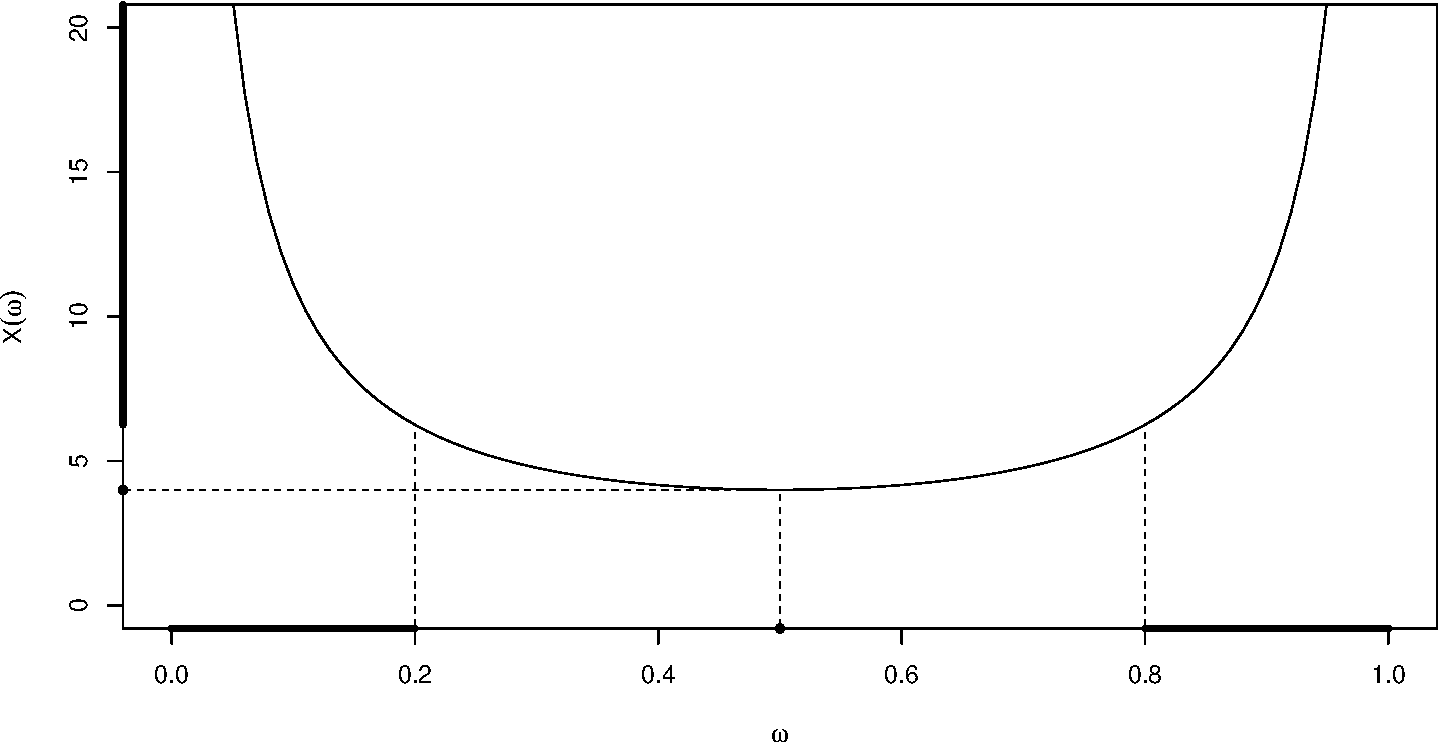
\includegraphics[width=0.7\linewidth,height=\textheight,keepaspectratio]{rvs_files/figure-pdf/unnamed-chunk-2-1.pdf}

}

\caption{Figure: 확률변수 \(X\)의 그림.}

\end{figure}%

\end{example}

\section{Radon-nikodym derivative}\label{radon-nikodym-derivative}

\begin{figure}[H]

{\centering 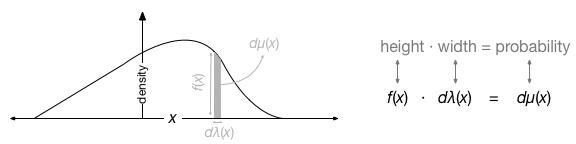
\includegraphics[width=1\linewidth,height=\textheight,keepaspectratio]{images/radon-nikodym.png}

}

\caption{Change of measures.}

\end{figure}%

확률측도는 volume element의 일반화라고 볼 수 있다.

\begin{itemize}
\item
  \(\mu(x)\): probability measure, interval이나 set of points들을
  인풋으로 받고 area/volume에 해당하는 확률(양수)을 아웃풋으로 주는
  함수다.
\item
  \(\lambda (x)\): reference measure. We often take \(\lambda (x)\) as
  the Lebesgue measure which is essentially just a uniform function over
  the sample space.
\end{itemize}

The reference measure \(\lambda (x)\) is essentially just a meter-stick
that allows us to express the probability measure as a simple function
\(f(x)\). That is, we represent the probability measure \(\mu(x)\) as
\(f(x)\) by comparing the probability measure to some specified
reference measure \(\lambda (x)\). This is essentially the intuition
that is given by the Radon-Nikodym derivative \[
f(x) = \frac{d\mu (x)}{d\lambda (x)}
\] or equivalently \[
\text{height = area / width.}
\] Note that we can also represent the same idea by \[
\mu (A) = \int_{A\in X} f(x) d\lambda (x),
\] where \(\mu(A)\) is the sum of the probability of events in the set
\(A\) which is itself a subset of the entire sample space \(X\). Note
that when \(A=X\) then the integral must equal \(1\) by definition of
probability.

라돈-니코딤 정리는 조건부 확률에 응용된다고 함.

\begin{definition}[Integrable Random
Variable]\protect\hypertarget{def-integrablerv}{}\label{def-integrablerv}

Gut (2014) 의 53쪽에 따르면, \(E|X|<\infty\)인 경우 random variable
\(X\)가 integrable 하다고 부른다.

\end{definition}

\begin{example}[]\protect\hypertarget{exm-lebesgueprob}{}\label{exm-lebesgueprob}

Given a probability measure \(P\) and sample space \(\Omega\), it is
true that \[
\int_{\Omega} dP = 1.
\] Because \[
\int_{\Omega} dP = P(\Omega) = 1.
\] More generally \[
\int_A dP = \int_{\Omega} 1_A dP = P(A), \quad{} A \in \mathcal{F}.
\]

\end{example}

\begin{definition}[\(\mathcal{L}^p\)]\protect\hypertarget{def-Lp}{}\label{def-Lp}

다음과 같은 확률공간 \((\Omega, \mathcal{F}, P)\)를 생각하자. \(p>1\)에
대해, 확률변수 \(X\)가 \(E|X|^p < \infty\)이면
\(X\in \mathcal{L}^p\)\index{$L^p$수렴}라고 하며 다음과 같은 놈
\(\|X_p\| = (E|X|^p)^{\frac{1}{p}}\)를 정의할 수 있다.

\end{definition}

\section{Distribution}\label{distribution}

\begin{itemize}
\item
  확률변수의 정의는 임의의 measurable subset of possible outcomes
  (points, bounded/unbounded intervals 등)에 measure (확률)를 부여할 수
  있어야 함
\item
  Semi-infinite interval \((-\infty, x]\) 또한 이러한 measurable
  subset이므로 \(\mathbb{R}\)에서 정의된 모든 확률변수는 CDF를 갖음
\item
  PDF는 CDF의 도함수 개념이므로 CDF가 미분가능해야 전역적으로 PDF도 존재
\end{itemize}

\section{Expectation}\label{expectation}

\begin{itemize}
\tightlist
\item
  \textbf{Expectation}: integral with respect to the probability measure
\end{itemize}

\begin{definition}[Expectation]\protect\hypertarget{def-expectation}{}\label{def-expectation}

~

\begin{itemize}
\item
  \((\Omega, \mathcal{A}, \mathbb{P})\): Probability space

  \begin{itemize}
  \tightlist
  \item
    \(\Omega\): set (sample space)
  \item
    \(\mathcal{A}\): \(\sigma\)-algebra on \(\Omega\)
  \item
    \(\mathbb{P}\): Probability measure
  \end{itemize}
\item
  \(X: \Omega \rightarrow \mathbb{R}\): Random variable (a measurable
  fct)
\item
  \textbf{Expectation}: The concept of integral of \(X\) w.r.t.
  \(\mathbb{P}\) \[
  E[X] \stackrel{\Delta}{=}\int_{\Omega} X(\omega) d\mathbb{P}[\omega]
  \]
\end{itemize}

\end{definition}

\begin{tcolorbox}[enhanced jigsaw, left=2mm, arc=.35mm, leftrule=.75mm, colback=white, title=\textcolor{quarto-callout-tip-color}{\faLightbulb}\hspace{0.5em}{Remark}, rightrule=.15mm, breakable, bottomrule=.15mm, coltitle=black, opacitybacktitle=0.6, opacityback=0, toptitle=1mm, titlerule=0mm, toprule=.15mm, colbacktitle=quarto-callout-tip-color!10!white, bottomtitle=1mm, colframe=quarto-callout-tip-color-frame]

\begin{itemize}
\tightlist
\item
  다음의 notation들은 모두 \(X\)의 기댓값을 의미

  \begin{itemize}
  \tightlist
  \item
    \(\int_{\Omega} X(\omega) d\mathbb{P}[\omega]\)
  \item
    \(\int_{\Omega} X d\mathbb{P}\) (적분하려는 변수가 분명한 경우 생략)
  \item
    \(\int_{\Omega} X(\omega) \mathbb{P}[d\omega]\)
  \end{itemize}
\end{itemize}

\end{tcolorbox}

\section{Cantor Random Variable}\label{cantor-random-variable}

\begin{itemize}
\item
  \href{https://en.wikipedia.org/wiki/Cantor_distribution}{Cantor
  distribution}: 누적분포함수가 Cantor function인 probability
  distribution
\item
  Cantor distribution은 PDF나 PMF가 존재하지 않음
\item
  동전던지기를 할 때, \(n\)번째 던지기에서 앞면이 나왔을 때
  \(\frac{2}{3^n}\)을 갖는 실험을 하면, 최종적으로 \(X\) 달러를 받는다고
  할 때, \(X\)는 확률변수이며 Cantor distribution의 예가 됨
\item
  특별히 \(\{\xi_n\}\)을 i.i.d. Bernoulli라 할 때 칸토르 확률변수
  \(X\)를 \(X=\sum_{n=1}^{\infty}\frac{2}{3^n}\xi_n\)과 같이 놓을 수
  있음 (위의 예제 참고)
\end{itemize}

\begin{itemize}
\tightlist
\item
  칸토를 집합을 \(C\)라 하고, \(X\in C\)라 할 때,
  \href{https://en.wikipedia.org/wiki/Cantor_set\#Measure_and_probability}{칸트로
  집합이 Lebesgue measure 0} 임을 알고 있으며, \(P(X\in C)=1>0\)이므로
  \(X\)는 \textbf{not absolutely continuous with respect to the Lebesgue
  measure}임
\end{itemize}

\begin{example}[Cantor distribution의 적률
계산]\protect\hypertarget{exm-cantorexp}{}\label{exm-cantorexp}

~

\begin{itemize}
\item
  PDF나 PMF가 존재하지 않더라도 Cantor distribution 같이 음이 아닌
  확률변수에서는 \(F(x) = P(X>x)\)를 계산할 수 있고, 이를 이용해 \[
  \begin{aligned}
  E(X) &= \int_0^{\infty} F(x) dx\\
  \text{Var} (X) &= \int_0^{\infty} 2x F(x) dx - \Big( \int_0^{\infty}F(x) dx \Big)^2
  \end{aligned}
  \] 와 같이 기댓값과 분산을 구할 수 있음
\item
  특별히 \(\{\xi_n\}\)을 i.i.d. Bernoulli라 할 때 칸토르 확률변수
  \(X\)를 \(X=\sum_{n=1}^{\infty}\frac{2}{3^n}\xi_n\)과 같이 놓을 수
  있고 (앞선 동전던지기 참고) \(E(\xi_n)=\frac{1}{2}\),
  \(\text{Var}(\xi_n) = \frac{1}{4}\)라는 점을 이용해 다음과 같이 구할
  수 있음 \[
  \begin{aligned}
  E(X) &= \sum_{n=1}^{\infty} E\Big( \frac{2}{3^n} \xi_n \Big)= \sum_{n=1}^{\infty}  \frac{2}{3^n} E(\xi_n)\\&= \sum_{n=1}^{\infty} \frac{2}{3^n }\cdot \frac{1}{2}= \sum_{n=1}^{\infty} \frac{1}{3^n} = \frac{1}{2}\\
  \text{Var}(X) &= \sum_{n=1}^{\infty} \text{Var}\Big( \frac{2}{3^n} \xi_n \Big)= \sum_{n=1}^{\infty}  \Big(\frac{2}{3^n}\Big)^2 \text{Var}(\xi_n)\\&= \sum_{n=1}^{\infty} \frac{4}{9^n }\cdot \frac{1}{4}= \sum_{n=1}^{\infty} \frac{1}{9^n} = \frac{1}{8}.
  \end{aligned}
  \]
\end{itemize}

\end{example}

\begin{example}[\(g(X)\)가 불연속이나 \(E[g(X)]\)는 연속인
예]\protect\hypertarget{exm-expcont}{}\label{exm-expcont}

\(X\sim \text{Exp}(1)\), \(g(X)\)를 \[
g(X) =
\begin{cases}
0, & \text{if }X=0\\
1, & \text{if }X\in (0,3)\\
1+0.4 (X-3), & \text{if }X \geq 3
\end{cases}
\] 이라고 하자. 이때 \[
g(x) = 0I_{0}(x) + 1I_{(0,3)}(x) + \{ 1+0.4 (x-3) \} I_{(0,3)^c}(x)
\] 이다. \[
E[g(X)] = E[0I_{0}(X)] + E[1I_{(0,3)}(X)] + E[\{1+0.4(X-3)\}I_{(0,3)^c}(X)]
\] 인데, 첫 번째 항은 0이고 \[
E[1I_{(0,3)}(X)]  = \int 1 1I_{(0,3)}(x)\exp\{-x\}dx = \int_0^3 \exp \{-x\} dx = 1-\exp \{-3\},
\] \[
\begin{aligned}
E[\{1+0.4(X-3)\}I_{(0,3)^c}(X)] &= \int \{1+0.4(x-3) \} I_{(0,3)^c}(x)\exp\{-x\}dx\\
&= \int_3^{\infty}\{1+0.4(x-3) \}\exp \{-x\}dx\\
&= \exp \{-3\}+0.4 \int_0^{\infty} x\exp \{-(x+3)\}dx\\
&= \exp \{-3\}+0.4\exp \{-3\} \int_0^{\infty} x \exp \{-x\}dx\\
&= \exp \{-3\} + 0.4 \exp \{-3\}
\end{aligned}
\] 즉 \(E[g(X)] = 1+0.4\exp\{-3\}\)이다.

\end{example}

\section{Borel-Cantelli Lemmas}\label{borel-cantelli-lemmas}

\begin{itemize}
\tightlist
\item
  Almost sure convergence Definition~\ref{def-sconv} 와 관련된 툴
\end{itemize}

\begin{theorem}[The first Borel-Cantelli
lemma]\protect\hypertarget{thm-firstborelcantelli}{}\label{thm-firstborelcantelli}

Let \(\{A_n, n \geq 1\}\) be arbitrary events. Then \[
\sum_{n=1}^{\infty}P(A_n) < \infty \Longrightarrow P(A_n \text{ i.o.})=0.
\]

\end{theorem}

\begin{tcolorbox}[enhanced jigsaw, left=2mm, arc=.35mm, leftrule=.75mm, colback=white, title=\textcolor{quarto-callout-note-color}{\faInfo}\hspace{0.5em}{Proof}, rightrule=.15mm, breakable, bottomrule=.15mm, coltitle=black, opacitybacktitle=0.6, opacityback=0, toptitle=1mm, titlerule=0mm, toprule=.15mm, colbacktitle=quarto-callout-note-color!10!white, bottomtitle=1mm, colframe=quarto-callout-note-color-frame]

\[
\begin{aligned}
P(A_n \text{ i.o.}) &= P(\lim\sup_{n\rightarrow\infty}A_n) = P \Big (\bigcap_{n=1}^{\infty}\bigcup_{m=n}^{\infty}A_m\Big)\\
&\leq P\Big( \bigcup_{m=n}^{\infty}A_m \Big) \leq \sum_{m=n}^{\infty}P(A_m) \stackrel{n\rightarrow\infty}{\longrightarrow}0.
\end{aligned}
\]

\end{tcolorbox}

\begin{tcolorbox}[enhanced jigsaw, left=2mm, arc=.35mm, leftrule=.75mm, colback=white, title=\textcolor{quarto-callout-tip-color}{\faLightbulb}\hspace{0.5em}{Remark}, rightrule=.15mm, breakable, bottomrule=.15mm, coltitle=black, opacitybacktitle=0.6, opacityback=0, toptitle=1mm, titlerule=0mm, toprule=.15mm, colbacktitle=quarto-callout-tip-color!10!white, bottomtitle=1mm, colframe=quarto-callout-tip-color-frame]

\begin{itemize}
\tightlist
\item
  The first Borel-Cantelli lemma의 역은 성립하지 않는다. 그러나 독립
  조건을 넣으면 다음과 같은 second Borel-Cantelli lemma를 얻을 수 있다.
\end{itemize}

\end{tcolorbox}

\begin{theorem}[The second Borel-Cantelli
lemma]\protect\hypertarget{thm-secondborelcantelli}{}\label{thm-secondborelcantelli}

Let \(\{A_n, n \geq 1\}\) be \textbf{independent} events. Then \[
\sum_{n=1}^{\infty}P(A_n) = \infty \Longrightarrow P(A_n \text{ i.o.})=1.
\]

\end{theorem}

\begin{tcolorbox}[enhanced jigsaw, left=2mm, arc=.35mm, leftrule=.75mm, colback=white, title=\textcolor{quarto-callout-note-color}{\faInfo}\hspace{0.5em}{Proof}, rightrule=.15mm, breakable, bottomrule=.15mm, coltitle=black, opacitybacktitle=0.6, opacityback=0, toptitle=1mm, titlerule=0mm, toprule=.15mm, colbacktitle=quarto-callout-note-color!10!white, bottomtitle=1mm, colframe=quarto-callout-note-color-frame]

By independence \[
\begin{aligned}
P(A_n \text{ i.o.}) &= P(\lim\sup_{n\rightarrow\infty}A_n) = P \Big (\bigcap_{n=1}^{\infty}\bigcup_{m=n}^{\infty}A_m\Big)=1-P \Big (\bigcup_{n=1}^{\infty}\bigcap_{m=n}^{\infty}A_m^c\Big)\\
&=1 - \lim_{n\rightarrow\infty}P\Big( \bigcap_{m=n}^{\infty}A_m^c\Big) = 1-\lim_{n\rightarrow\infty}\prod_{m=n}^{\infty}P(A_m^c)\\
&=1 - \lim_{n\rightarrow\infty}\prod_{m=n}^{\infty}(1-P(A_m)) = 1-0 = 1.
\end{aligned}
\]

\end{tcolorbox}

\chapter{Inequalities}\label{sec-ineq}

\section{왜 concentration inequality가
필요한가?}\label{uxc65c-concentration-inequalityuxac00-uxd544uxc694uxd55cuxac00}

\begin{itemize}
\tightlist
\item
  출처:
  \href{https://gclinderman.github.io/blog/probability/2018/01/07/concentration-inequalities.html}{Concentration
  Inequalities}
\end{itemize}

\begin{itemize}
\item
  \href{https://www.math.uci.edu/~rvershyn/papers/HDP-book/HDP-book.html}{High-Dimensional
  Probability} 책에 있는 동전 던지기 예제 생각
\item
  \(i\)번째 동전던지기: 앞면이 나오면 1, 뒷면이 나오면 0인 Bernoulli
  random variable로 간주 가능
\item
  \(N\)번 던졌을 때 나온 앞면의 수: \(S_N = \sum_i X_i\)
\item
  de Moivre-Laplace theorem (Binomial의 CLT) \[
  Z_N \stackrel{D}{\rightarrow}\mathcal{N}(0,1)
  \] 이때 \[
  Z_N  = \frac{S_N - N_p}{\sqrt{Np (1-p)}}
  \]
\end{itemize}

\begin{figure}[H]

{\centering 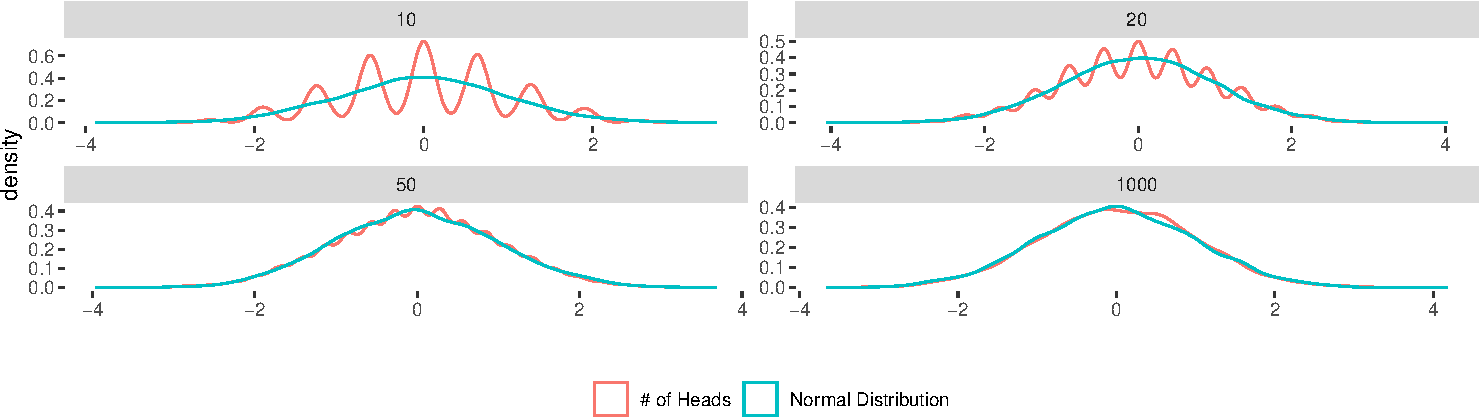
\includegraphics[width=0.7\linewidth,height=\textheight,keepaspectratio]{ineq_files/figure-pdf/unnamed-chunk-2-1.pdf}

}

\caption{Figure: CLT 묘사.}

\end{figure}%

\textbf{Q}. \(N\)번 시행 시 \(\frac{3}{4}\)이상 앞면이 나올 확률을
구하고 싶다.

\begin{itemize}
\item
  Gaussian density는 exponential decay하는데, \(Z_N\)이 분포수렴하는
  속도는 훨씬 느림
\item
  CLT의 quantitative version인 Berry-Essen CLT를 보면 \[
  |P\{Z_n \geq t\} - P\{Z \geq t\} | \leq \frac{C}{\sqrt{N}}
  \] 이때 \(C\)는 상수이며, convergence의 order가
  \(\frac{1}{\sqrt{N}}\)임을 (아래 그림에 녹색으로 표시) 확인 가능
\end{itemize}

\begin{figure}[H]

{\centering 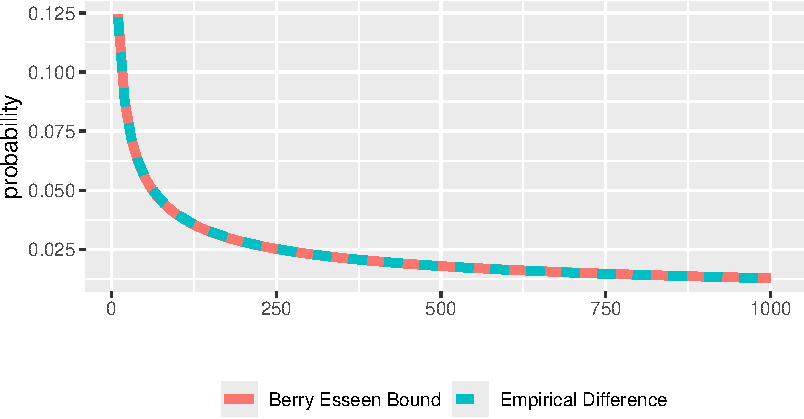
\includegraphics[width=0.7\linewidth,height=\textheight,keepaspectratio]{ineq_files/figure-pdf/unnamed-chunk-3-1.pdf}

}

\caption{Figure: Berry-Essen bound와 empirical difference.}

\end{figure}%

\section{Markov inequality}\label{markov-inequality}

\begin{theorem}[Markov
inequality]\protect\hypertarget{thm-markovineq}{}\label{thm-markovineq}

음이 아는 확률변수 \(X\)에 대해 \[
P\{ X\geq t\} \leq \frac{E[X]}{t}
\]

\end{theorem}

\begin{tcolorbox}[enhanced jigsaw, left=2mm, arc=.35mm, leftrule=.75mm, colback=white, title=\textcolor{quarto-callout-note-color}{\faInfo}\hspace{0.5em}{Proof}, rightrule=.15mm, breakable, bottomrule=.15mm, coltitle=black, opacitybacktitle=0.6, opacityback=0, toptitle=1mm, titlerule=0mm, toprule=.15mm, colbacktitle=quarto-callout-note-color!10!white, bottomtitle=1mm, colframe=quarto-callout-note-color-frame]

확률공간 \((\Omega, \Sigma, P)\)을 생각하자. \[
EX = \int X dP \geq \int_{\{X\geq t\}} X dP \geq t \int_{\{X\geq t \}}dP \geq t\cdot P\{ X\geq t\}
\]

\end{tcolorbox}

\begin{tcolorbox}[enhanced jigsaw, left=2mm, arc=.35mm, leftrule=.75mm, colback=white, title=\textcolor{quarto-callout-tip-color}{\faLightbulb}\hspace{0.5em}{Remark}, rightrule=.15mm, breakable, bottomrule=.15mm, coltitle=black, opacitybacktitle=0.6, opacityback=0, toptitle=1mm, titlerule=0mm, toprule=.15mm, colbacktitle=quarto-callout-tip-color!10!white, bottomtitle=1mm, colframe=quarto-callout-tip-color-frame]

\begin{itemize}
\item
  마르코프 bound는 매우 약한 (즉 true probabilty로의 수렴이 느린) bound
\item
  그러나 \(X\)에 대한 제약조건이 없음 (기댓값 계산 필요, 음이 아닌
  확률변수)
\end{itemize}

\end{tcolorbox}

\section{Chebyshev inequality}\label{chebyshev-inequality}

\begin{theorem}[Chebyshev
inequality]\protect\hypertarget{thm-chevyshevineq}{}\label{thm-chevyshevineq}

어떤 확률변수 \(X\)에 대해 \[
P\{|X-E(X)|\geq t \}\leq \frac{\text{Var}(X)}{t^2}
\]

\end{theorem}

\begin{tcolorbox}[enhanced jigsaw, left=2mm, arc=.35mm, leftrule=.75mm, colback=white, title=\textcolor{quarto-callout-note-color}{\faInfo}\hspace{0.5em}{Proof}, rightrule=.15mm, breakable, bottomrule=.15mm, coltitle=black, opacitybacktitle=0.6, opacityback=0, toptitle=1mm, titlerule=0mm, toprule=.15mm, colbacktitle=quarto-callout-note-color!10!white, bottomtitle=1mm, colframe=quarto-callout-note-color-frame]

\(|X-E(X)|\geq t\)를 제곱한 후 마르코프 부등식을 적용 \[
P\{ |X-E(X)|^2 \geq t^2\} \leq \frac{E[(X-E(X))]^2}{t^2} = \frac{\text{Var}(X)}{t^2}
\]

\end{tcolorbox}

\begin{tcolorbox}[enhanced jigsaw, left=2mm, arc=.35mm, leftrule=.75mm, colback=white, title=\textcolor{quarto-callout-tip-color}{\faLightbulb}\hspace{0.5em}{Remark}, rightrule=.15mm, breakable, bottomrule=.15mm, coltitle=black, opacitybacktitle=0.6, opacityback=0, toptitle=1mm, titlerule=0mm, toprule=.15mm, colbacktitle=quarto-callout-tip-color!10!white, bottomtitle=1mm, colframe=quarto-callout-tip-color-frame]

\begin{itemize}
\tightlist
\item
  체비세프 부등식을 쓰려면 분산이 정의되어야 함
\end{itemize}

\end{tcolorbox}

\section{Hoeffding's Inequality}\label{hoeffdings-inequality}

\begin{itemize}
\item
  (드디어) \(\sum_i X_i\)에 대한 exponential bound를 줌
\item
  그러나 독립 가정이 필요
\item
  단순한 케이스로 먼저 \(X_1, \ldots, X_N\)이 symmetric Bernoulli라고
  하자. 이는 즉 반반의 확률로 1 또는 -1을 갖는 확률변수
\end{itemize}

\begin{theorem}[Symmetric Bernoulli에서의 Hoeffding's
inequality]\protect\hypertarget{thm-hoeffdingbernoulli}{}\label{thm-hoeffdingbernoulli}

\(X_1, \ldots, X_N\)이 symmetric Bernoulli 확률변수라고 하자. 어떤
\(t\geq 0\)에 대해 \(a \in \mathbb{R}^n\)이 존재해 \[
P\{ \sum_{i=1}^N a_i X_i \geq t \} \leq \exp \Big( - \frac{t^2}{2\|a\|^2} \Big)
\]

\end{theorem}

\begin{tcolorbox}[enhanced jigsaw, left=2mm, arc=.35mm, leftrule=.75mm, colback=white, title=\textcolor{quarto-callout-note-color}{\faInfo}\hspace{0.5em}{Proof}, rightrule=.15mm, breakable, bottomrule=.15mm, coltitle=black, opacitybacktitle=0.6, opacityback=0, toptitle=1mm, titlerule=0mm, toprule=.15mm, colbacktitle=quarto-callout-note-color!10!white, bottomtitle=1mm, colframe=quarto-callout-note-color-frame]

마르코프 부등식을 적용하면 다음과 같다. \[
P\{ \sum_{i=1}^N a_i X_i \geq t \} = P \{ \exp (\lambda \sum_{i=1}^N a_i X_i) \geq e^{\lambda t} \} \leq e^{-\lambda t}E\{ \exp (\lambda \sum_{i=1}^N a_i X_i) \}
\] 독립성에 의해 다음과 같다. \[
E\{ \exp (\lambda \sum_{i=1}^N a_i X_i) \} = E \{ \prod_{i=1}^N \exp (\lambda a_i X_i)  \} = \prod_{i=1}^N E\{ \exp (\lambda a_i X_i)\}
\] \(X_i\)를 \(1/2\)의 확률로 -1과 1을 갖는 확률변수라고 제한했으므로,
위의 기댓값을 쉽게 구할 수 있다. \[
E\{ \exp (\lambda a_i X_i)\} = \frac{e^{\lambda a_i }+ e^{-\lambda a_i}}{2}\leq e^{\lambda^2 a_i^2 / 2}
\] 지수함수의 테일러 급수 전개를 이용하면 \[
e^{x}=\sum_{k=0}^{\infty}\frac{x^k}{k!},\quad{} \frac{e^{x}+e^{-x}}{2} =\sum_{k=0}^{\infty}\frac{x^{2k}}{(2k)!}, \quad{} e^{x^2/2}=\sum_{k=0}^{\infty}\frac{x^{2k}}{2^k k!},\quad{} \Longrightarrow\quad{} \frac{e^{x}+e^{-x}}{2} \leq e^{x^2/2}.
\] \(\|a\|^2=1\)이라 두고 위의 결과를 대입해보자. \[
P\{ \sum_{i=1}^N a_i X_i \geq t \} \leq e^{-\lambda t}(\prod_{i=1}^N e^{\lambda^2 a_i^2/2})\leq e^{-\lambda t}(e^{\lambda^2 \sum_{i=1}^N a_i^2/2}) = e^{-\lambda t}(e^{\lambda^2/2}) = e^{\lambda^2/2 - \lambda t}.
\] 위의 부등식은 모든 \(\lambda\)에 대해 성립하고, \(\lambda=t\)일 때
최소화된다. 따라서 \[
P\{ \sum_{i=1}^N a_i X_i \geq t \} \leq e^{-t^2/2}.
\] 따라서, homogeneity에 의해 \(\|a\|=1\)을 가정하면 다음과 같다. \[
P \{ \sum_{i=1}^N \frac{a_i}{\| a\|}X_i \geq \frac{t}{\|a\|} \} \leq e^{-\frac{t^2}{2\|a\|^2}}.
\]

\end{tcolorbox}

\(X_i\)가 1 또는 0을 갖는 베르누이 확률변수라고 할 때,
\(Y_i = 2(X_i - \frac{1}{2})\)로 놓으면 \(Y_i\)는 symmetric Bernoulli
확률변수임 \[
P\{ \sum_i X_i > t\} = P \{ \sum_i (\frac{Y_i}{2}+ \frac{1}{2}) > t \} = P\{\sum_i Y_i > 2t - N \} \leq \exp (-\frac{(2t-N)^2}{2N})
\] 여기서 \(a=\begin{bmatrix} 1,1,\ldots, 1 \end{bmatrix}\)로 두면
\(\|a\|_2^2=N\)이 된다. 따라서 \[
P\{\sum_i X_i > \frac{3N}{4} \}\leq \exp (- \frac{(\frac{3N}{2}-N)^2}{2N}) = \exp (-\frac{N}{8})
\]

\begin{figure}[H]

{\centering 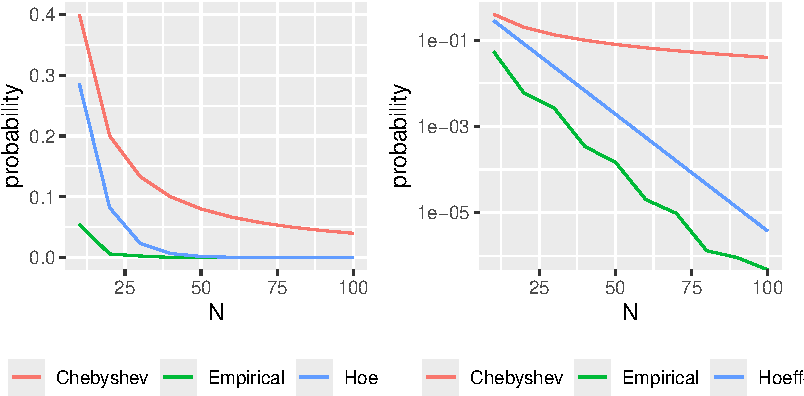
\includegraphics[width=0.7\linewidth,height=\textheight,keepaspectratio]{ineq_files/figure-pdf/unnamed-chunk-4-1.pdf}

}

\caption{Figure: Chebyshev와 Hoeffding bound의 비교.}

\end{figure}%

\begin{theorem}[Hoeffding's
inequality]\protect\hypertarget{thm-hoeffdingineq}{}\label{thm-hoeffdingineq}

\(X_1, \ldots, X_N\)이 독립인 확률변수이고, \(X_i \in [m_i, M_i]\)
almost surely라고 하자. 그러면 어떤 \(t>0\)에 대해 \[
P \{\sum_{i=1}^N (X_i - E(X_i))\geq t \} \leq \exp (- \frac{2t^2}{\sum_{i=1}^N (M_i - m_i)^2})
\]

\end{theorem}

\begin{tcolorbox}[enhanced jigsaw, left=2mm, arc=.35mm, leftrule=.75mm, colback=white, title=\textcolor{quarto-callout-note-color}{\faInfo}\hspace{0.5em}{Proof}, rightrule=.15mm, breakable, bottomrule=.15mm, coltitle=black, opacitybacktitle=0.6, opacityback=0, toptitle=1mm, titlerule=0mm, toprule=.15mm, colbacktitle=quarto-callout-note-color!10!white, bottomtitle=1mm, colframe=quarto-callout-note-color-frame]

앞에서처럼 \(\lambda\)를 곱하고 제곱근을 취한 다음 마르코프 부등식을
이용한다 \[
\begin{align*}
P\{\sum (X_i - E(X_i)) \geq t \} &= P \{\exp (\lambda \sum (X_i - E(X_i)))\geq e^{\lambda t} \}\\
&\leq E \{\exp (\lambda \sum (X_i - E(X_i)))\} e^{-\lambda t}\\
&= \prod_i E\{\exp (\lambda (X_i - E(X_i))) \}e^{-\lambda t}.
\end{align*}
\] 그러면 기댓값의 bound만 찾아주면 된다. 여기서는 \(X_i\)와 독립인
copy인 \(X_i'\)를 생각하는 \textbf{symmetrization} 기법을 이용한다. \[
\begin{align*}
E\{\exp (\lambda \sum (X_i - E(X_i)) ) \} &= E\{\exp (\lambda \sum (X_i - E(X_i')) ) \} \\
&= E_{X_i} \{ \exp (E_{X_i'} \lambda \sum (X_i - X_i')) \}\\
&\leq E_{X_i} E_{X_i'} \{ \exp (\lambda \sum (X_i - X_i')) \}\\
&= E\{ \exp (\lambda \sum (X_i - X_i')) \}.
\end{align*}
\] 여기서 exponential이 convex이므로 Jensen의 부등식을 적용하였다.
여기서 \(X_i - X_i'\)는 0 근처에서 symmetric이고 이것의 분포는
\(S(X_i - X_i')\)와 같다. 이때 \(S\)는 -1, 1을 동일한 확률로 갖는
\textbf{Rademacher variable}이다. \[
\begin{align*}
E\{\exp (\lambda \sum (X_i - E(X_i)) ) \} &\leq E_{X_i,X_i'} \{ E_S \exp (\lambda \sum S(X_i - X_i')) \}\\
&\leq E_{X_i,X_i'} \{ \exp (\lambda^2 (X_i - X_i')^2/2) \}\\
&\leq \exp (\lambda^2 (M_i - m_i)^2/2).
\end{align*}
\] 이때 첫 번째 부등식은 exponential의 테일러 전개를, 두 번째 부등식은
\(X_i\)의 boundedness를 이용하였다. \[
\begin{align*}
P\{\sum (X_i - E(X_i)) \geq t \} &=  \prod_i E\{\exp (\lambda (X_i - E(X_i))) \}e^{-\lambda t}\\
&= \prod_i \exp (\lambda^2 (M_i - m_i)^2/2)e^{-\lambda t}\\
&= \exp (\lambda^2 \sum_i (M_i - m_i)^2/2 -\lambda t)\\
&\leq \exp (\frac{2t^2}{\sum_i (M_i -m_i)^2}).
\end{align*}
\] 여기서 마지막 부등식은 exponent를 최소화하는 \(\lambda\)를 잡았다.

\end{tcolorbox}

\section{Chernoff Bounds}\label{chernoff-bounds}

\begin{itemize}
\item
  베르누이 확률변수에 대한 Hoeffding bound는 \(p=0.5\)일 때에는 잘
  작동하지만, 작거나 큰 \(p\)에 대해서는 잘 작동하지 않음
\item
  \(X_i \sim \text{Bernoulli}(p)\)라고 하고
  \(S_N = \sum_{i=1}^N X_i\)라고 두자. 그리고 Hoeffding의 부등식을
  이용하여 \(S_N > 10pN\)의 bound를 구해보자. \[
  P \{ \sum_i X_i > 10pN \} = P\{ \sum_i X_i - pN > 9pN \}\leq \exp (-\frac{2(9pN)^2}{N}) = \exp (-182p^2 N).
  \] 식을 보면 Binomial random variable이 평균보다 9배 클 확률의 bound를
  계산함
\end{itemize}

\begin{theorem}[Chernoff
inequality]\protect\hypertarget{thm-chernoffineq}{}\label{thm-chernoffineq}

\(X_1, \ldots, X_N\)이 모수 \(p_i\)를 갖는 독립인 베르누이 확률변수라
하자. \(S_N = \sum_i X_i\)이고 \(\mu = E(S_N)\)이라고 하자. 그러면
\(t>\mu\)에 대해 \[
P \{ S_N \geq t \} \leq \exp (-\mu) \Big( \frac{e\mu}{t} \Big)^t.
\]

\end{theorem}

\begin{tcolorbox}[enhanced jigsaw, left=2mm, arc=.35mm, leftrule=.75mm, colback=white, title=\textcolor{quarto-callout-note-color}{\faInfo}\hspace{0.5em}{Proof}, rightrule=.15mm, breakable, bottomrule=.15mm, coltitle=black, opacitybacktitle=0.6, opacityback=0, toptitle=1mm, titlerule=0mm, toprule=.15mm, colbacktitle=quarto-callout-note-color!10!white, bottomtitle=1mm, colframe=quarto-callout-note-color-frame]

다시 \(\lambda\)를 곱하고 마르코프 부등식을 적용하자. \[
P\{ S_N \geq t \} \leq E\{ \exp (\lambda \sum_{i} X_i) \}e^{-\lambda t} = \prod_i E\{ \exp (\lambda X_i) \}e^{-\lambda t}.
\] \(1+x \leq e^{x}\)라는 부등식을 이용하면 다음과 같다. \[
P\{ S_N \geq t \} \leq  e^{\lambda}p_i + (1-p_i) = 1 + (e^{\lambda} - 1)p_i \leq \exp (p_i (e^\lambda - 1)).
\] 이것을 정리하면 다음과 같다. \[
\begin{align*}
P\{ S_N \geq t \} &\leq \prod_i \exp (p_i (e^\lambda -1))e^{-\lambda t}\\
&\leq \exp \Big( (e^\lambda - 1)\sum_i p_i \Big) e^{-\lambda t}\\
&\leq \exp ((e^{\lambda}-1)\mu) e^{-\lambda t}.
\end{align*}
\] 여기서 \(\lambda\)를 고를 수 있는데, \(\lambda = \log (t/mu)\)로
잡으면 다음과 같다. \[
\begin{align*}
P\{ S_N \geq t \} &\leq \exp \Big( (\frac{t}{\mu}-1)\mu \Big) \Big( \frac{\mu}{t} \Big)^t\\
&= \exp (t-\mu) \Big( \frac{\mu}{t} \Big)^t\\
&=\exp (-\mu) \Big( \frac{e\mu}{t} \Big)^t.
\end{align*}
\]

\end{tcolorbox}

\begin{itemize}
\tightlist
\item
  다시 앞 예제에 Chernoff 부등식을 적용하면 \[
  P \{\sum_i X_i > 10pN \} \leq \exp (-p N) \Big( \frac{epN}{10pN}\Big)^{10pN} = \exp (-p N) \Big( \frac{e}{10}\Big)^{10pN}.
  \]
\end{itemize}

\begin{figure}[H]

{\centering 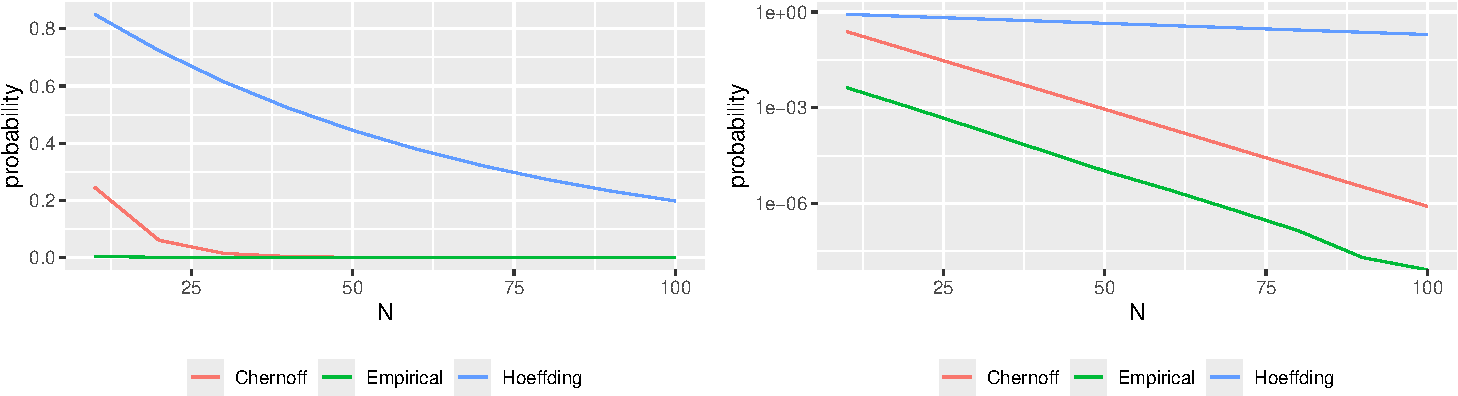
\includegraphics[width=0.7\linewidth,height=\textheight,keepaspectratio]{ineq_files/figure-pdf/unnamed-chunk-5-1.pdf}

}

\caption{Figure: Hoeffding과 Chernoff bound의 비교.}

\end{figure}%

\section{Gaussian tails and MGF}\label{gaussian-tails-and-mgf}

\begin{itemize}
\item
  출처:
  \href{https://ocw.mit.edu/courses/18-s997-high-dimensional-statistics-spring-2015/a69e2f53bb2eeb9464520f3027fc61e6_MIT18_S997S15_Chapter1.pdf}{High-Dimensional
  Statistics Lecture Notes}
\item
  \(X\)가 Gaussian일 때 pdf \[
  p(x) = \frac{1}{\sqrt{2\pi \sigma^2}} \exp \Big( - \frac{(x-\mu)^2}{2\sigma^2} \Big), \quad{} x \in \mathbb{R}
  \]
\item
  특별히 standard normal의 pdf를 다음과 같이 두기로 함 \[
  \phi (x) = \frac{1}{\sqrt{2\pi}}\exp \Big( -\frac{x^2}{2} \Big)
  \]
\item
  Bounded support: \(P(|X-\mu|\leq 3\sigma)\) 등의 확률 구할 때 사용
\end{itemize}

\begin{proposition}[Mills
inequality]\protect\hypertarget{prp-millsineq}{}\label{prp-millsineq}

Gaussian density tail의 decay 속도를 알려줌

\begin{itemize}
\item
  \(X\sim \mathcal{N}(\mu, \sigma^2)\)일 때 \(t>0\)에 대해
  \begin{equation}\phantomsection\label{eq-concentgaussian}{
  P(|X-\mu | >t) \leq \sqrt{\frac{2}{\pi}}\frac{e^{-\frac{t^2}{2\sigma^2}}}{t}.
  }\end{equation}
\item
  특별히 \(X\sim \mathcal{N}(0,1)\)일 때 \(t>0\)에 대해 \[
  P(|X | >t) \leq \frac{2\phi (t)}{t}
  \]
\item
  \(\phi(x)\)를 이용해 특별히 \(X\sim \mathcal{N}(0,\sigma^2)\)일 때
  \(t>0\)에 대해 \[
  P(|X | >t) \leq 2\frac{\sigma}{t}\phi \Big(\frac{t}{\sigma} \Big) = \sqrt{\frac{2}{\pi}}\frac{\sigma}{t}\exp \Big( - \frac{t^2}{2\sigma^2}\Big).
  \]
\end{itemize}

\end{proposition}

\begin{tcolorbox}[enhanced jigsaw, left=2mm, arc=.35mm, leftrule=.75mm, colback=white, title=\textcolor{quarto-callout-note-color}{\faInfo}\hspace{0.5em}{Proof}, rightrule=.15mm, breakable, bottomrule=.15mm, coltitle=black, opacitybacktitle=0.6, opacityback=0, toptitle=1mm, titlerule=0mm, toprule=.15mm, colbacktitle=quarto-callout-note-color!10!white, bottomtitle=1mm, colframe=quarto-callout-note-color-frame]

\begin{itemize}
\item
  우선 unit variance일 경우, \(X\)가 symmetric around origin임을
  이용하여 \[
  P(|X|>t) = 2P(X>t).
  \] 마르코프 부등식의 증명과 비슷하게 \[
  \begin{align*}
  t\cdot P(|X|>t) &= t \int_t^{\infty} \phi (x) dx\\
  &\leq \int_t^{\infty} x \phi(x)dx\\
  &= \int_t^{\infty} \frac{1}{\sqrt{2\pi}}x \exp \Big( -\frac{x^2}{2}\Big) dx\\
  &= \frac{1}{\sqrt{2\pi}}\int_{t}^{\infty}-\frac{\partial}{\partial x}\exp \Big( -\frac{x^2}{2}\Big)dx\\
  &= \frac{1}{\sqrt{2\pi}}\exp \Big( - \frac{t^2}{2} \Big).
  \end{align*}
  \]
\item
  일반적인 케이스의 경우 \(X/\sigma \sim \mathcal{N}(0,1)\)이고 \[
  P(|X|>t) = P \Big( \Big\vert\frac{X}{\sigma}\Big\vert > \frac{t}{\sigma} \Big)
  \] 로부터 유도됨
\end{itemize}

\end{tcolorbox}

\begin{proposition}[Gaussian의 concentration
inequality]\protect\hypertarget{prp-concentrationineqgaussian}{}\label{prp-concentrationineqgaussian}

~

\begin{itemize}
\tightlist
\item
  Mills inequality의 application
\end{itemize}

\(X_i \sim\mathcal{N}(0,\sigma^2)\) (이때 확률변수들은 독립이 아니어도
됨)일 때, \(t>0\)에 대해 \[
P(\max_{1\leq i \leq n} |X_i | >t) \leq 2n \frac{\sigma}{t}\phi \Big( \frac{t}{\sigma} \Big).
\]

\end{proposition}

\begin{tcolorbox}[enhanced jigsaw, left=2mm, arc=.35mm, leftrule=.75mm, colback=white, title=\textcolor{quarto-callout-note-color}{\faInfo}\hspace{0.5em}{Proof}, rightrule=.15mm, breakable, bottomrule=.15mm, coltitle=black, opacitybacktitle=0.6, opacityback=0, toptitle=1mm, titlerule=0mm, toprule=.15mm, colbacktitle=quarto-callout-note-color!10!white, bottomtitle=1mm, colframe=quarto-callout-note-color-frame]

Mills 부등식에 union bound를 쓰면 된다고 함

\end{tcolorbox}

\begin{proposition}[Max of Gaussian random variables의 upper
bound]\protect\hypertarget{prp-maxgaussianbound}{}\label{prp-maxgaussianbound}

~

\begin{itemize}
\tightlist
\item
  Mills inequality의 application, lower bound도 같은 rate로 유도 가능
\end{itemize}

\(X_i \sim\mathcal{N}(0,\sigma^2)\) (이때 확률변수들은 독립이 아니어도
됨)일 때, \[
E[\max_{1\leq i \leq n}X_i] \leq \sigma \sqrt{2\log n}
\] 이고 \[
E[\max_{1\leq i \leq n} |X_i|] \leq \sigma \sqrt{2\log 2n}
\]

\end{proposition}

\begin{tcolorbox}[enhanced jigsaw, left=2mm, arc=.35mm, leftrule=.75mm, colback=white, title=\textcolor{quarto-callout-note-color}{\faInfo}\hspace{0.5em}{Proof}, rightrule=.15mm, breakable, bottomrule=.15mm, coltitle=black, opacitybacktitle=0.6, opacityback=0, toptitle=1mm, titlerule=0mm, toprule=.15mm, colbacktitle=quarto-callout-note-color!10!white, bottomtitle=1mm, colframe=quarto-callout-note-color-frame]

\begin{itemize}
\tightlist
\item
  \(s>0\)에 대해 \[
  \begin{align*}
  E[\max_{1\leq i \leq n}X_i] &= \frac{1}{s}E[\log (\exp (s \max_{1\leq i \leq n} X_i))]\\
  &\stackrel{(a)}{\leq} \frac{1}{s} \log (E[\exp (s\max_{1\leq i \leq n}X_i)])\\
  &\stackrel{(b)}{=} \frac{1}{s}\log(E[\max_{1\leq i \leq n}\exp (sX_i)])\\
  &\stackrel{(c)}{\leq} \frac{1}{s}\log (\sum_{i=1}^n E[\exp (s X_i)])\\
  &\stackrel{(d)}{=}  \log \Big(\sum_{i=1}^n \exp \Big( \frac{s^2\sigma^2}{2} \Big) \Big)\\
  &= \frac{\log n}{s} + \frac{s^2 \sigma^2}{2}.
  \end{align*}
  \] 여기서

  \begin{itemize}
  \tightlist
  \item
    (a): Jensen 부등식
  \item
    (b): \(\exp (\cdot)\) 함수의 monotonicity
  \item
    (c): \(\max\)의 정의로부터
  \item
    (d): Gaussian r.v.의 MGF로부터
  \end{itemize}
\end{itemize}

\(s=\sqrt{2\log n}/\sigma\)로 놓아 upper bound를 minimize한다고 함

\end{tcolorbox}

\section{Sub-Gaussian}\label{sub-gaussian}

\begin{itemize}
\item
  출처:
  \href{https://gclinderman.github.io/blog/probability/2018/01/07/concentration-inequalities.html}{Concentration
  Inequalities}
\item
  앞서 Chernoff appraoch로 얻어지는 tail bound의 form은 MGF의 growth
  rate에 depend됨을 암
\item
  따라서 tail bound study에서는 확률변수들을 MGF에 따라 분류하는 것이
  자연스러운 생각
\item
  또한 Proposition~\ref{prp-maxgaussianbound} 의 증명을 보면, (d)를
  제외한 나머지 부분에서는 Gaussian의 성질이 쓰이지 않고 있음. 즉
  \(E[\exp (s X_i)]\leq \exp ( \frac{1}{2}s^2 \sigma^2)\)을 만족하는
  확률변수 \(X_i\)들에 대해서는 Proposition~\ref{prp-maxgaussianbound}
  의 결과가 성립할 것임
\end{itemize}

\begin{definition}[Sub-Gaussian]\protect\hypertarget{def-subgaussian}{}\label{def-subgaussian}

어떤 확률변수 \(X\in \mathbb{R}\)이 \(E(X)=0\)이고 이것의 MGF가 \[
E[\exp (sX)] \leq \exp \Big( \frac{\sigma^2 s^2}{2} \Big), \forall s \in \mathbb{R}
\] 일 때 \(X \sim \text{subG}(\sigma^2)\)이라고 한다.

\end{definition}

\begin{tcolorbox}[enhanced jigsaw, left=2mm, arc=.35mm, leftrule=.75mm, colback=white, title=\textcolor{quarto-callout-tip-color}{\faLightbulb}\hspace{0.5em}{Remark}, rightrule=.15mm, breakable, bottomrule=.15mm, coltitle=black, opacitybacktitle=0.6, opacityback=0, toptitle=1mm, titlerule=0mm, toprule=.15mm, colbacktitle=quarto-callout-tip-color!10!white, bottomtitle=1mm, colframe=quarto-callout-tip-color-frame]

\begin{itemize}
\tightlist
\item
  Sub-Gaussian random variable은 클래스가 큼
\end{itemize}

\end{tcolorbox}

\begin{example}[Sub-Gaussian ditributions의
예시]\protect\hypertarget{exm-subgaussianexp}{}\label{exm-subgaussianexp}

~

\begin{enumerate}
\def\labelenumi{\arabic{enumi}.}
\item
  \(X\)가 equal prob로 \(\pm 1\)을 갖는 Rademacher random variable이라
  하면 \[
  E[\exp (sX)] = \frac{1}{2}e^{-s} + \frac{1}{2}e^s = \cosh s \leq \exp (\frac{1}{2}s^2)
  \] \(X \sim \text{subG}(1)\)
\item
  \(X \sim \text{Unif}[-a,a]\)라 하면 \(s\neq 0\)에 대해
  (\href{https://www.stat.cmu.edu/~arinaldo/36788/subgaussians.pdf}{출처})
  \[
  \begin{align*}
  E[\exp (sX)] &= \frac{1}{2as}[e^{as} - e^{-as}]\\
  &= \sum_{n=0}^{\infty} \frac{(as)^{2n}}{(2n+1)!} \leq \sum_{n=0}^{\infty} \frac{(as)^{2n}}{n!2^n}
  \end{align*}
  \] \(X\sim \text{subG}(a)\)라고 함
\item
  \(X\)가 \(E[X]=0\), \(|X|<1\) a.s인 확률변수라 하면 \[
  E[\exp (sX)] \leq \cosh s, \quad{} \forall s \in \mathbb{R}
  \] 이므로 \(X\sim \text{subG}(1)\)
\item
  위의 따름정리로부터 \(X\)가 \(E[X]=0\), \(|X|<b\) a.s인 확률변수라
  하면 \(X\sim \text{subG}(b)\)
\item
  \(X\)가 구간 \([a,b]\)에서 zero mean을 갖는 확률변수이면,
  \(X\sim \text{subG}(\frac{b-a}{2})\)
\item
  \(X\sim \text{subG}(\sigma^2)\)이면 \(\alpha \in \mathbb{R}\)에 대해
  \(\alpha X \sim \text{subG}(|\alpha|\sigma)\)
\item
  \(X_1, X_2\)가 각각 \(X_1\sim \text{subG}(\sigma_1)\),
  \(X_2\sim \text{subG}(\sigma_2)\)이면
  \(X_1 + X_2\sim \text{subG}(\sqrt{\sigma_1^2+\sigma_2^2})\)
\end{enumerate}

\end{example}

\subsection{Lipschitz functions of Gaussian
variables}\label{lipschitz-functions-of-gaussian-variables}

\begin{definition}[Lipschitz
function]\protect\hypertarget{def-Lipschitz}{}\label{def-Lipschitz}

어떤 함수 \(f:\mathbb{R}^d \rightarrow \mathbb{R}\)이 \[
|f(x)-f(y)|\leq L \| x-y\|_2 ,\quad{} \forall x,y\in\mathbb{R}^d
\] 를 만족하면 \textbf{L-Lipshitz with respect to the Euclidean
norm}이라 한다.

\end{definition}

다음 정리는 any Lipschitz function of a Gaussian random variable은
\(L\)-sub-Gaussian임을 보여준다.

\begin{theorem}[]\protect\hypertarget{thm-Lipschitzsubgaussian}{}\label{thm-Lipschitzsubgaussian}

\(X=(X_1, \ldots, X_n)\)이 i.i.d. standard Gaussian random variables의
벡터이고 \(f:\mathbb{R}^n \rightarrow \mathbb{R}\)가 \(L\)-Lipshitz with
respect to the Euclidean norm이라고 하자. 그러면 변수
\(f(X) - E[f(X)]\)는 \(L\)-sub-Gaussian이며 그러므로 \[
P[|f(X)-E[f(X)]|\geq t] \leq 2\exp \Big( -\frac{t^2}{2L^2}\Big).
\]

\end{theorem}

이 정리는 굉장히 의미가 있는 것이, standard Gaussian random vector의
\(L\)-Lipschitz function은 variance \(L^2\)을 가진 scalar Gaussian
random variable과 비슷한 concentration을 보여준다는 것이다.

\section{Sub-Exponential}\label{sub-exponential}

\begin{itemize}
\item
  \(X\sim \text{Lap}(1)\)과 같이 \[
  P(|X|>t)=e^{-t},\quad{} t\geq 0
  \] Gaussian보다 꼬리가 두꺼운 경우는 어떻할 것인가?
\item
  Laplace의 MGF: \[
  E[e^{sX}] = \frac{1}{1-s^2},\quad{} \text{if } |s|<1.
  \]
\end{itemize}

\begin{definition}[Sub-Exponential]\protect\hypertarget{def-subexponential}{}\label{def-subexponential}

어떤 확률변수 \(X\in \mathbb{R}\)이 \(E(X)=0\)이고 이것의 MGF가 \[
E[e^{sX}] \leq e^{s^2 \lambda^2 / 2}, \quad{} \forall |s| \leq \frac{1}{\lambda}
\] 일 때 \(X \sim \text{subE}(\lambda)\)라고 한다.

\end{definition}

\section{Bernstein's inequality}\label{bernsteins-inequality}

\begin{theorem}[Berstein's
inequality]\protect\hypertarget{thm-bersteinineq}{}\label{thm-bersteinineq}

어떤 확률변수 \(X_1, \ldots, X_n\)이 독립이고 \(E(X_i) = 0\)이며
\(X_i \sim \text{subE}(\lambda)\)인 확률변수라고 하자. 그러면 \(t>0\)에
대해 \[
P(\overline{X} >t) \vee P(\overline{X} < -t) \leq \exp \Big[ - \frac{n}{2}\Big(\frac{t^2}{\lambda^2}\wedge \frac{t}{\lambda} \Big) \Big] .
\]

\end{theorem}

\chapter{Characteristic Functions}\label{sec-char}

\section{Fourier transform}\label{fourier-transform}

\begin{itemize}
\item
  \textbf{Fourier transform}: exists for any real function \(f(x)\) for
  which the integral \[
  \int_{-\infty}^{\infty} f(x) e^{i\omega x} dx
  \] exists (the same as \(E[e^{i\omega x}])\).
\item
  Fourier transform은 기저
  \(\Omega = \{ e^{i\omega x} \vert \omega \in [0,\infty) \}\)와 이것의
  계수를 이용해 표현한 것으로 볼 수 있음
\item
  If we were to write it this way, we would need some function
  \(\tilde{f}(\cdot)\) so that \(F(\omega)\) would return the
  coefficient of \(e^{i\omega t}\) for any \(\omega \in [0,\infty)\). In
  other words, we would have \[
  f(x) = \sum_{\omega [0,\infty)}\tilde{f}(\omega)e^{i\omega x},
  \] which is for all practical purposes the same as \[
  f(x) = \int_0^{\infty}\tilde{f}(\omega) e^{i\omega x} d\omega.
  \]
\item
  What we now have is technically known as a Fredholm integral equation
  of \(\tilde{f}(\omega)\), and one which has the solution \[
  \tilde{f}(\omega) = \int_{-\infty}^{\infty}f(x) e^{-i\omega x}dx,
  \] which is the same as the \textbf{Fourier transform}. 이 적분을 하는
  상황, 즉 푸리에 변환을 취하는 상황을 \(\tilde{f} = \mathcal{F}[f]\)로
  쓸 수 있다.
\end{itemize}

\subsection{Fourier transform과
convolution}\label{fourier-transformuxacfc-convolution}

푸리에 변환에는 몇 가지 성질이 있다. \(c_1, c_2 \in \mathbb{C}\),
적분가능 함수 \(f,g\)에 대해

\begin{itemize}
\item
  (푸리에 변환은 선형)
  \(\mathcal{F}[c_1 f + c_2 g] = c_1 \mathcal{F}[f] + c_2 \mathcal{F}[g]\)
\item
  (translation)
  \(\mathcal{F}[f(x-a)] = e^{-i\omega a}\tilde{f}(\omega)\)
\item
  (re-phasing)
  \(\mathcal{F}[e^{i \ell x} f(x)] = \tilde{f}(\omega - \ell)\)
\item
  (scaling) \(\mathcal{F}[f(cx)] = \frac{1}{|c|}\tilde{f}(k/c)\)
\end{itemize}

다음과 같이 convolution \(f*g\)를 \[
f*g(x) = \int_{-\infty}^{\infty}f(x-y)g(y)dy,
\] then, provided \(f\) and \(g\) are sufficiently well-behaved for us
to change the order of integration, the Fourier transform is \[
\begin{align*}
\mathcal{F}[f*g(x)] &= \int_{-\infty}^{\infty}e^{-i\omega x}\Big[\int_{-\infty}^{\infty} f(x-y) g(y) dy \Big] dx = \int_{\mathbb{R}^2} e^{-i \omega (x-y)}\\
&= \int_{\mathbb{R}^2}e^{-i\omega (x-y)}f(x-y)e^{-i\omega y}g(y)dx dy\\
&= \int_{-\infty}^{\infty}e^{-i\omega u}f(u)du \int_{-\infty}^{\infty}e^{-i\omega y}g(y)dy = \mathcal{F}[f]\mathcal{F}[g].
\end{align*}
\] 즉 두 함수의 convolution의 푸리에 변환은 각각의 함수의 푸리에 변환의
곱으로 표현할 수 있다.

\section{Characteristic function:
basics}\label{characteristic-function-basics}

\begin{definition}[Characteristic
function]\protect\hypertarget{def-chardistn}{}\label{def-chardistn}

확률변수 \(X\)의 \textbf{characteristic function}은 \[
\varphi_X (t) = E[e^{i tX}] = \int_{-\infty}^{\infty} e^{itx} d F_X(x).
\]

\end{definition}

\begin{tcolorbox}[enhanced jigsaw, left=2mm, arc=.35mm, leftrule=.75mm, colback=white, title=\textcolor{quarto-callout-tip-color}{\faLightbulb}\hspace{0.5em}{Remark}, rightrule=.15mm, breakable, bottomrule=.15mm, coltitle=black, opacitybacktitle=0.6, opacityback=0, toptitle=1mm, titlerule=0mm, toprule=.15mm, colbacktitle=quarto-callout-tip-color!10!white, bottomtitle=1mm, colframe=quarto-callout-tip-color-frame]

앞선 푸리에 변환의 정의와 부호 등이 다르지만,
\href{https://stats.stackexchange.com/questions/44944/characteristic-function-and-fourier-transform}{Characteristic
function and Fourier transform} 를 보면 characteristic function도 pdf의
Fourier transform으로 이해할 수 있다.

\end{tcolorbox}

\textbf{Q}. 왜 characteristic function을 생각하는가?

Characteristic function과 비슷한 역할을 하는 것으로 MGF가 있다. \[
\begin{align*}
M_X &: \mathbb{R} \rightarrow \mathbb{R}\\
M_X(t) &= E[e^{tX}].
\end{align*}
\] MGF를 이용하면 \(E[X^n]\)은 \(M_X^{(n)}(0)\)으로 계산하면 된다. 또한
두 개의 독립인 확률변수 \(X\), \(Y\)에 대해 \[
\begin{align*}
M_{X+Y}(t) &= E[e^{t(X+Y)}]\\
&= E[e^{tX}e^{tY}]\\
&= E[e^{tX}]E[e^{tY}]\\
&= M_X(t) M_Y(t).
\end{align*}
\] 그러나 MGF는 항상 존재하지 않는다고 한다.

한편, characteristic function은 \[
\begin{align*}
\varphi_X &: \mathbb{R} \rightarrow \mathbb{C}\\
\varphi_X (t) &= E[e^{itX}].
\end{align*}
\] 그리고

\begin{itemize}
\item
  the \(n\)-th moment of \(X\) 가 존재한다면
  \((-i)^{(n)}\varphi_X^{(n)}(0)\)
\item
  두 개의 확률변수가 같은 chracteristic function을 갖는다면 same
  distribution을 갖음
\item
  \(\varphi_{X+Y}(t) = \varphi_X (t) \varphi_Y (t)\) for independent
  random varialbe \(X,Y\)
\end{itemize}

이며, 무엇보다도 MGF와는 달리, 적어도 실수값을 갖는 확률변수에서는
characteristic function이 항상 존재한다고 한다.

\begin{theorem}[]\protect\hypertarget{thm-chardistnexistence}{}\label{thm-chardistnexistence}

\(X\)가 확률변수라고 하자. 그러면

\begin{enumerate}
\def\labelenumi{\arabic{enumi}.}
\item
  \(\vert \varphi_X(t) \vert \leq \varphi_X(0)=1\)
\item
  \(\varphi_X(t) =\varphi_X(-t)=\varphi_{-X}(t)\)
\item
  \(\varphi_X(t)\) is uniformly continuous
\end{enumerate}

\end{theorem}

\subsection{Uniqueness and inversion}\label{uniqueness-and-inversion}

\begin{theorem}[Uniqueness of the chracteristic
function]\protect\hypertarget{thm-chardistnexistence}{}\label{thm-chardistnexistence}

Let \(X\) and \(Y\) be random variables. If \(\varphi_X = \varphi_Y\),
then \(X\stackrel{d}{=}Y\) and conversely.

\end{theorem}

\begin{theorem}[Inversion
formula]\protect\hypertarget{thm-inversionformula}{}\label{thm-inversionformula}

Let \(X\) be a random variable with distribution function \(F\) and
characteristic function \(\varphi\).

\begin{itemize}
\item
  For \(a<b\), \[
  F(b) - F(a) + \frac{1}{2}P(X=a)-\frac{1}{2}P(X=b) = \lim_{T\rightarrow\infty}\frac{1}{2\pi} \int_{-T}^T \frac{e^{-itb} - e^{-ita}}{-it}\cdot \varphi(t) dt.
  \]
\item
  In particular, if \(a,b\in C(F)\), then \[
  F(b) - F(a) = \lim_{T\rightarrow\infty}\frac{1}{2\pi} \int_{-T}^T \frac{e^{-itb} - e^{-ita}}{-it}\cdot \varphi(t) dt.
  \]
\end{itemize}

\end{theorem}

\chapter{Convergence}\label{sec-convergence}

이 장에서는 확률변수의 수렴에 대해 알아본다. \(X_1, X_2, \ldots\)가
확률변수라고 하자.

\begin{itemize}
\item
  그러면 만약 이들 \(n\)항까지의 합 \(S_n\)은 \(n\rightarrow\infty\)일
  때 어떻게 될 것인가?
\item
  \(\max \{X_1,\ldots, X_n\}\)은 \(n\rightarrow\infty\)일 때 어떻게 될
  것인가?
\item
  수열의 극한은 어떠할 것인가?
\item
  수열의 함수는 어디로 수렴할 것인가? 이는 수학에서 적분의 수렴에
  대응된다고 한다. (Gut 2014)
\item
  적분의 극한은 극한의 적분과 같을 것인가?
\end{itemize}

\section{Definitions}\label{definitions}

다음의 정의들은 확률론에서 많이 등장하는 정의들이다.
\(X_1,X_2,\ldots\)를 확률변수열이라 하자.

\section{Complete Convergence}\label{complete-convergence}

Gut (2014) 에 나오는 내용으로 Borel-Cantelli lemma와 밀접한 관련이
있다고 한다.

\begin{definition}[Complete
convergence]\protect\hypertarget{def-ccconv}{}\label{def-ccconv}

\(X_n\) \textbf{converges completely} to the random variable \(X\) as
\(n\rightarrow \infty\) iff \[
\sum_{n=1}^{\infty} P(\vert X_n - X \vert > \varepsilon) < \infty, \quad{} \forall \varepsilon>0.
\]

\end{definition}

여기서는 \(n\rightarrow \infty\)일 때
\(X_n \stackrel{\text{c.c.}}{\rightarrow}X\)로 표기하기로 한다.

\section{Almost Sure Convergence}\label{almost-sure-convergence}

\begin{definition}[Sure convergence (틀림없는
수렴)]\protect\hypertarget{def-sconv}{}\label{def-sconv}

확률변수열 \(X_n\)이 표본공간 안에 어떤 점 \(\omega\)를 잡아도 \[
\lim_{n\rightarrow\infty} X_n (\omega) = X(\omega)
\] 을 만족하면 \(X_n\) \textbf{converges surely (a.s.)} to the random
variable \(X\) as \(n\rightarrow \infty\)라 하고,
\(X_n \stackrel{\text{s}}{\rightarrow}X\) as \(n\rightarrow \infty\)라
쓴다.

\end{definition}

\begin{definition}[Almost sure convergence (거의 틀림없는
수렴)]\protect\hypertarget{def-asconv}{}\label{def-asconv}

확률변수열 \(X_n\)은 \[
P\{ \omega: X_n (\omega)\rightarrow X(\omega) \text{ as } n\rightarrow \infty\})=1
\] 을 만족하면 \(X_n\) \textbf{converges almost surely (a.s.)} to the
random variable \(X\) as \(n\rightarrow \infty\)라 하고,
\(X_n \stackrel{\text{a.s.}}{\rightarrow}X\) as
\(n\rightarrow \infty\)라 쓴다.

\end{definition}

\begin{tcolorbox}[enhanced jigsaw, left=2mm, arc=.35mm, leftrule=.75mm, colback=white, title=\textcolor{quarto-callout-tip-color}{\faLightbulb}\hspace{0.5em}{Remark}, rightrule=.15mm, breakable, bottomrule=.15mm, coltitle=black, opacitybacktitle=0.6, opacityback=0, toptitle=1mm, titlerule=0mm, toprule=.15mm, colbacktitle=quarto-callout-tip-color!10!white, bottomtitle=1mm, colframe=quarto-callout-tip-color-frame]

\begin{itemize}
\item
  거의 틀림없이 수렴하는 확률변수 \(\{ X_n (\omega)\}\)에서는
  \(P(\tilde{\Omega})=1\)이고 \(\tilde{\Omega} \subseteq \Omega\)일 때
  \(\omega \in \tilde{\Omega}\)를 어떻게 고르더라도
  \(\lim_{n\rightarrow \infty} X_n (\omega) = X(\omega)\)임
\item
  다만, \(\omega \notin \tilde{\Omega}\)인 수열 \(\{ X_n (\omega)\}\)는
  수렴하지 않을 수는 있지만,
  \(P\{ \omega: \omega \notin \tilde{\Omega}, \omega \in \Omega\} = 0\)임
\item
  \(X_n \stackrel{\text{a.s.}}{\rightarrow}0\)은 \(0\)보다 큰 수
  \(\varepsilon\)을 어떻게 잡더라도
  \(P\{ |X_n| \geq \varepsilon\} =0\)이라는 것과 필요충분조건임
\end{itemize}

\end{tcolorbox}

\begin{example}[거의 틀림없는 수렴
예제]\protect\hypertarget{exm-asconv01}{}\label{exm-asconv01}

~

\begin{itemize}
\tightlist
\item
  구간 \([0,1]\)에서 아무렇게나 한 점을 골라서 \(\omega\)라 하고,
  \(\omega\)가 \([0,1]\)의 어느 부분 구간에 들어갈 확률은 그 부분 구간의
  길이와 같다고 가정
\end{itemize}

\begin{longtable}[]{@{}
  >{\centering\arraybackslash}p{(\linewidth - 8\tabcolsep) * \real{0.2000}}
  >{\centering\arraybackslash}p{(\linewidth - 8\tabcolsep) * \real{0.2000}}
  >{\centering\arraybackslash}p{(\linewidth - 8\tabcolsep) * \real{0.2000}}
  >{\centering\arraybackslash}p{(\linewidth - 8\tabcolsep) * \real{0.2000}}
  >{\centering\arraybackslash}p{(\linewidth - 8\tabcolsep) * \real{0.2000}}@{}}
\toprule\noalign{}
\begin{minipage}[b]{\linewidth}\centering
\(A_n(\omega)\)
\end{minipage} & \begin{minipage}[b]{\linewidth}\centering
\(B_n(\omega)\)
\end{minipage} & \begin{minipage}[b]{\linewidth}\centering
\(C_n(\omega)\)
\end{minipage} & \begin{minipage}[b]{\linewidth}\centering
\(D_n(\omega)\)
\end{minipage} & \begin{minipage}[b]{\linewidth}\centering
\(H_n(\omega)\)
\end{minipage} \\
\midrule\noalign{}
\endhead
\bottomrule\noalign{}
\endlastfoot
\(\frac{\omega}{n}\) & \(\omega (1-\frac{1}{n})\) & \(\omega e^n\) &
\(\cos 2\pi n \omega\) & \(\exp \{ -n (n\omega -1) \}\) \\
\end{longtable}

\begin{itemize}
\item
  \(A_n(\omega)\)는 \(\omega\)가 어떤 값이더라도 늘 0에 수렴하므로
  틀림없이 0에 수렴
\item
  \(B_n(\omega)\)는 \(\omega\)가 어떤 값이더라도 \(\omega\)에 수렴하므로
  틀림없이 \(\omega\)에 수렴하며, 그 극한 분포는 \(U[0,1]\)
\item
  \(C_n (\omega)\)는 \(\omega =0\)이면 0에 수렴하고,
  \(\omega \in (0,1]\)이면 발산, 즉 \(C_n (\omega)\)는 수렴하지 않음
\item
  \(D_n (\omega)\)는 \(\omega \in \{0,1\}\)이면 1에 수렴하고,
  \(\omega \in (0,1)\)이면 -1과 1 사이에서 진동, 즉 \(D_n (\omega)\)는
  수렴하지 않음
\item
  \(\omega=0\)이면 \(H_n (0) = e^n \rightarrow \infty\)이고
  \(\omega \in (0,1]\)이면 \(H_n  (\omega) \rightarrow 0\)이므로
  \(H_n (\omega)\)는 틀림없이 수렴하지는 않지만,
  \(P\{\omega >0\}=1\)이므로 \(H_n (\omega)\)는 거의 틀림 없이 0으로
  수렴
\end{itemize}

\end{example}

\begin{example}[보렐-칸텔리 정리와 거의 어디서나
수렴]\protect\hypertarget{exm-asconv02}{}\label{exm-asconv02}

~

\begin{itemize}
\item
  (\(\Longrightarrow\)) 확률변수 열 \(\{X_n\}_{n=1}^{\infty}\)는
  \(\varepsilon>0\)일 때 \[
  \sum_{n=1}^\infty P\{ |X_n | > \varepsilon\} < \infty
  \] 이면 보렐-칸텔리 정리 Theorem~\ref{thm-firstborelcantelli} 를 써서
  \(n\rightarrow \infty\)일 때
  \(X_n \stackrel{\text{a.s.}}{\rightarrow} 0\)이라는 것을 알 수 있음
\item
  (\(\Longleftarrow\)) \(\omega\)의 분포가 \([0,1]\)에서 고르고 \[
  X_n (\omega)=
  \begin{cases}
  0, & 0 \leq \omega \leq 1-\frac{1}{n},\\
  1, & 1- \frac{1}{n}< \omega \leq 1
  \end{cases}
  \] 인 확률변수 열 \(\{X_n\}_{n=1}^{\infty}\)는
  \(n\rightarrow \infty\)일 때,
  \(X_n \stackrel{\text{a.s.}}{\rightarrow}0\)이다. 그러나
  \(\varepsilon_n \downarrow 0\)인 \(\varepsilon_n\)을 어떻게 잡더라도
  \(n\)이 충분히 크면
  \(P\{ |X_n| > \varepsilon_n \} = P\{ X_n = 1\}= \frac{1}{n}\)이므로
  \(\sum_{n=1}^{\infty}P\{ |X_n| > \varepsilon_n\}\rightarrow \infty\)이다.
  그러므로 앞서 조건은 거의 틀림없이 수렴하는 충분조건이나 필요조건은
  아니다.
\end{itemize}

\end{example}

\begin{theorem}[Almost sure convergence와
동치조건]\protect\hypertarget{thm-asconv}{}\label{thm-asconv}

확률변수 열 \(\{X_n\}_{n=1}^{\infty}\)가
\(X_n \stackrel{\text{a.s}}{\rightarrow}X\)이면 0보다 큰 수
\(\varepsilon\)을 어떻게 고르더라도 \[
\lim_{n\rightarrow\infty} P \{ \sup_{m\geq n} |X_m - X| > \varepsilon \} = 0
\] 이고, 그 역도 성립한다.

\end{theorem}

\begin{tcolorbox}[enhanced jigsaw, left=2mm, arc=.35mm, leftrule=.75mm, colback=white, title=\textcolor{quarto-callout-tip-color}{\faLightbulb}\hspace{0.5em}{Remark}, rightrule=.15mm, breakable, bottomrule=.15mm, coltitle=black, opacitybacktitle=0.6, opacityback=0, toptitle=1mm, titlerule=0mm, toprule=.15mm, colbacktitle=quarto-callout-tip-color!10!white, bottomtitle=1mm, colframe=quarto-callout-tip-color-frame]

\begin{itemize}
\tightlist
\item
  확률변수 열이 거의 틀림없이 수렴하는지를 보이려면, \(\omega\)의 분포와
  \(\omega\)와 확률변수 사이의 관계를 알든지, 아니면 수렴을 손쉽게 보일
  수 있을 만큼 확률변수가 간단해야 함
\end{itemize}

\end{tcolorbox}

\section{Convergence in Mean}\label{convergence-in-mean}

\textbf{Q}. 거의 틀림없는 수렴보다 조금 더 느슨한 수렴은 없을까?

\begin{definition}[Converge in
\(r\)-mean]\protect\hypertarget{def-rmeanconv}{}\label{def-rmeanconv}

확률변수열 \(X_n\)가 \[
E|X_n - X|^r \rightarrow 0 \quad{} \text{as} \quad{} n\rightarrow \infty.
\] 을 만족하면 \(X_n\) \textbf{converges in} \(r-\)mean to the random
variable \(X\) as \(n\rightarrow \infty\)라 하고,
\(X_n \stackrel{\text{r}}{\rightarrow}X\) as \(n\rightarrow \infty\)
또는 \(X_n \stackrel{L^\text{r}}{\rightarrow}X\) as
\(n\rightarrow \infty\)라 쓴다.

\end{definition}

\begin{tcolorbox}[enhanced jigsaw, left=2mm, arc=.35mm, leftrule=.75mm, colback=white, title=\textcolor{quarto-callout-tip-color}{\faLightbulb}\hspace{0.5em}{Remark}, rightrule=.15mm, breakable, bottomrule=.15mm, coltitle=black, opacitybacktitle=0.6, opacityback=0, toptitle=1mm, titlerule=0mm, toprule=.15mm, colbacktitle=quarto-callout-tip-color!10!white, bottomtitle=1mm, colframe=quarto-callout-tip-color-frame]

\begin{itemize}
\item
  특별히 \(r=2\)일 때를 제곱 평균 수렴이라 부르며, 해석이 쉽고 공학적인
  응용에서도 많이 쓰임
\item
  제곱 평균 수렴은 어떤 시점 \(n\)에서 \(E\{ (X_n-X)^2\}\)이 작다는
  관점에서 대부분의 수열 \(X_n\)이 \(X\)에 가깝기만 바라는 것임
\item
  이런 수렴은 시간에 중점을 두는 것인데, 거의 틀림없는 수렴과는 달리
  수열 모두의 수렴을 생각하는 것이 아니고, 수렴하는지 아닌지 보이기도 더
  쉬움
\end{itemize}

\end{tcolorbox}

\begin{itemize}
\tightlist
\item
  코쉬 기준: 극한 확률변수 \(X\)를 모를 때에서 확률변수 열이 제곱 평균
  수렴하는지 알아볼 수 있음
\end{itemize}

\begin{theorem}[Cauchy
condition]\protect\hypertarget{thm-cauchycond}{}\label{thm-cauchycond}

확률변수 열 \(\{X_n\}\)이 제곱 평균 수렴할 필요충분조건은 \[
\lim_{n,m\rightarrow\infty} E \{ (X_n - X_m)^2 \} = 0
\] 이다.

\end{theorem}

\begin{example}[]\protect\hypertarget{exm-rmeanconv01}{}\label{exm-rmeanconv01}

~

\begin{itemize}
\item
  Example~\ref{exm-asconv02} 의
  \(B_n(\omega) = (1-\frac{1}{n})\omega\)는 Theorem~\ref{thm-cauchycond}
  를 이용해보면 \[
  \begin{align*}
  \lim_{n,m\rightarrow\infty}E\{(B_n - B_m)^2 \}&= \lim_{n,m\rightarrow\infty}E\{(\frac{1}{n}-\frac{1}{m} )^2 \omega^2 \}\\ &= E\{\omega^2\}\lim_{n,m\rightarrow\infty} (\frac{1}{n}-\frac{1}{m})^2 =0
  \end{align*}
  \] 이므로 코쉬 기준을 만족함을 알 수 있고, 따라서 제곱 평균 수렴할
  것임을 알 수 있음
\item
  또한 다음을 알고 있으므로 \[
  \begin{align*}
  \lim_{n\rightarrow\infty} E[\{ B_n(\omega) - \omega\}^2] &= \lim_{n\rightarrow\infty}E\{ (\frac{\omega}{n})^2 \} \\
  &= \lim_{n\rightarrow\infty}\frac{1}{3n^2}=0
  \end{align*}
  \] \(B_n(\omega)\)는 \(\omega\)에 제곱 평균 수렴
\end{itemize}

\end{example}

\begin{tcolorbox}[enhanced jigsaw, left=2mm, arc=.35mm, leftrule=.75mm, colback=white, title=\textcolor{quarto-callout-tip-color}{\faLightbulb}\hspace{0.5em}{Remark}, rightrule=.15mm, breakable, bottomrule=.15mm, coltitle=black, opacitybacktitle=0.6, opacityback=0, toptitle=1mm, titlerule=0mm, toprule=.15mm, colbacktitle=quarto-callout-tip-color!10!white, bottomtitle=1mm, colframe=quarto-callout-tip-color-frame]

\begin{itemize}
\tightlist
\item
  제곱 평균 수렴은 \(n\)이 커질 때 점점 더 많은 수열들이 \(X\)에 가까이
  간다는 것을 의미하나, 거의 틀림없는 수렴과 달리 한 번 \(X\)에 가까이
  간 수열이 그 뒤로도 늘 \(X\) 가까이에 머물러 있는 것은 아님
\end{itemize}

\end{tcolorbox}

\begin{itemize}
\tightlist
\item
  Example~\ref{exm-asconv02} 의
  \(H_n(\omega)=\exp \{-n (n\omega - 1) \}\)은 거의 틀림없이 0으로
  수렴하나 \[
  \begin{align*}
  \lim_{n\rightarrow\infty}E[\{ H_n (\omega) - 0 \}^2] &= \lim_{n\rightarrow\infty} e^{2n} \int_{0}^1 \exp (-2n^2 \omega) d\omega\\ &= \lim_{n\rightarrow\infty}\frac{e^{2n}}{2n^2}\{ 1-\exp(-2n^2)\}\rightarrow\infty
  \end{align*}
  \] 이므로 \(\{H_n(\omega)\}\)은 0으로 제곱 평균 수렴하지는 않음
\end{itemize}

\section{Convergence in Probability}\label{convergence-in-probability}

\begin{definition}[Converge in
Probability]\protect\hypertarget{def-pconv}{}\label{def-pconv}

확률변수열 \(X_n\)이 임의의 \(\varepsilon>0\)에 대해 \[
P\{ |X_n-X| >\varepsilon) \rightarrow 0 \quad{} \text{as} \quad{} n\rightarrow \infty.
\] 을 만족하면 \(X_n\) \textbf{converges in probability} to the random
variable \(X\) as \(n\rightarrow \infty\)라 하고,
\(X_n \stackrel{\text{p}}{\rightarrow}X\) as \(n\rightarrow \infty\)라
쓴다.

\end{definition}

\begin{tcolorbox}[enhanced jigsaw, left=2mm, arc=.35mm, leftrule=.75mm, colback=white, title=\textcolor{quarto-callout-tip-color}{\faLightbulb}\hspace{0.5em}{Remark}, rightrule=.15mm, breakable, bottomrule=.15mm, coltitle=black, opacitybacktitle=0.6, opacityback=0, toptitle=1mm, titlerule=0mm, toprule=.15mm, colbacktitle=quarto-callout-tip-color!10!white, bottomtitle=1mm, colframe=quarto-callout-tip-color-frame]

\begin{itemize}
\item
  Definition~\ref{def-pconv} 에 적혀 있는 식은 어떤 순간에는 거의 모든
  수열이 \(2\varepsilon\)이라는 범위 안에 들어가 있지만 그 수열들이 그
  안에 꼭 머물러 있는 것은 아니라는 것을 뜻함
\item
  따라서 한 번 \(2\varepsilon\)이라는 범위 안에 들어가면 그 안에 꼭
  머문다는 것을 뜻하는 Theorem~\ref{thm-asconv} 의 식과 다름
\item
  이 사실은 \(\{|X_n - X|> \varepsilon\}\)과
  \(\{\sup_{m\geq n} |X_m-X|>\varepsilon \}\)의 뜻의 차이로부터 옴
\end{itemize}

\end{tcolorbox}

다음 내용은 두 확률변수열 \(\{X_n\}\), \(\{Y_n\}\)이
\(X_n \stackrel{p}{\rightarrow} X\),
\(Y_n \stackrel{p}{\rightarrow} Y\)라고 할 때
\(X_n + Y_n \stackrel{p}{\rightarrow} X+Y\)일지에 대한 내용이다.

\begin{theorem}[합과 곱의
확률수렴]\protect\hypertarget{thm-probconvsumprod}{}\label{thm-probconvsumprod}

~

\begin{enumerate}
\def\labelenumi{\arabic{enumi}.}
\item
  \(\{X_n\}\), \(\{Y_n\}\)이 \(X_n \stackrel{p}{\rightarrow} X\),
  \(Y_n \stackrel{p}{\rightarrow} Y\)일 때
  \(X_n + Y_n \stackrel{p}{\rightarrow} X+Y\)이다.
\item
  \(\{X_n\}\), \(\{Y_n\}\)이 \(X_n \stackrel{p}{\rightarrow} X\),
  \(Y_n \stackrel{p}{\rightarrow} Y\)일 때
  \(X_n  Y_n \stackrel{p}{\rightarrow} XY\)이다.
\end{enumerate}

\end{theorem}

\begin{tcolorbox}[enhanced jigsaw, left=2mm, arc=.35mm, leftrule=.75mm, colback=white, title=\textcolor{quarto-callout-note-color}{\faInfo}\hspace{0.5em}{Proof}, rightrule=.15mm, breakable, bottomrule=.15mm, coltitle=black, opacitybacktitle=0.6, opacityback=0, toptitle=1mm, titlerule=0mm, toprule=.15mm, colbacktitle=quarto-callout-note-color!10!white, bottomtitle=1mm, colframe=quarto-callout-note-color-frame]

\begin{enumerate}
\def\labelenumi{\arabic{enumi}.}
\item
  \(\{ |X_n + Y_n - (X+Y) | > \varepsilon\} \subset \{ |X_n - X| > \frac{\varepsilon}{2} \} \cup  \{ |Y_n - Y| > \frac{\varepsilon}{2} \}\)
  라는 사실을 이용하면 된다.
\item
  \(|X_n Y_n - XY | \leq |Y| \cdot |X_n - X| + |X_n | \cdot |Y_n - Y|\)가
  성립한다. Triangle inequality에 의해 \[
  P(|X_n Y_n - XY | \geq \varepsilon) \leq P(|Y| \cdot |X_n - X| \geq \frac{\varepsilon}{2}) + \leq P(|X_n| \cdot |Y_n - Y| \geq \frac{\varepsilon}{2})
  \] 이다. 첫 펀째 파트는 어떤 \(M>0\)에 대해 \[
  P(|Y| \cdot |X_n - X| \geq \frac{\varepsilon}{2})  \leq P(|X_n - X| \geq \frac{\varepsilon}{2M}) + P(|Y| \geq M)
  \] 이다. \(n\rightarrow \infty\)로 두면 \[
  \text{limsup}_{n\rightarrow \infty} P(|Y| \cdot |X_n - X| \geq \frac{\varepsilon}{2}) \leq P(|Y| \geq M).
  \] 이것은 임의의 \(M>0\)에 대해 성립하므로 \(M\rightarrow\infty\)로
  놓고 DCT에 의해
  \(\lim_{n\rightarrow\infty} P(|Y| \cdot |X_n - X| \geq \frac{\varepsilon}{2})\)기
  존재하고 0이다. 두 번째 파트는 다음으로부터 시작한다. 어떤 \(M>0\)에
  대해 \[
  P(|X_n| \cdot |Y_n - Y| \geq \frac{\varepsilon}{2})  \leq P(|Y_n - Y| \geq \frac{\varepsilon}{2M}) + P(|X_n| \geq M).
  \] Triangle inequality에 의해 \[
  P(|X_n| \geq M) \leq P(|X_n - X| \geq \frac{M}{2}) + P(|X| \geq \frac{M}{2})
  \] 이다. 이제 두 번쨰 식에서 첫 번째 씩을 빼면 \[
  P(|X_n | \cdot |Y_n - Y| \geq \frac{\varepsilon}{2}) \leq P(|Y_n - Y|\geq \frac{\varepsilon}{2M}) + P(|X_n - X| \geq \frac{M}{2}) + P(|X| \geq \frac{M}{2}).
  \] 우변의 처음 두 개의 항은 \(X_n \stackrel{p}{\rightarrow} X\),
  \(Y_n \stackrel{p}{\rightarrow} Y\)이므로 \(n\rightarrow\infty\)일 때
  0으로 수렴한다. \(n\rightarrow\infty\)로 놓은 후에는
  \(M\rightarrow\infty\)로 놓아 \[
  \lim_{n\rightarrow \infty} P(|X_n | \cdot |Y_n - Y| \geq \frac{\varepsilon}{2})=0
  \] 이다.
\end{enumerate}

\end{tcolorbox}

\section{Convergence in Distribution}\label{convergence-in-distribution}

\begin{definition}[Converge in
Distribution]\protect\hypertarget{def-distnconv}{}\label{def-distnconv}

\(C(F_X)=\{x : F_X(x) \text{ is continuous at }x\}=\text{the continuity set of }F_X\)라
하자. 확률변수열 \(X_n\)가 \[
F_{X_n}(x) \rightarrow F_X(x) \text{as} \quad{} n\rightarrow \infty, \quad{} \forall x \in C(F_X).
\] 을 만족하면 \(X_n\) \textbf{converges in distribution} to the random
variable \(X\) as \(n\rightarrow \infty\)라 하고,
\(X_n \stackrel{\text{d}}{\rightarrow}X\) as \(n\rightarrow \infty\)라
쓴다.

다음과 같이 정의할 수도 있다고 한다. 확률변수열 \(X_n\)가 모든
\(h\in C_{B}\)에 대해 \[
E h(X_n) \rightarrow E h(X) \quad{} \text{as} \quad{} n\rightarrow \infty.
\] 을 만족하면 \(X_n\) \textbf{converges in distribution} to the random
variable \(X\) as \(n\rightarrow \infty\)라 한다.

이 두개의 정의가 동치라는 증명이 Gut (2014) 의 Theorem 5.6.1에 있다.

\end{definition}

때때로 \(X_n \stackrel{\text{d}}{\rightarrow} \mathcal{N}(0,1)\)처럼
쓰기도 한다.

\begin{example}[]\protect\hypertarget{exm-distnconv01}{}\label{exm-distnconv01}

~

\begin{itemize}
\item
  확률변수 \(X_n\)의 누적분포함수를
  \(F_n (x) = \int_{-\infty}^x \frac{\sqrt{n}}{\sigma \sqrt{2\pi}}e^{-\frac{nt^2}{2\sigma^2}}dt\)처럼
  두면 \[
  \lim_{n\rightarrow\infty} F_n (x)
  =
  \begin{cases}
  0, & x<0,\\
  \frac{1}{2}, & x=0,\\
  1, & x >0.
  \end{cases}
  \] 따라서, \(\{X_n\}\)은 누적분포함수가 \[
  F(x) = 
  \begin{cases}
  0, & x< 0,\\
  1, & x \geq 0
  \end{cases}
  \] 인 확률변수 \(X\)로 분포에서 수렴한다.
\item
  \(\lim_{n\rightarrow\infty}F_n (0) \neq F(0)\)이지만, 분포수렴은
  누적분포함수의 불연속 점에서 수렴을 따지지 않기 때문에 \(F(x)\)의
  불연속점인 \(x=0\)에서 \(F_n(x)\)가 수렴하는지 따지지 않아도 된다.
\end{itemize}

\end{example}

\subsection{Weak convergence}\label{weak-convergence}

Distributional convergence is often called weak convergence in these
more general settings. (Gut 2014)

\begin{definition}[Converge
Weakly]\protect\hypertarget{def-wconv}{}\label{def-wconv}

이는 Durrett (2019) 의 3.2에 나온다. A sequence of distribution
functions is said to \textbf{converge weakly} to a limit \(F\) (written
\(F_n \Rightarrow F\)) if \(F_n(y) \rightarrow F(y)\) for all \(y\) that
are continuity points of \(F\). A sequence of random variables \(X_n\)
is said to \textbf{converge weakly} or \textbf{converge in distribution}
to a limit \(X_{\infty}\) (written \(X_n \Rightarrow X_{\infty})\) if
their distribution functions \(F_n (x) = P(X_n \leq x)\) converges
weakly.

\end{definition}

\begin{tcolorbox}[enhanced jigsaw, left=2mm, arc=.35mm, leftrule=.75mm, colback=white, title=\textcolor{quarto-callout-tip-color}{\faLightbulb}\hspace{0.5em}{Remark}, rightrule=.15mm, breakable, bottomrule=.15mm, coltitle=black, opacitybacktitle=0.6, opacityback=0, toptitle=1mm, titlerule=0mm, toprule=.15mm, colbacktitle=quarto-callout-tip-color!10!white, bottomtitle=1mm, colframe=quarto-callout-tip-color-frame]

Polansky (2011) 의 4장에서는 converges weakly를 converge in
distribution을 정의할 때 쓴 random variable의 sequence를 생략한 채
\(\{F_n\}_{n=1}^{\infty}\)와 \(F\)로만 정의한 것으로 보았다. 또한
converges weakly를 \(F_n \rightsquigarrow F\)로 표기하기도 하였다.

\end{tcolorbox}

\subsection{Vague convergence}\label{vague-convergence}

다음은 Gut (2014) 의 5.8.1에 나오는 vague convergence이다. Vague
convergence의 limiting random variable이 \textbf{proper}하지 않아도
된다는 점이 distributional convergence와의 차이점이다.

\begin{tcolorbox}[enhanced jigsaw, left=2mm, arc=.35mm, leftrule=.75mm, colback=white, title=\textcolor{quarto-callout-tip-color}{\faLightbulb}\hspace{0.5em}{Remark}, rightrule=.15mm, breakable, bottomrule=.15mm, coltitle=black, opacitybacktitle=0.6, opacityback=0, toptitle=1mm, titlerule=0mm, toprule=.15mm, colbacktitle=quarto-callout-tip-color!10!white, bottomtitle=1mm, colframe=quarto-callout-tip-color-frame]

Proper하지 않은 random variable이라는 것은 probability mass가 escape to
infinity할 수도 있음을 의미

\end{tcolorbox}

\begin{definition}[Converge
Vaguely]\protect\hypertarget{def-vconv}{}\label{def-vconv}

A sequence of distribution functions \(\{F_n, n\geq 1\}\)
\textbf{converges vaguely} to the \textbf{pseudo-distribution function}
\(H\) if, for every finite interval \(I=(a,b] \subset \mathbb{R}\),
where \(a,b\in C(H)\), \[
F_n(I) \rightarrow H(I) \quad{} \text{as} \quad{} n \rightarrow \infty.
\] Notation: \(F_n \stackrel{\text{v}}{\rightarrow}H\) as
\(n\rightarrow \infty\).

\end{definition}

\section{Relationship Among
Convergences}\label{relationship-among-convergences}

\begin{theorem}[수렴 사이의
관계]\protect\hypertarget{thm-convrelationship}{}\label{thm-convrelationship}

\(X, X_1, X_2,\ldots\)를 확률변수라고 하자. 그러면
\(n\rightarrow\infty\)일 때 수렴 사이에 다음과 같은 관계가 성립한다. \[
\begin{align*}
X_n \stackrel{\text{c.c.}}{\rightarrow} X \Longrightarrow X_n \stackrel{\text{a.s.}}{\rightarrow} X \Longrightarrow X_n &\stackrel{p}{\rightarrow} X \Longrightarrow X_n \stackrel{d}{\rightarrow} X\\
&\Uparrow\\
X_n &\stackrel{r}{\rightarrow} X.
\end{align*}
\]

\end{theorem}

\begin{example}[분포수렴하나 확률수렴하지 않는
확률변수열]\protect\hypertarget{exm-dnotp}{}\label{exm-dnotp}

~

\begin{itemize}
\item
  확률변수 \(X\)의 확률밀도함수가 대칭이라고 하고 \(X_n = - X\)라고
  두자. 그러면 \[
  X_n \stackrel{d}{=}X
  \] 이므로 \(X_n \stackrel{d}{\rightarrow}X\)이다.
\item
  그러나 \(n\rightarrow\infty\)일 때
  \(P \{ |X_n - X| > \varepsilon \} = P \{ |X| > \frac{\varepsilon}{2} \} \not\rightarrow 0\)이므로
  \(X_n \stackrel{p}{\not\rightarrow}X\)이다.
\end{itemize}

\end{example}

\begin{example}[확률수렴하나 거의 틀림없이 수렴하지는 않는
확률변수열]\protect\hypertarget{exm-pnotas}{}\label{exm-pnotas}

~

\begin{itemize}
\item
  독립인 확률변수열 \(\{X_n\}_{n=1}^{\infty}\)에서
  \(P\{X_n=1\}=\frac{1}{n}\)이고 \(P\{X_n =0\}=1-\frac{1}{n}\)이라고
  두자. 그러면 \(\varepsilon \in (0,1)\)을 어떻게 고르더라도
  \(n\rightarrow\infty\)일 떄
  \(P\{ |X_n - 0| > \varepsilon\}= P\{X_n = 1\} =\frac{1}{n}\rightarrow 0\)이므로
  \(X_n \stackrel{p}{\rightarrow}0\)이다.
\item
  그러나 \(A_n (\varepsilon) = \{|X_n - 0|>\varepsilon\}\)이라고 두고
  \(B_m (\varepsilon) = \cup_{n=m}^{\infty}A_n (\varepsilon)\)이라고
  두면 \[
  P\{B_m (\varepsilon)\} = 1- \lim_{M\rightarrow \infty}P\{ X_n =0, \forall n \text{ s.t. } m\leq n \leq M\}
  \] 이다. \(X_n\)이 독립이므로 자연수 \(m\)에 대해
  \(\prod_{k=m}^{\infty}(1-\frac{1}{k})=0\)이라는 것을 쓰면 \[
  \begin{align*}
  P\{B_m (\varepsilon)\} &= 1- \lim_{M\rightarrow \infty} \Big(1-\frac{1}{m} \Big) \Big(1-\frac{1}{m+1} \Big)\cdots  \Big(1-\frac{1}{M} \Big)\\
  &=1.
  \end{align*}
  \] 따라서
  \(\lim_{m\rightarrow\infty} P\{B_m (\varepsilon) \} \neq 0\)이고
  Theorem~\ref{thm-asconv} 에서
  \(X_n \stackrel{\text{a.s.}}{\not\rightarrow}0\)이다.
\end{itemize}

\end{example}

\begin{tcolorbox}[enhanced jigsaw, left=2mm, arc=.35mm, leftrule=.75mm, colback=white, title=\textcolor{quarto-callout-tip-color}{\faLightbulb}\hspace{0.5em}{Remark}, rightrule=.15mm, breakable, bottomrule=.15mm, coltitle=black, opacitybacktitle=0.6, opacityback=0, toptitle=1mm, titlerule=0mm, toprule=.15mm, colbacktitle=quarto-callout-tip-color!10!white, bottomtitle=1mm, colframe=quarto-callout-tip-color-frame]

이는 즉 \(m\leq n\)인 모든 \(n\)에 대해 \(X_n\)이 전부 0이 나올 확률이
0이기 때문에 거의 어디서나 수렴하지 않는 것으로 생각할 수 있다. 그러나
분명
\(P\{X_n>0\}=P\{X_n=1\} \stackrel{n\rightarrow\infty}{\longrightarrow}0\)이므로
이 확률변수열은 0으로 확률수렴한다.

\end{tcolorbox}

\begin{example}[확률수렴하나 평균수렴하지 않는
확률변수열]\protect\hypertarget{exm-pnotmean}{}\label{exm-pnotmean}

~

\begin{itemize}
\item
  확률변수열 \(\{X_n\}_{n=1}^{\infty}\)에서 \[
  P\{ X_n = x\} =
  \begin{cases}
  \frac{1}{n}, &  x= e^n\\
  1-\frac{1}{n}, & x=0
  \end{cases}
  \] 이면 \(\varepsilon>0\)이고 \(n\rightarrow\infty\)일 때
  \(P\{ |X_n| < \varepsilon\}= P\{X_n =0\} = 1-\frac{1}{n} \rightarrow 1\)이므로
  \(X_n \stackrel{p}{\rightarrow}0\)이다.
\item
  그러나 \(E\{X_n^r\}=\frac{e^{rn}}{n}\rightarrow\infty\)이므로
  \(X_n \stackrel{L^r}{\not\rightarrow} 0\)이다.
\end{itemize}

\end{example}

\section{Bounded in Probability}\label{bounded-in-probability}

(Polansky 2011) Convergence of distribution과 관련된 중요한 질문 중
하나는 limiting distribution이 valid distribution function이냐는 것이다.
이 말인 즉슨 sequence of distribution functions
\(\{ F_n \}_{n=1}^{\infty}\)가 \[
\lim_{n\rightarrow\infty} F_n (x) = F(x), \quad{} \forall x \in C(F) \quad{} \text{for some fct } F(x)
\] 일 때 \(F(x)\)가 distribution functions여야 할 필요가 있는가?
여기에서 \(F(x) \in [0,1]\), \(F(x)\)가 non-decreasing, right continuity
등은 미적분학 등의 내용을 이용해 보일 수 있으므로 \[
\lim_{x\rightarrow \infty} F(x) = 1, \quad{} \lim_{x\rightarrow -\infty} F(x) = 0
\] 을 만족하면 \(F\)가 valid distribution function이 될 것이다.

\begin{definition}[Bounded in Probability
(확률유계)]\protect\hypertarget{def-bip}{}\label{def-bip}

Let \(\{X_n\}_{n=1}^{\infty}\) be a sequence of random variables. The
sequence is \textbf{bounded in probability} if for every
\(\varepsilon>0\), \(\exists x_{\varepsilon} \in \mathbb{R}\) and
\(n_{\varepsilon} \in \mathbb{N}\) such that
\(P(|X_n| \leq x_{\varepsilon})>1-\varepsilon\) for all
\(n > n_{\varepsilon}\).

\end{definition}

\begin{example}[Bounded in Probability가 아닌
확률변수열]\protect\hypertarget{exm-notbip}{}\label{exm-notbip}

Consider the situation that \(\{X_n\}_{n=1}^{\infty}\) is a sequence of
random variables such that the distribution function of \(X_n\) is given
by \[
F_n(x) =
\begin{cases}
0, & x<0\\
1-p_n, & 0 \leq x < n\\
1, & x\geq n
\end{cases},
\] where \(\{p_n\}_{n=1}^{\infty}\) is a sequence of real numbers such
that \[
\lim_{n\rightarrow \infty} p_n = p.
\]

\begin{itemize}
\item
  \(p=0\)이면 bounded in probability
\item
  그러나 \(p>0\)이면 we set a value of \(\varepsilon\) such that
  \(0< \varepsilon < p\). Let \(x\) be a positive real value. For any
  \(n>x\) we have the property that
  \(P(|X_m|\leq x) = 1-p \leq 1- \varepsilon\) for all \(m>n\).
  Therefore, it is not possible to find the value of \(x\) required in
  the definition of bounded in probability.
\end{itemize}

\end{example}

\begin{theorem}[Bounded in Probability는 Limiting distribution이 valid인
것과 동치]\protect\hypertarget{thm-validbip}{}\label{thm-validbip}

Let \(\{X_n\}_{n=1}^{\infty}\) be a sequence of random variables where
\(X_n\) has distribution function \(F_n\) for all \(n\in \mathbb{N}\).
Suppose that \(F_n \rightsquigarrow F\) as \(n\rightarrow \infty\) where
\(F\) may or may not be a vaild distribution function. Then, \[
\lim_{x\rightarrow \infty} F(x) = 1, \quad{} \lim_{x\rightarrow -\infty} F(x) = 0
\] if and only if the sequence \(\{X_n \}_{n=1}^{\infty}\) is bounded in
probability.

\end{theorem}

\subsection{Bounded in probability와 converge in
distribution}\label{bounded-in-probabilityuxc640-converge-in-distribution}

\begin{theorem}[분포수렴이면
확률유계]\protect\hypertarget{thm-convdbp}{}\label{thm-convdbp}

\(\{X_n\}\)이 확률변수 열이고 \(X\)가 확률변수라고 하자.
\(X_n \rightarrow X\)로 분포수렴하면 \(\{X_n\}\)은 확률유계이다.

\end{theorem}

\begin{tcolorbox}[enhanced jigsaw, left=2mm, arc=.35mm, leftrule=.75mm, colback=white, title=\textcolor{quarto-callout-note-color}{\faInfo}\hspace{0.5em}{Proof}, rightrule=.15mm, breakable, bottomrule=.15mm, coltitle=black, opacitybacktitle=0.6, opacityback=0, toptitle=1mm, titlerule=0mm, toprule=.15mm, colbacktitle=quarto-callout-note-color!10!white, bottomtitle=1mm, colframe=quarto-callout-note-color-frame]

\(\varepsilon>0\)일 때 \(X\)에 대해
\(P(|X|\leq x_{\varepsilon})\geq 1-\varepsilon\)이 성립하는
\(x_{\varepsilon}\)을 선택하자. \(x_{\varepsilon}\)와
\(-x_{\varepsilon}\)가 \(F\)의 연속인 점이 되도록 항상
\(x_{\varepsilon}\)를 선택할 수 있다. 그러면 다음을 얻는다.

\begin{align*}
\lim_{n\rightarrow \infty}P(|X_n|&\leq x_{\varepsilon})\geq \lim_{n\rightarrow\infty}F_{X_n}(x_{\varepsilon}) - \lim_{n\rightarrow\infty}F_{X_n}(-x_{\varepsilon}-0)\\
&= F_{X}(x_{\varepsilon})-F_X(-x_{\varepsilon})\geq 1-\varepsilon.
\end{align*}

정확하게 하기 위해 \(n\geq N\)에 대해
\(P(|X_n| \leq x_{\varepsilon})\geq 1-\varepsilon\)이 성립하도록 충분히
큰 \(N\)을 선택할 수 있다.

\end{tcolorbox}

그러나 앞선 정리의 역은 성립하지 않는다.

\begin{example}[확률유계이나 분포수렴하지 않는
예]\protect\hypertarget{exm-notbpconvd}{}\label{exm-notbpconvd}

\(\{X_n\}\)이 짝수 \(n=2m\)에 대해 \(X_{2m}=2+ \frac{1}{2m}\)일 확률이
1이고, 홀수 \(n=2m-1\)에 대해 \(X_{2m-1}=1+\frac{1}{2m}\)일 확률이 1인
퇴화확률변수열이라고 하자. 그러면 열 \(\{X_2,X_4,X_6,\ldots\}\)은
퇴화확률변수 \(Y=2\)에 분포수렴하고, 열 \(\{X_1,X_3,X_5,\ldots\}\)은
퇴화확률변수 \(W=1\)에 분포수렴한다. \(Y\)와 \(W\)의 분포가 동일하지
않으므로 열 \(\{X_n\}\)은 분포수렴하지 않는다. 그러나 열 \(\{X_n\}\)의
모든 값이 구간 \([1,\frac{5}{2}]\)안에 있으므로 열 \(\{X_n\}\)은
확률유계이다.

\end{example}

확률유계인 열(또는 확률변수로 분포수렴하는 것)을 생각하는 한 가지 방법은
\(|X_n|\)의 확률질량이 \(\infty\)로 벗어나지 않는다는 것이다. 종종
분포수렴 대신 확률유계성을 이용할 수 있다.

\begin{theorem}[확률유계인 확률변수열과 확률수렴하는 확률변수열의 곱은
확률수렴]\protect\hypertarget{thm-bppconvp}{}\label{thm-bppconvp}

\(\{X_n\}\)이 확률유계인 확률변수 열이고 \(\{Y_n\}\)이 0으로
확률수렴하는 확률변수 열이라면 \[
X_n Y_n \stackrel{P}{\rightarrow}0.
\]

\end{theorem}

\begin{tcolorbox}[enhanced jigsaw, left=2mm, arc=.35mm, leftrule=.75mm, colback=white, title=\textcolor{quarto-callout-note-color}{\faInfo}\hspace{0.5em}{Proof}, rightrule=.15mm, breakable, bottomrule=.15mm, coltitle=black, opacitybacktitle=0.6, opacityback=0, toptitle=1mm, titlerule=0mm, toprule=.15mm, colbacktitle=quarto-callout-note-color!10!white, bottomtitle=1mm, colframe=quarto-callout-note-color-frame]

\(\varepsilon>0\)이라고 하자. 다음이 성립하도록 \(B_{\varepsilon}>0\)과
정수 \(N_{\varepsilon}\)을 선택한다. \[
n \geq N_{\varepsilon} \Longrightarrow P(|X_n|\leq B_{\varepsilon}) \geq 1-\varepsilon.
\] 그러면 다음과 같으며, 이것으로부터 원하는 결과가 도출된다.

\begin{align*}
\overline{\lim}_{n\rightarrow\infty}P(|X_nY_n|\geq \varepsilon) &\leq \overline{\lim}_{n\rightarrow\infty}P(|X_nY_n|\geq \varepsilon, |X_n| \leq B_\varepsilon)\\
&+ \overline{\lim}_{n\rightarrow\infty}P(|X_nY_n|\geq \varepsilon, |X_n| > B_\varepsilon)\\
&\leq \overline{\lim}_{n\rightarrow\infty} P(|Y_n|\geq \frac{\varepsilon}{B_\varepsilon}) + \varepsilon = \varepsilon.
\end{align*}

\end{tcolorbox}

\section{Converses}\label{converses}

\begin{tcolorbox}[enhanced jigsaw, left=2mm, arc=.35mm, leftrule=.75mm, colback=white, title=\textcolor{quarto-callout-tip-color}{\faLightbulb}\hspace{0.5em}{Remark}, rightrule=.15mm, breakable, bottomrule=.15mm, coltitle=black, opacitybacktitle=0.6, opacityback=0, toptitle=1mm, titlerule=0mm, toprule=.15mm, colbacktitle=quarto-callout-tip-color!10!white, bottomtitle=1mm, colframe=quarto-callout-tip-color-frame]

처음 두 개의 정리는 \(X\)가 어떤 상수 \(c\)에 대해 \(P(X=c)=1\)을
만족하는 degenerate random variable일 경우 역이 성립함을 보여줌

\end{tcolorbox}

\begin{theorem}[]\protect\hypertarget{thm-ascc}{}\label{thm-ascc}

If \(X_1, X_2, \ldots\)are independent and \(c\) a constant, then \[
X_n \stackrel{\text{c.c.}}{\rightarrow} c \Longleftrightarrow X_n \stackrel{\text{a.s.}}{\rightarrow} c  \quad{} \text{as } n \rightarrow \infty.
\]

\end{theorem}

\begin{tcolorbox}[enhanced jigsaw, left=2mm, arc=.35mm, leftrule=.75mm, colback=white, title=\textcolor{quarto-callout-note-color}{\faInfo}\hspace{0.5em}{Proof}, rightrule=.15mm, breakable, bottomrule=.15mm, coltitle=black, opacitybacktitle=0.6, opacityback=0, toptitle=1mm, titlerule=0mm, toprule=.15mm, colbacktitle=quarto-callout-note-color!10!white, bottomtitle=1mm, colframe=quarto-callout-note-color-frame]

Since both statements are equiv to \[
\sum_{n=1}^{\infty} P(\vert X_n - c\vert > \varepsilon) <\infty, \quad{} \forall \varepsilon>0
\] the conclusion follows from the Theorem~\ref{thm-firstborelcantelli}
and Theorem~\ref{thm-secondborelcantelli} .

\end{tcolorbox}

\begin{theorem}[]\protect\hypertarget{thm-dp}{}\label{thm-dp}

Let \(X_1,X_2, \ldots\) be random variables and \(c\) a constant. Then
\[
X_n \stackrel{d}{\rightarrow} \delta (c) \quad{} \text{as } n\rightarrow\infty \Longleftrightarrow X_n \stackrel{p}{\rightarrow} c \quad{} \text{as } n\rightarrow\infty.
\]

\end{theorem}

\begin{tcolorbox}[enhanced jigsaw, left=2mm, arc=.35mm, leftrule=.75mm, colback=white, title=\textcolor{quarto-callout-note-color}{\faInfo}\hspace{0.5em}{Proof}, rightrule=.15mm, breakable, bottomrule=.15mm, coltitle=black, opacitybacktitle=0.6, opacityback=0, toptitle=1mm, titlerule=0mm, toprule=.15mm, colbacktitle=quarto-callout-note-color!10!white, bottomtitle=1mm, colframe=quarto-callout-note-color-frame]

확률수렴이면 분포수렴이므로 분포수렴일때 확률수렴인지만 보면 됨.
\(X_n \stackrel{d}{\rightarrow} \delta (c) \quad{} \text{as } n\rightarrow\infty\)이
성립한다고 하자. 그러면 \[
\begin{align*}
P(\vert X_n - c \vert > \varepsilon) &= 1-P(c-\varepsilon \leq X_n \leq c+\varepsilon)\\
&= 1 - F_{X_n}(c+\varepsilon) + F_{X_n} (c-\varepsilon) - P(X_n = c-\varepsilon)\\
&\leq 1 - F_{X_n}(c+\varepsilon) + F_{X_n} (c-\varepsilon) \rightarrow 1 - 1 + 0\\
&= 0 \quad{} \text{as } n\rightarrow \infty.
\end{align*}
\]

\end{tcolorbox}

다음은 subsequence를 활용한 역으로 바꾸는 방법이다.

\begin{theorem}[]\protect\hypertarget{thm-subseqccas}{}\label{thm-subseqccas}

Let \(X_1,X_2, \ldots\) be random variables such that
\(X_n \stackrel{p}{\rightarrow}X\) as \(n\rightarrow \infty\). Then
there exists a non-decreasing subsequence \(\{n_k, k\geq 1\}\) of the
positive integers, such that \[
X_{n_k} \stackrel{\text{c.c.}}{\rightarrow} X \quad{} \text{as } n\rightarrow \infty.
\] In particular, \[
X_{n_k} \stackrel{\text{a.s.}}{\rightarrow} X \quad{} \text{as } n\rightarrow \infty.
\]

\end{theorem}

\begin{tcolorbox}[enhanced jigsaw, left=2mm, arc=.35mm, leftrule=.75mm, colback=white, title=\textcolor{quarto-callout-note-color}{\faInfo}\hspace{0.5em}{Proof}, rightrule=.15mm, breakable, bottomrule=.15mm, coltitle=black, opacitybacktitle=0.6, opacityback=0, toptitle=1mm, titlerule=0mm, toprule=.15mm, colbacktitle=quarto-callout-note-color!10!white, bottomtitle=1mm, colframe=quarto-callout-note-color-frame]

By assumption, there exists a non-decreasing subsequence,
\(\{n_k, k\geq 1\}\), such that \[
P\Big( \vert X_{n_k} - X\vert > \frac{1}{2^k}\Big) < \frac{1}{2^k}.
\] Consequently, \[
\sum_{k=1}^{\infty} P \Big(\vert X_{n_k} - X\vert > \frac{1}{2^k} \Big) <\infty.
\] Since \(\frac{1}{2^k} < \varepsilon\) for any \(\varepsilon>0\)
whenever \(k> \log (1/\varepsilon)/\log 2\), it follows that \[
\sum_{k=1}^{\infty}P \Big(\vert X_{n_k} - X\vert > \varepsilon \Big) <\infty.
\]

\end{tcolorbox}

\begin{tcolorbox}[enhanced jigsaw, left=2mm, arc=.35mm, leftrule=.75mm, colback=white, title=\textcolor{quarto-callout-tip-color}{\faLightbulb}\hspace{0.5em}{Remark}, rightrule=.15mm, breakable, bottomrule=.15mm, coltitle=black, opacitybacktitle=0.6, opacityback=0, toptitle=1mm, titlerule=0mm, toprule=.15mm, colbacktitle=quarto-callout-tip-color!10!white, bottomtitle=1mm, colframe=quarto-callout-tip-color-frame]

\begin{itemize}
\item
  수열에서
  \href{https://mathcs.org/analysis/reals/numseq/proofs/subconv.html}{\(a\)로
  수렴하는 convergent sequence가 있는 것은 모든 subsequence에서 \(a\)로
  수렴하는 subsequence를 만들어낼 수 있음과 동치}인 유명한 정리가 있음
\item
  (개인적인 생각) 확률수렴은 말 그대로 특정 확률변수에 수렴할 확률이 1인
  것 뿐이라 어떤 \(\omega\)를 생각할 때 sequence에서 매우 큰 \(N\)을
  잡는다 하더라도 \(X_n(\omega), n\geq N\)이 항상 \(X(\omega)\)에 어떤
  threshold (예를 들면 \(\varepsilon\))보다 항상 가까이 있다고 말할 수는
  없는 것 같다. 다만 확률이 1이므로 \(N\)이 커지면 threshold 바깥으로 튈
  가능성은 점점 주는 것 같다. 이를 이용해보면 튀는 친구들을 적절히 잘
  피할 수 있는 확률변수열의 subsequence열을 항상 생각할 수 있다면 이
  subsequence로 만든 새로운 확률변수열은 확률수렴이 아닌 거의 확실한
  수렴등 더 강한 조건의 수렴을 만들어낼 수 있다는 것으로 보인다.
  (그림으로 그려두면 좋긴 한데 능력 부족)
\end{itemize}

\end{tcolorbox}

\section{Uniform Integrability}\label{uniform-integrability}

앞서 Theorem~\ref{thm-convrelationship} 로부터
\(X_n\stackrel{r}{\rightarrow}X \Longrightarrow X_n\stackrel{p}{\rightarrow} X\)
as \(n\rightarrow\infty\)임을 안다. 그러면 어떤 조건이 있을 때 converge
in probability 하면 mean convergence를 보장하는지 궁금할 수 있다.
\textbf{Uniform integrability} 조건이 추가되면 그러함이 알려져 있다.
(Gut 2014)

\begin{definition}[Uniform
Integrability]\protect\hypertarget{def-uintegrability}{}\label{def-uintegrability}

A sequence \(X_1, X_2, \ldots\) is called \textbf{uniformly integrable}
iff \[
E|X_n|I\{ |X_n| > a\} \rightarrow 0 \quad{} \text{as} \quad{} a \rightarrow \infty \quad{} \text{uniformly in } n.
\] 분포함수를 이용해 다른 방법으로 정의할 수도 있다. \(X_1, X_2,\ldots\)
is unifomly integrable iff \[
\int_{|x|>a} |x|dF_{X_n}(x)\rightarrow 0 \quad{} \text{as} \quad{} a \rightarrow \infty \quad{} \text{uniformly in } n.
\]

\end{definition}

\begin{tcolorbox}[enhanced jigsaw, left=2mm, arc=.35mm, leftrule=.75mm, colback=white, title=\textcolor{quarto-callout-tip-color}{\faLightbulb}\hspace{0.5em}{Remark}, rightrule=.15mm, breakable, bottomrule=.15mm, coltitle=black, opacitybacktitle=0.6, opacityback=0, toptitle=1mm, titlerule=0mm, toprule=.15mm, colbacktitle=quarto-callout-tip-color!10!white, bottomtitle=1mm, colframe=quarto-callout-tip-color-frame]

\(X_1, X_2 , \ldots\)이 유한한 평균을 갖고 있다는 뜻은
\(E|X_n|I\{|X_n|>a\}\rightarrow 0\) as \(a \rightarrow \infty\) for
every \(n\)을 의미한다. 즉 convergent integrals의 tail이 0으로 수렴해야
하는 것이다. Uniformly integragle은 the contributions in the tails of
the integrals tend to \(0\) \textbf{uniformly} for all members of the
sequence임을 뜻한다. (Gut 2014)

\end{tcolorbox}

\section{Convergence of Moments}\label{convergence-of-moments}

위키의 설명에 따르면 \(X_n \stackrel{L^r}{\rightarrow}X\)이면
\(\lim_{n\rightarrow \infty}E[|X_n|^r] = E[|X|^r]\)이 성립한다고 한다.
그러나 일반적인 moment의 convergence에 대해서는 잘 알지 못한다. 여기서는
uniformly integrablility를 추가해 기존 확률변수의 수렴과 moment
convergence 사이의 관계에 대해 알아본다.

We are now in the position to show that uniform integrability is the
\textbf{correct} concept, that is, that a sequence that converges almost
surely, in probability, or in distribution, and is uniformly integrable,
converges in the mean, that moments converge and that uniform
integrability is the minimal additional assumption for this to happen.
(Gut 2014)

\section{Distributional convergence
revisited}\label{distributional-convergence-revisited}

\subsection{Scheffe's lemma}\label{scheffes-lemma}

\begin{itemize}
\tightlist
\item
  \(X_n\)이 분포수렴하더라도 density는 어떤 특정 density fct로 수렴하지
  않을 수 있음
\end{itemize}

\begin{example}[]\protect\hypertarget{exm-distconvnotdensity}{}\label{exm-distconvnotdensity}

\(X_1, X_2,\ldots\)이 다음과 같은 density \[
f_{X_n}(x) = 
\begin{cases}
1 - \cos (2\pi n x), & \text{for } 0 \leq x 1,\\
0, & \text{o.w.}
\end{cases}
\] 를 갖는 확률변수라고 하자. 그러면 다음과 같이 \[
F_{X_n}(x)=
\begin{cases}
0, & \text{for } x\leq 0,\\
x - \frac{\sin (2\pi n x)}{2\pi n} \rightarrow x, & \text{for }0 \leq x 1,\\
1, & \text{for } x\geq 1,
\end{cases}
\] \(X_n \stackrel{d}{\rightarrow} U(0,1)\) as
\(n\rightarrow \infty\)이다. 그러나 density는 oscillation하고 있어
수렴하지 않는다.

\end{example}

\begin{definition}[Converges of total
variance]\protect\hypertarget{def-totalvariation}{}\label{def-totalvariation}

~

\begin{itemize}
\item
  두 개의 분포함수 \(F\)와 \(G\)의 \textbf{variational distance}는 \[
  d(F,G)= \sup_{A\in \mathbb{R}} \vert F(A) - G(A) \vert.
  \]
\item
  \(F\)와 \(G\)와 관련된 확률변수가 \(X\), \(Y\)일 때, 위의 정의는
  다음과 같음 \[
  d(X,Y) =  \sup_{A\in \mathbb{R}} \vert P(X\in A) - P(Y\in A)\vert .
  \]
\item
  확률변수 \(X, X_1, X_2, \ldots\)가 \[
  d(X_n ,X ) \rightarrow 0 \quad{} \text{as} \quad{} n \rightarrow \infty
  \] 일 때, 확률변수열 \(X_n\)이 \(n\rightarrow\infty\)일 때 \(X\)에
  \textbf{converges in total variation}이라고 한다.
\end{itemize}

\end{definition}

\((-\infty, x]\)가 \(x\)가 주어졌을 때 Borel set이라고 할 때, \[
\vert P(X_n \leq x) - P(X\leq x) \vert \leq \sup_{A\in\mathbb{R}} \vert P(X_n \in A) - P(X \in A) \vert 
\] 이므로 다음의 따름정리를 얻는다.

\begin{lemma}[]\protect\hypertarget{lem-totalvariationlem}{}\label{lem-totalvariationlem}

\(X_1, X_2, \ldots\)가 확률변수라고 하자. 만약 \(n\rightarrow\infty\)일
때 \(X_n \rightarrow X\) in total variation이면 \(n\rightarrow\infty\)일
때 \(X_n \stackrel{d}{\rightarrow}X\)이다.

\end{lemma}

\begin{theorem}[Scheffe's
lemma]\protect\hypertarget{thm-scheffe}{}\label{thm-scheffe}

\(X, X_1, X_2,\ldots\)가 absolutely continous random variable이라고
하자. 그러면 \[
\sup_{A\in\mathbb{R}} \vert P(X_n \in A) - P(X \in A) \vert \leq \int_{\mathbb{R}} \vert f_{X_n}(x) - f_X(x)\vert dx
\] 이고 만약 \(n\rightarrow\infty\)일 때
\(f_{X_n}(x) \rightarrow f_{X}(x)\) almost everywhere라고 하면 \[
d(X_n, X) \stackrel{n\rightarrow \infty}{\longrightarrow} 0
\] 이다. 특별히 \(n\rightarrow\infty\)일 때 \[
X_n \stackrel{d}{\rightarrow}X
\] 이다.

\end{theorem}

\section{Continuity theorems}\label{continuity-theorems}

\begin{itemize}
\item
  Uniqueness theorem: 두 개의 transform이 같으면 이와 연관된
  distribution도 같음
\item
  이를 약간 약화시켜 두 개의 transform이 almost equal이면 이와 연관된
  distribution도 그렇지 않을까 하는 생각을 할 수도 있음
\item
  어떤 transform이 coverge하면 이것과 관련된 분포의 열이나 확률변수 열로
  그러할 것이라 짐작해 볼 수 있음
\item
  이러한 류의 정리들을 \textbf{continuity theorem}이라고 함
\end{itemize}

\begin{theorem}[확률변수열의 특성함수가 수렴하면 확률변수열도
분포수렴]\protect\hypertarget{thm-cfdistn}{}\label{thm-cfdistn}

\(X, X_1, X_2 ,\ldots\)가 확률변수라고 하자. 그러면 \[
\varphi_{X_n}(t) \stackrel{n\rightarrow\infty}{\longrightarrow}\varphi(t) ,\quad{}\forall t \Longleftrightarrow X_n\stackrel{d}{\rightarrow}X \quad{} \text{as } n\rightarrow\infty.
\]

\end{theorem}

\section{Convergence of Functions of Random Variables: The Continuous
Mapping
Theorem}\label{convergence-of-functions-of-random-variables-the-continuous-mapping-theorem}

\textbf{Q}. \(X_1,X_2,\ldots\)가 어떤 형태로든 \(X\)로 수렴함이 알려져
있다고 하자. 그렇다면 어떤 실함수 \(h\)에 대해
\(h(X_1), h(X_2),\ldots\)도 같은 sense로 \(h(X)\)에 수렴할 것인가?

\begin{theorem}[]\protect\hypertarget{thm-convfctas}{}\label{thm-convfctas}

Let \(X, X_1, X_2, \ldots\) be random variables such that \[
X_n \stackrel{\text{a.s.}}{\rightarrow} X \quad{} \text{as } n \rightarrow \infty,
\] and suppose that \(h\) is a continuous function. Then \[
h(X_n) \stackrel{\text{a.s.}}{\rightarrow} h(X) \quad{} \text{as } n \rightarrow \infty.
\]

\end{theorem}

\begin{tcolorbox}[enhanced jigsaw, left=2mm, arc=.35mm, leftrule=.75mm, colback=white, title=\textcolor{quarto-callout-note-color}{\faInfo}\hspace{0.5em}{Proof}, rightrule=.15mm, breakable, bottomrule=.15mm, coltitle=black, opacitybacktitle=0.6, opacityback=0, toptitle=1mm, titlerule=0mm, toprule=.15mm, colbacktitle=quarto-callout-note-color!10!white, bottomtitle=1mm, colframe=quarto-callout-note-color-frame]

The definition of continuity implies that, \[
\{ \omega: X_n(\omega) \rightarrow X(\omega)\} \subset \{ \omega: h(X_n(\omega)) \rightarrow h(X(\omega))\}
\] and since the former set has probability 1, so has the latter. (Gut
2014)

\end{tcolorbox}

\begin{theorem}[]\protect\hypertarget{thm-convfctprob}{}\label{thm-convfctprob}

Let \(X, X_1, X_2, \ldots\) be random variables such that \[
X_n \stackrel{p}{\rightarrow} X \quad{} \text{as } n \rightarrow \infty,
\] and suppose that \(h\) is a continuous function. Then \[
h(X_n) \stackrel{p}{\rightarrow} h(X) \quad{} \text{as } n \rightarrow \infty.
\]

\end{theorem}

\begin{theorem}[The continuous mapping
theorem]\protect\hypertarget{thm-convfctdist}{}\label{thm-convfctdist}

Let \(X, X_1, X_2, \ldots\) be random variables and suppose that \[
X_n \stackrel{d}{\rightarrow} X \quad{} \text{as } n \rightarrow \infty.
\] If \(g\) is a continuous, then \[
g(X_n) \stackrel{d}{\rightarrow} g(X) \quad{} \text{as } n \rightarrow \infty.
\]

\end{theorem}

\begin{tcolorbox}[enhanced jigsaw, left=2mm, arc=.35mm, leftrule=.75mm, colback=white, title=\textcolor{quarto-callout-tip-color}{\faLightbulb}\hspace{0.5em}{Remark}, rightrule=.15mm, breakable, bottomrule=.15mm, coltitle=black, opacitybacktitle=0.6, opacityback=0, toptitle=1mm, titlerule=0mm, toprule=.15mm, colbacktitle=quarto-callout-tip-color!10!white, bottomtitle=1mm, colframe=quarto-callout-tip-color-frame]

Continuous functions are limit-preserving. (Hansen 2022)

\end{tcolorbox}

\section{References}\label{references}

\begin{itemize}
\tightlist
\item
  \href{https://product.kyobobook.co.kr/detail/S000001075892}{확률변수론}
\end{itemize}

\chapter{The Law of Large Numbers}\label{sec-lln}

\begin{itemize}
\item
  확률변수의 합에 대한 성질 알아보기
\item
  큰 수의 법칙: 확률변수의 열 \(\{X_i\}_{i=1}^n\)과 그 합
  \(S_n = \sum_{i=1}^n X_i\)를 생각하고, \(n\rightarrow\infty\)일 때
  확률변수열의 극한에 대해 살펴보는 것
\item
  (개인적인 생각) LLN은 관련된 응용 개념이 확률론에서 많이 등장하므로
  그런 측면에서 중요해 보이기도 함
\end{itemize}

\section{Preliminaries}\label{preliminaries}

제일 많이 쓰이는 기술은 \textbf{truncation}이라고 하는 것으로, 이 방법의
특징은 원래 확률변수열과 asymptotically equivalent 하면서 좀 더 다루기
쉬운 수열을 생각하는 것이다.

\begin{definition}[Truncation]\protect\hypertarget{def-truncation}{}\label{def-truncation}

(Durrett (2019) 2.2.3)

To \textbf{truncate} a random variable \(X\) at level \(M\) means
considering \[
\overline{X} = XI_{(\vert X \vert \leq M)}=
\begin{cases}
X & \text{if } \vert X \vert \leq M\\
0 & \text{if } \vert X \vert > M
\end{cases}.
\]

\end{definition}

\begin{tcolorbox}[enhanced jigsaw, left=2mm, arc=.35mm, leftrule=.75mm, colback=white, title=\textcolor{quarto-callout-tip-color}{\faLightbulb}\hspace{0.5em}{Remark}, rightrule=.15mm, breakable, bottomrule=.15mm, coltitle=black, opacitybacktitle=0.6, opacityback=0, toptitle=1mm, titlerule=0mm, toprule=.15mm, colbacktitle=quarto-callout-tip-color!10!white, bottomtitle=1mm, colframe=quarto-callout-tip-color-frame]

예를 들어 finite second moment 없이 weak law를 하려면 truncation으로
자르고 Chebyshev's inequality를 적용하면 된다고 한다.

\end{tcolorbox}

\section{Convergence Equivalence}\label{convergence-equivalence}

\textbf{Q}. 두 개의 random variable의 sequence \(\{X_n\}\)과
\(\{Y_n\}\)의 같은 정도? 비슷한 정도는?

\begin{definition}[Convergence
equivalence]\protect\hypertarget{def-convequiv}{}\label{def-convequiv}

The sequences \(X_1, X_2, \ldots\) and \(Y_1, Y_2, \ldots\) of random
variables are said to be \textbf{convergence equivalent} if \[
\sum_{n=1}^{\infty}P(X_n \neq Y_n) < \infty.
\]

\end{definition}

다음 정리는 first Borel-Cantelli lemma
Theorem~\ref{thm-firstborelcantelli} 로부터 얻는다고 한다. (Gut 2014)

\begin{theorem}[]\protect\hypertarget{thm-convequivthm1}{}\label{thm-convequivthm1}

If \(X_1, X_2, \ldots\) and \(Y_1, Y_2, \ldots\) are converge
equivalent, then:

\begin{enumerate}
\def\labelenumi{\arabic{enumi}.}
\item
  \(P(X_n \neq Y_n \text{ i.o.})=0\)
\item
  \(\sum_{n=1}^{\infty}(X_n - Y_n)\) converges a.s.
\item
  If \(b_n \in \mathbb{R}\), \(n\geq 1\), \(b_n \uparrow \infty\) as
  \(n\rightarrow\infty\), then \[
  \frac{1}{b_n} \sum_{k=1}^n (X_k - Y_k) \stackrel{\text{a.s.}}{\rightarrow}0 \quad{} \text{as }n\rightarrow\infty.
  \]
\end{enumerate}

\end{theorem}

\begin{tcolorbox}[enhanced jigsaw, left=2mm, arc=.35mm, leftrule=.75mm, colback=white, title=\textcolor{quarto-callout-tip-color}{\faLightbulb}\hspace{0.5em}{Remark}, rightrule=.15mm, breakable, bottomrule=.15mm, coltitle=black, opacitybacktitle=0.6, opacityback=0, toptitle=1mm, titlerule=0mm, toprule=.15mm, colbacktitle=quarto-callout-tip-color!10!white, bottomtitle=1mm, colframe=quarto-callout-tip-color-frame]

다음 예제는 truncation을 이용해 어떤 확률변수열 \(\{X_n\}\)의
convergence equivalent한 새로운 함수열을 만들 수 있음을 보인다.

\end{tcolorbox}

\begin{example}[Truncation과 convergence
equivalent]\protect\hypertarget{exm-truncconvequiv}{}\label{exm-truncconvequiv}

If \(X_1, X_2,\ldots\) is such that
\(\sum_{n=1}^{\infty} P (\vert X_n \vert >a)<\infty\), then we obtain a
convergence equivalent sequence by introducing the random variables
\(Y_n = X_n I \{\vert X_n \vert  \leq a \}\).

\end{example}

\section{Moments and Tails}\label{moments-and-tails}

\begin{proposition}[Moments and
Tails]\protect\hypertarget{prp-momentsandtails}{}\label{prp-momentsandtails}

~

\begin{enumerate}
\def\labelenumi{\arabic{enumi}.}
\item
  Let \(r>0\). Suppose that \(X\) is a non-negative random variable.
  Then \[
  EX^r < \infty \quad{}\Longrightarrow \quad{} x^r P(X>x) \rightarrow 0 \quad{} \text{as }x \rightarrow \infty,
  \] but not necessarily conversely.
\item
  Suppose that \(X, X_1, X_2, \ldots\) are i.i.d. random variables with
  mean \(0\). Then, for any \(a >0\), \[
  EXI\{ |X| \leq a\}= - EXI\{ |X|>a\},
  \] and \[
  \Big| E \sum_{k=1}^n X_k I\{ |X_k| \leq a\} \Big|\leq n E|X| I\{|X|>a\}.
  \]
\item
  Let \(a >0\). If \(X\) is a random variable with mean \(0\), then
  \(Y=XI\{|X|\leq a\}\) does not in general have mean \(0\). However, if
  \(X\) is \textbf{symmetric}, then \(EY=0\).
\end{enumerate}

\end{proposition}

\section{A Weak Law for Partial
Maxima}\label{a-weak-law-for-partial-maxima}

\section{The Weak Law of Large
Numbers}\label{the-weak-law-of-large-numbers}

\begin{theorem}[WLLN]\protect\hypertarget{thm-WLLN}{}\label{thm-WLLN}

~

\begin{itemize}
\tightlist
\item
  \(X,X_1,X_2,\ldots\)가 유한한 기댓값 \(\mu\), 즉 \(E(X)<\infty\)를
  갖는 i.i.d. 확률변수들이라고 하고 \(S_n,n\geq 1\)을 그들의 partial
  sum이라고 하자. 그러면 \[
  \frac{S_n}{n}\stackrel{p}{\rightarrow}\mu \quad{} \text{as } n\rightarrow \infty.
  \]
\end{itemize}

\begin{tcolorbox}[enhanced jigsaw, left=2mm, arc=.35mm, leftrule=.75mm, colback=white, title=\textcolor{quarto-callout-tip-color}{\faLightbulb}\hspace{0.5em}{Remark}, rightrule=.15mm, breakable, bottomrule=.15mm, coltitle=black, opacitybacktitle=0.6, opacityback=0, toptitle=1mm, titlerule=0mm, toprule=.15mm, colbacktitle=quarto-callout-tip-color!10!white, bottomtitle=1mm, colframe=quarto-callout-tip-color-frame]

\begin{itemize}
\tightlist
\item
  \(E|X|< \infty\) 조건이 빠지게 되면 표본평균이 유한한 값에
  확률수렴하지 않을 수 있음
\end{itemize}

\end{tcolorbox}

\end{theorem}

\begin{example}[큰 수의 약법칙을 따르지 않는
확률변수열]\protect\hypertarget{exm-notbip}{}\label{exm-notbip}

~

\begin{itemize}
\item
  독립이고 한계분포가 모두 \(\text{Cauchy}(1,0)\)인 확률벡터를 생각하면,
  \(\frac{S_n}{n}\sim \text{Cauchy}(1,0)\)이라고 함
\item
  즉 \(\frac{S_n}{n}\)이 0에 확률수렴하지 않으므로 독립이고 분포가 같은
  코시 확률변수열에서는 큰 수의 약한 법칙이 성립하지 않음
\end{itemize}

\end{example}

\begin{theorem}[Markov
theorem]\protect\hypertarget{thm-markovthm}{}\label{thm-markovthm}

\(\{X_n, n\geq 1\}\)을 다음의 조건 (\textbf{Markov condition}) \[
\frac{1}{n^2} \text{Var}(X_1 + \cdots + X_n) \rightarrow 0 \quad{} \text{as }n \rightarrow \infty
\] 을 만족하는 확률변수열이라 하자. 그러면 \(\{X_n\}\)은 WLLN을
만족한다.

\end{theorem}

\begin{tcolorbox}[enhanced jigsaw, left=2mm, arc=.35mm, leftrule=.75mm, colback=white, title=\textcolor{quarto-callout-tip-color}{\faLightbulb}\hspace{0.5em}{Remark}, rightrule=.15mm, breakable, bottomrule=.15mm, coltitle=black, opacitybacktitle=0.6, opacityback=0, toptitle=1mm, titlerule=0mm, toprule=.15mm, colbacktitle=quarto-callout-tip-color!10!white, bottomtitle=1mm, colframe=quarto-callout-tip-color-frame]

\begin{itemize}
\tightlist
\item
  마르코프 조건은 WLLN에 대한 충분조건이나 필요조건은 아님
\end{itemize}

\end{tcolorbox}

\section{A Weak Law Without Finite
Mean}\label{a-weak-law-without-finite-mean}

\begin{theorem}[A Weak law without finite
mean]\protect\hypertarget{thm-WLLNwithoutfinite}{}\label{thm-WLLNwithoutfinite}

(Gut (2014) 의 6.4, Durrett (2019) 의 Theorem 2.2.12)

Suppose that \(X, X_1, X_2,\ldots\) are i.i.d. random variables with
partial sums \(S_n, n\geq 1\). Then \[
\frac{S_n - n E(X I\{\vert X\vert \leq n\})}{n} \stackrel{p}{\rightarrow} 0 \quad{} \text{as } n \rightarrow\infty
\] iff \[
n P(\vert X \vert > n) \rightarrow 0 \quad{} \text{as } n \rightarrow \infty.
\]

\end{theorem}

\section{The Strong Law of Large
Numbers}\label{the-strong-law-of-large-numbers}

\begin{theorem}[큰 수의 센 법칙을 따르는
충분조건]\protect\hypertarget{thm-SLLNsuff}{}\label{thm-SLLNsuff}

확률변수열 \(\{x_i\}_{i=1}^n\)의 평균이 \(\mu_i\), 분산이
\(\sigma_i^2\)일 때 \[
\sum_{i=1}^{\infty} \sigma_i^2 < \infty
\] 이면 \(\sum_{i=1}^{\infty}(X_i - \mu_i)\)는 거의 틀림없이 0으로
수렴한다.

\end{theorem}

\begin{tcolorbox}[enhanced jigsaw, left=2mm, arc=.35mm, leftrule=.75mm, colback=white, title=\textcolor{quarto-callout-tip-color}{\faLightbulb}\hspace{0.5em}{Remark}, rightrule=.15mm, breakable, bottomrule=.15mm, coltitle=black, opacitybacktitle=0.6, opacityback=0, toptitle=1mm, titlerule=0mm, toprule=.15mm, colbacktitle=quarto-callout-tip-color!10!white, bottomtitle=1mm, colframe=quarto-callout-tip-color-frame]

\begin{itemize}
\tightlist
\item
  큰 수의 센 법칙을 따르는 확률변수열 은 (당연히) 큰 수의 약한 법칙도
  성립함
\end{itemize}

\end{tcolorbox}

\begin{theorem}[The Kolmogorov strong
law]\protect\hypertarget{thm-SLLNKolmogorov}{}\label{thm-SLLNKolmogorov}

~

\begin{enumerate}
\def\labelenumi{(\alph{enumi})}
\item
  만약 \(E|X|<\infty\)이고 \(E(X)=\mu\)라면 \[
  \frac{S_n}{n}\stackrel{\text{a.s.}}{\rightarrow}\mu \quad{} \text{as } n \rightarrow \infty.
  \]
\item
  만약 어떤 상수 \(c\)에 대해
  \(\frac{S_n}{n}\stackrel{\text{a.s.}}{\rightarrow} c\) as
  \(n\rightarrow \infty\)라고 한다면 \[
  E(X) <\infty \quad{} \text{and} \quad{} c= E(X).
  \]
\item
  만약 \(E|X| = \infty\)라 한다면 \[
  \lim\sup_{n\rightarrow\infty} \frac{|S_n|}{n} = + \infty.
  \]
\end{enumerate}

\end{theorem}

\begin{example}[WLLN은 성립하니 SLLN은 만족하지 않는
예]\protect\hypertarget{exm-WLLNnotSLLN}{}\label{exm-WLLNnotSLLN}

확률질량함수 \(p_{X_n}(x) = P\{ X_n = x\}\)가 \[
p_{X_n}(x) =
\begin{cases}
1- \frac{1}{n\log n}, & x=0,\\
\frac{1}{2n\log n}, & x = \pm n
\end{cases}
\] 인 독립 확률변수열 \(\{X_n\}_{n=2}^{\infty}\)를 생각하자.

\begin{itemize}
\item
  \(n \geq 2\)일 때 \(A_n = \{|X_n| \geq n\}\)이라고 두면
  \(P\{A_n\} = \frac{1}{n\log n}\)이므로
  \(\sum_{n=2}^{\infty} P\{A_n\} \rightarrow \infty\)이다. 바꾸어
  말하면, \(\sum_{n=2}^{\infty}P\{A_n\}\)이 발산하고 \(X_n\)이 서로
  독립이므로, 보렐-칸텔리 정리에서 \(P\{A_n \text{ i.o.}\}=1\)이다. 이는
  \[
  P\{|X_n|\geq n \text{ i.o.}\} = P \{ \Big\vert\frac{X_n}{n}\Big\vert \geq \text{ i.o.} \} = P\{\lim_{n\rightarrow\infty}\frac{S_n}{n} \neq 0 \} =1
  \] 이다. 그러므로 \(\{X_n\}_{n=2}^{\infty}\)는 큰 수의 강법칙을
  만족하지 않는다.
\item
  \(\text{Var}\{X_ k\} = \frac{k}{\log k}\)이므로 \[
  \begin{align*}
  \frac{1}{n^2}\sum_{k=2}^n \text{Var}\{X_k\} &\leq \frac{1}{n^2} \Big( \frac{2}{\log 2} + \int_3^{n+1}\frac{x}{\log x} dx \Big)\\
  &\leq \frac{2}{n^2 \log 2} + \frac{(n-2)(n+1)}{n^2 \log n}\\
  &\rightarrow 0
  \end{align*}
  \] 이고 마르코프 조건 Theorem~\ref{thm-markovthm} 을 생각해 보면
  \(\{X_n \}_{n=2}^{\infty}\)는 큰 수의 약법칙을 만족한다.
\end{itemize}

\end{example}

\section{The Glivenko--Cantelli
Theorem}\label{the-glivenkocantelli-theorem}

Let \(X_1, X_2, \ldots, X_n\) be a sample from the distribution \(F\).

\begin{itemize}
\tightlist
\item
  Empirical distribution function \[
  F_{n}(x) = \frac{1}{n}\sum_{k=1}^n I\{X_k \leq x\}.
  \]
\end{itemize}

(Gut 2014) Strong law로부터 모든 \(x\)에 대해 \[
F_n(x) \stackrel{\text{a.s.}}{\rightarrow} F(x),\quad{} \text{as }n\rightarrow\infty.
\]

\begin{tcolorbox}[enhanced jigsaw, left=2mm, arc=.35mm, leftrule=.75mm, colback=white, title=\textcolor{quarto-callout-tip-color}{\faLightbulb}\hspace{0.5em}{Remark}, rightrule=.15mm, breakable, bottomrule=.15mm, coltitle=black, opacitybacktitle=0.6, opacityback=0, toptitle=1mm, titlerule=0mm, toprule=.15mm, colbacktitle=quarto-callout-tip-color!10!white, bottomtitle=1mm, colframe=quarto-callout-tip-color-frame]

Glivenko-Cantelli Theorem은 \(n\rightarrow\infty\)일 때 \(F_n\)이
\(F\)에 대해 converges uniformly한다는 것을 보여준다. (Durrett 2019)

\end{tcolorbox}

\begin{theorem}[The Glivenko-Cantelli
theorem]\protect\hypertarget{thm-glivenkocantelli}{}\label{thm-glivenkocantelli}

\[
\sup_x \vert F_n (x) - F(x) \vert \stackrel{\text{a.s.}}{\rightarrow} 0 \quad{} \text{as }n \rightarrow \infty.
\]

\end{theorem}

\begin{tcolorbox}[enhanced jigsaw, left=2mm, arc=.35mm, leftrule=.75mm, colback=white, title=\textcolor{quarto-callout-note-color}{\faInfo}\hspace{0.5em}{Proof}, rightrule=.15mm, breakable, bottomrule=.15mm, coltitle=black, opacitybacktitle=0.6, opacityback=0, toptitle=1mm, titlerule=0mm, toprule=.15mm, colbacktitle=quarto-callout-note-color!10!white, bottomtitle=1mm, colframe=quarto-callout-note-color-frame]

\begin{itemize}
\item
  Fix \(x\) and let \(Y_n = I_{(X_n \leq x)}\). Since \(Y_n\) are i.i.d.
  with \(E(Y_n) = P(X_n \leq x) = F(x)\), the SLLN implies that
  \(F_n (x) = \frac{1}{n}\sum_{m=1}^n Y_m \stackrel{\text{a.s.}}{\rightarrow} F(x)\).
\item
  In general, if \(F_n\) is a sequence of nondecreasing functions that
  converges pointwise to a bounded and \textbf{continuous} limit \(F\),
  then \(\sup_x \vert F_n (x) - F(x) \vert \rightarrow 0\).
\item
  그러나 보통 \(F(x)\)는 jump를 가질 수 있고, 이때의 증명은 조금
  복잡해진다. (Durrett 2019)
\item
  Fix \(x\) and let \(Z_n =  I_{(X_n \leq x)}\). Since \(Z_n\) are
  i.i.d. with \(E(Z_n) = P(X_n < x) = F(x-) = \lim_{y\uparrow x} F(y)\),
  the SLLN implies that
  \(F_n (x-) = \frac{1}{n}\sum_{m=1}^n Z_m \rightarrow F(x-)\) a.s. For
  \(1 \leq j \leq k-1\), let \(x_{j,k} = \inf \{y: F(y)\geq j/k\}\). The
  pointwise convergence of \(F_n(x)\) and \(F_n(x-)\) imply that we can
  pick \(N_k (\omega)\) so that if \(n \geq N_k (\omega)\), then \[
  \vert F_n (x_{j,k}) - F(x_{j,k}) \vert \frac{1}{k} \quad{} \text{and} \quad{} \vert F_n (x_{j,k}-) - F(x_{j,k}-) \vert < \frac{1}{k}
  \] for \(1 \leq j \leq k-1\). If we let \(x_{0,k} = - \infty\) and
  \(x_{k,k} = \infty\), then the last two inequalities hold for \(j=0\)
  or \(k\). If \(x \in (x_{j-1, k}, x_{j,k})\) with \(1\leq j \leq k\)
  and \(n\geq N_k (\omega)\), then using the monotonicity of \(F_n\) and
  \(F\), and \(F(x_{j,k}-) - F(x_{j-1},k) \leq \frac{1}{k}\), we have \[
  \begin{align*}
  F_n (x) &\leq F_n (x_{j,k}-) \leq F(x_{j,k}-) + \frac{1}{k}\leq F(x_{j-1,k}) + \frac{2}{k} \leq F(x) + \frac{2}{k}\\
  F_n (x) & \geq F_n (x_{j-1,k}) \geq F(x_{j-1,k}) - \frac{1}{k} \geq F(x_{j,k}-) - \frac{2}{k} \geq F(x) - \frac{2}{k}
  \end{align*}
  \] so \(\sup_x \vert F_n(x) - F(x) \vert \leq \frac{2}{k}\), and we
  have proved the result.
\end{itemize}

\end{tcolorbox}

\subsection{Glivenko-Cantelli theorem의 R
예제}\label{glivenko-cantelli-theoremuxc758-r-uxc608uxc81c}

\begin{itemize}
\tightlist
\item
  출처:
  \href{https://warwick.ac.uk/fac/sci/statistics/apts/students/resources/prac1sol.pdf}{Computer
  Intensive Statistics: APTS 2023--24 Computer Practical 1 Solutions}
\end{itemize}

\begin{Shaded}
\begin{Highlighting}[]
\NormalTok{ru }\OtherTok{\textless{}{-}} \FunctionTok{runif}\NormalTok{(}\DecValTok{10000}\NormalTok{); F10 }\OtherTok{\textless{}{-}} \FunctionTok{ecdf}\NormalTok{(ru[}\DecValTok{1}\SpecialCharTok{:}\DecValTok{10}\NormalTok{]); F50 }\OtherTok{\textless{}{-}} \FunctionTok{ecdf}\NormalTok{(ru[}\DecValTok{1}\SpecialCharTok{:}\DecValTok{50}\NormalTok{]) }
\NormalTok{F500 }\OtherTok{\textless{}{-}} \FunctionTok{ecdf}\NormalTok{(ru[}\DecValTok{1}\SpecialCharTok{:}\DecValTok{500}\NormalTok{]); F3000 }\OtherTok{\textless{}{-}} \FunctionTok{ecdf}\NormalTok{(ru[}\DecValTok{1}\SpecialCharTok{:}\DecValTok{3000}\NormalTok{]); F10000 }\OtherTok{\textless{}{-}} \FunctionTok{ecdf}\NormalTok{(ru)}

\NormalTok{eu }\OtherTok{\textless{}{-}} \FunctionTok{c}\NormalTok{(}\DecValTok{10}\NormalTok{, }\FunctionTok{max}\NormalTok{(}\FunctionTok{abs}\NormalTok{(}\FunctionTok{F10}\NormalTok{(ru[}\DecValTok{1}\SpecialCharTok{:}\DecValTok{10}\NormalTok{]) }\SpecialCharTok{{-}} \FunctionTok{punif}\NormalTok{(ru[}\DecValTok{1}\SpecialCharTok{:}\DecValTok{10}\NormalTok{]))))}
\NormalTok{eu }\OtherTok{\textless{}{-}} \FunctionTok{rbind}\NormalTok{(eu, }\FunctionTok{c}\NormalTok{(}\DecValTok{50}\NormalTok{, }\FunctionTok{max}\NormalTok{(}\FunctionTok{abs}\NormalTok{(}\FunctionTok{F50}\NormalTok{(ru[}\DecValTok{1}\SpecialCharTok{:}\DecValTok{50}\NormalTok{]) }\SpecialCharTok{{-}} \FunctionTok{punif}\NormalTok{(ru[}\DecValTok{1}\SpecialCharTok{:}\DecValTok{50}\NormalTok{])))))}
\NormalTok{eu }\OtherTok{\textless{}{-}} \FunctionTok{rbind}\NormalTok{(eu, }\FunctionTok{c}\NormalTok{(}\DecValTok{500}\NormalTok{, }\FunctionTok{max}\NormalTok{(}\FunctionTok{abs}\NormalTok{(}\FunctionTok{F500}\NormalTok{(ru[}\DecValTok{1}\SpecialCharTok{:}\DecValTok{500}\NormalTok{]) }\SpecialCharTok{{-}} \FunctionTok{punif}\NormalTok{(ru[}\DecValTok{1}\SpecialCharTok{:}\DecValTok{500}\NormalTok{])))))}
\NormalTok{eu }\OtherTok{\textless{}{-}} \FunctionTok{rbind}\NormalTok{(eu, }\FunctionTok{c}\NormalTok{(}\DecValTok{3000}\NormalTok{, }\FunctionTok{max}\NormalTok{(}\FunctionTok{abs}\NormalTok{(}\FunctionTok{F3000}\NormalTok{(ru[}\DecValTok{1}\SpecialCharTok{:}\DecValTok{3000}\NormalTok{]) }\SpecialCharTok{{-}} \FunctionTok{punif}\NormalTok{(ru[}\DecValTok{1}\SpecialCharTok{:}\DecValTok{3000}\NormalTok{])))))}
\NormalTok{eu }\OtherTok{\textless{}{-}} \FunctionTok{rbind}\NormalTok{(eu, }\FunctionTok{c}\NormalTok{(}\DecValTok{10000}\NormalTok{, }\FunctionTok{max}\NormalTok{(}\FunctionTok{abs}\NormalTok{(}\FunctionTok{F10000}\NormalTok{(ru[}\DecValTok{1}\SpecialCharTok{:}\DecValTok{10000}\NormalTok{]) }\SpecialCharTok{{-}} \FunctionTok{punif}\NormalTok{(ru[}\DecValTok{1}\SpecialCharTok{:}\DecValTok{10000}\NormalTok{])))))}

\NormalTok{rn }\OtherTok{\textless{}{-}} \FunctionTok{rnorm}\NormalTok{(}\DecValTok{10000}\NormalTok{); Fn10 }\OtherTok{\textless{}{-}} \FunctionTok{ecdf}\NormalTok{(rn[}\DecValTok{1}\SpecialCharTok{:}\DecValTok{10}\NormalTok{]); Fn50 }\OtherTok{\textless{}{-}} \FunctionTok{ecdf}\NormalTok{(rn[}\DecValTok{1}\SpecialCharTok{:}\DecValTok{50}\NormalTok{]) }
\NormalTok{Fn500 }\OtherTok{\textless{}{-}} \FunctionTok{ecdf}\NormalTok{(rn[}\DecValTok{1}\SpecialCharTok{:}\DecValTok{500}\NormalTok{]); Fn3000 }\OtherTok{\textless{}{-}} \FunctionTok{ecdf}\NormalTok{(rn[}\DecValTok{1}\SpecialCharTok{:}\DecValTok{3000}\NormalTok{]); Fn10000 }\OtherTok{\textless{}{-}} \FunctionTok{ecdf}\NormalTok{(rn)}

\NormalTok{en }\OtherTok{\textless{}{-}} \FunctionTok{c}\NormalTok{(}\DecValTok{10}\NormalTok{, }\FunctionTok{max}\NormalTok{(}\FunctionTok{abs}\NormalTok{(}\FunctionTok{Fn10}\NormalTok{(rn[}\DecValTok{1}\SpecialCharTok{:}\DecValTok{10}\NormalTok{]) }\SpecialCharTok{{-}} \FunctionTok{pnorm}\NormalTok{(rn[}\DecValTok{1}\SpecialCharTok{:}\DecValTok{10}\NormalTok{]))))}
\NormalTok{en }\OtherTok{\textless{}{-}} \FunctionTok{rbind}\NormalTok{(en, }\FunctionTok{c}\NormalTok{(}\DecValTok{50}\NormalTok{, }\FunctionTok{max}\NormalTok{(}\FunctionTok{abs}\NormalTok{(}\FunctionTok{Fn50}\NormalTok{(rn[}\DecValTok{1}\SpecialCharTok{:}\DecValTok{50}\NormalTok{]) }\SpecialCharTok{{-}} \FunctionTok{pnorm}\NormalTok{(rn[}\DecValTok{1}\SpecialCharTok{:}\DecValTok{50}\NormalTok{])))))}
\NormalTok{en }\OtherTok{\textless{}{-}} \FunctionTok{rbind}\NormalTok{(en, }\FunctionTok{c}\NormalTok{(}\DecValTok{500}\NormalTok{, }\FunctionTok{max}\NormalTok{(}\FunctionTok{abs}\NormalTok{(}\FunctionTok{Fn500}\NormalTok{(rn[}\DecValTok{1}\SpecialCharTok{:}\DecValTok{500}\NormalTok{]) }\SpecialCharTok{{-}} \FunctionTok{pnorm}\NormalTok{(rn[}\DecValTok{1}\SpecialCharTok{:}\DecValTok{500}\NormalTok{])))))}
\NormalTok{en }\OtherTok{\textless{}{-}} \FunctionTok{rbind}\NormalTok{(en, }\FunctionTok{c}\NormalTok{(}\DecValTok{3000}\NormalTok{, }\FunctionTok{max}\NormalTok{(}\FunctionTok{abs}\NormalTok{(}\FunctionTok{Fn3000}\NormalTok{(rn[}\DecValTok{1}\SpecialCharTok{:}\DecValTok{3000}\NormalTok{]) }\SpecialCharTok{{-}} \FunctionTok{pnorm}\NormalTok{(rn[}\DecValTok{1}\SpecialCharTok{:}\DecValTok{3000}\NormalTok{])))))}
\NormalTok{en }\OtherTok{\textless{}{-}} \FunctionTok{rbind}\NormalTok{(en, }\FunctionTok{c}\NormalTok{(}\DecValTok{10000}\NormalTok{, }\FunctionTok{max}\NormalTok{(}\FunctionTok{abs}\NormalTok{(}\FunctionTok{Fn10000}\NormalTok{(rn[}\DecValTok{1}\SpecialCharTok{:}\DecValTok{10000}\NormalTok{]) }\SpecialCharTok{{-}} \FunctionTok{pnorm}\NormalTok{(rn[}\DecValTok{1}\SpecialCharTok{:}\DecValTok{10000}\NormalTok{])))))}

\NormalTok{rc }\OtherTok{\textless{}{-}} \FunctionTok{rcauchy}\NormalTok{(}\DecValTok{10000}\NormalTok{); Fc10 }\OtherTok{\textless{}{-}} \FunctionTok{ecdf}\NormalTok{(rc[}\DecValTok{1}\SpecialCharTok{:}\DecValTok{10}\NormalTok{]); Fc50 }\OtherTok{\textless{}{-}} \FunctionTok{ecdf}\NormalTok{(rc[}\DecValTok{1}\SpecialCharTok{:}\DecValTok{50}\NormalTok{]) }
\NormalTok{Fc500 }\OtherTok{\textless{}{-}} \FunctionTok{ecdf}\NormalTok{(rc[}\DecValTok{1}\SpecialCharTok{:}\DecValTok{500}\NormalTok{]); Fc3000 }\OtherTok{\textless{}{-}} \FunctionTok{ecdf}\NormalTok{(rc[}\DecValTok{1}\SpecialCharTok{:}\DecValTok{3000}\NormalTok{]); Fc10000 }\OtherTok{\textless{}{-}} \FunctionTok{ecdf}\NormalTok{(rc)}

\NormalTok{ec }\OtherTok{\textless{}{-}} \FunctionTok{c}\NormalTok{(}\DecValTok{10}\NormalTok{, }\FunctionTok{max}\NormalTok{(}\FunctionTok{abs}\NormalTok{(}\FunctionTok{Fc10}\NormalTok{(rc[}\DecValTok{1}\SpecialCharTok{:}\DecValTok{10}\NormalTok{]) }\SpecialCharTok{{-}} \FunctionTok{pcauchy}\NormalTok{(rc[}\DecValTok{1}\SpecialCharTok{:}\DecValTok{10}\NormalTok{]))))}
\NormalTok{ec }\OtherTok{\textless{}{-}} \FunctionTok{rbind}\NormalTok{(ec, }\FunctionTok{c}\NormalTok{(}\DecValTok{50}\NormalTok{, }\FunctionTok{max}\NormalTok{(}\FunctionTok{abs}\NormalTok{(}\FunctionTok{Fc50}\NormalTok{(rc[}\DecValTok{1}\SpecialCharTok{:}\DecValTok{50}\NormalTok{]) }\SpecialCharTok{{-}} \FunctionTok{pcauchy}\NormalTok{(rc[}\DecValTok{1}\SpecialCharTok{:}\DecValTok{50}\NormalTok{])))))}
\NormalTok{ec }\OtherTok{\textless{}{-}} \FunctionTok{rbind}\NormalTok{(ec, }\FunctionTok{c}\NormalTok{(}\DecValTok{500}\NormalTok{, }\FunctionTok{max}\NormalTok{(}\FunctionTok{abs}\NormalTok{(}\FunctionTok{Fc500}\NormalTok{(rc[}\DecValTok{1}\SpecialCharTok{:}\DecValTok{500}\NormalTok{]) }\SpecialCharTok{{-}} \FunctionTok{pcauchy}\NormalTok{(rc[}\DecValTok{1}\SpecialCharTok{:}\DecValTok{500}\NormalTok{])))))}
\NormalTok{ec }\OtherTok{\textless{}{-}} \FunctionTok{rbind}\NormalTok{(ec, }\FunctionTok{c}\NormalTok{(}\DecValTok{3000}\NormalTok{, }\FunctionTok{max}\NormalTok{(}\FunctionTok{abs}\NormalTok{(}\FunctionTok{Fc3000}\NormalTok{(rc[}\DecValTok{1}\SpecialCharTok{:}\DecValTok{3000}\NormalTok{]) }\SpecialCharTok{{-}} \FunctionTok{pcauchy}\NormalTok{(rc[}\DecValTok{1}\SpecialCharTok{:}\DecValTok{3000}\NormalTok{]))))) }
\NormalTok{ec }\OtherTok{\textless{}{-}} \FunctionTok{rbind}\NormalTok{(ec, }\FunctionTok{c}\NormalTok{(}\DecValTok{10000}\NormalTok{, }\FunctionTok{max}\NormalTok{(}\FunctionTok{abs}\NormalTok{(}\FunctionTok{Fc10000}\NormalTok{(rc[}\DecValTok{1}\SpecialCharTok{:}\DecValTok{10000}\NormalTok{]) }\SpecialCharTok{{-}} \FunctionTok{pcauchy}\NormalTok{(rc[}\DecValTok{1}\SpecialCharTok{:}\DecValTok{10000}\NormalTok{])))))}

\FunctionTok{plot}\NormalTok{(eu,}\AttributeTok{type=}\StringTok{\textquotesingle{}l\textquotesingle{}}\NormalTok{,}\AttributeTok{col=}\StringTok{\textquotesingle{}red\textquotesingle{}}\NormalTok{,}\AttributeTok{main=}\StringTok{\textquotesingle{}Convergence of Empirical CDF\textquotesingle{}}\NormalTok{)}
\FunctionTok{lines}\NormalTok{(en,}\AttributeTok{col=}\StringTok{\textquotesingle{}blue\textquotesingle{}}\NormalTok{)}
\FunctionTok{lines}\NormalTok{(ec,}\AttributeTok{col=}\StringTok{\textquotesingle{}green\textquotesingle{}}\NormalTok{)}
\FunctionTok{legend}\NormalTok{(}\StringTok{\textquotesingle{}topright\textquotesingle{}}\NormalTok{,}\FunctionTok{c}\NormalTok{(}\StringTok{\textquotesingle{}Uniform\textquotesingle{}}\NormalTok{,}\StringTok{\textquotesingle{}Normal\textquotesingle{}}\NormalTok{,}\StringTok{\textquotesingle{}Cauchy\textquotesingle{}}\NormalTok{), }\AttributeTok{lty=}\DecValTok{1}\NormalTok{, }\AttributeTok{col=}\FunctionTok{c}\NormalTok{(}\StringTok{\textquotesingle{}red\textquotesingle{}}\NormalTok{,}\StringTok{\textquotesingle{}blue\textquotesingle{}}\NormalTok{,}\StringTok{\textquotesingle{}green\textquotesingle{}}\NormalTok{))}
\end{Highlighting}
\end{Shaded}

\begin{figure}[H]

{\centering 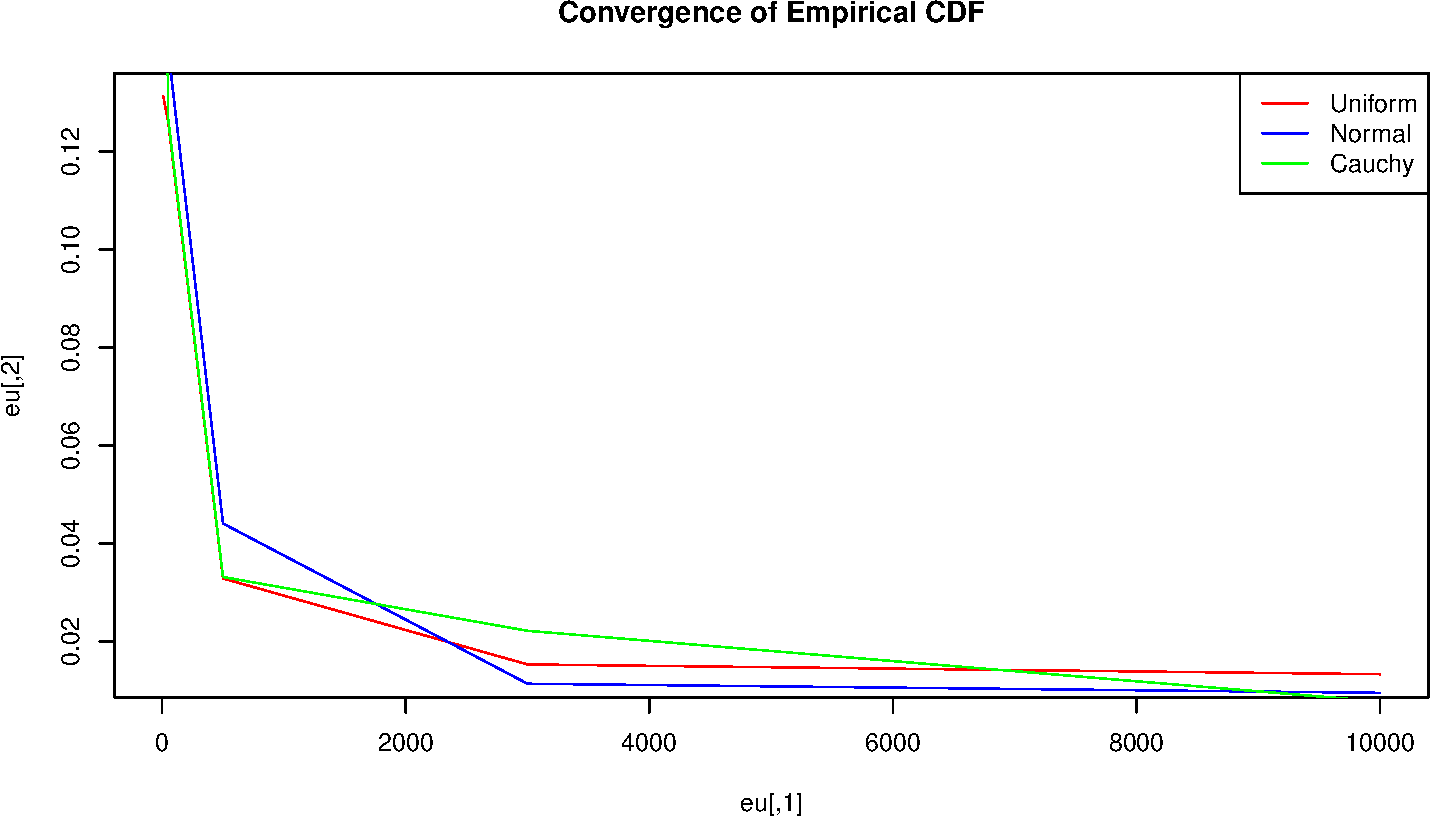
\includegraphics[width=0.7\linewidth,height=\textheight,keepaspectratio]{lln_files/figure-pdf/unnamed-chunk-1-1.pdf}

}

\caption{Figure: Illustration of Glivenko--Cantelli.}

\end{figure}%

\chapter{Central Limit Theorem}\label{sec-clt}

Gut (2014) 의 설명: i.i.d. rvs with mean \(\mu\)인
\(X, X_1, X_2,\ldots\)가 있을 때

\begin{itemize}
\item
  LLN:
  \(\frac{1}{n}\sum_{k=1}^n X_k \stackrel{n\rightarrow\infty}{\longrightarrow} \mu\)
  in prob or almost surely
\item
  CLT: \(\frac{1}{n}\sum_{k=1}-\mu\)를 ``blow up'' (아마 적절한 값을
  곱하고 나눈다는 뜻인듯)하여 \(n\rightarrow \infty\)일 때 어떤
  nontrivial한 분포에 수렴하는지 알려줌
\item
  물론, 흔히 아는 CLT는 variance가 존재할 때 앞선 통계량에
  \(\sqrt{n}\)을 곱하면 그 극한분포가 정규분포임을 의미
\item
  분산이 존재하지 않거나 summand가 독립이 아닌 상황에서의 CLT 등은
  Chapter~\ref{sec-limext} 참조
\end{itemize}

\section{The i.i.d. case}\label{the-i.i.d.-case}

\begin{theorem}[i.i.d., 유한분산일때의
CLT]\protect\hypertarget{thm-clt}{}\label{thm-clt}

Let \(X, X_1, X_2, \ldots\) be i.i.d. random variables with finite
expectation \(\mu\), and positive, finite variance \(\sigma^2\), and set
\(S_n = X_1 + X_2 + \cdots + X_n, n\geq 1\). Then \[
\frac{S_n - n\mu}{\sigma \sqrt{n}} \stackrel{d}{\rightarrow}\mathcal{N}(0,1), \quad{} \text{as }n \rightarrow\infty.
\]

\end{theorem}

\begin{tcolorbox}[enhanced jigsaw, left=2mm, arc=.35mm, leftrule=.75mm, colback=white, title=\textcolor{quarto-callout-note-color}{\faInfo}\hspace{0.5em}{Proof}, rightrule=.15mm, breakable, bottomrule=.15mm, coltitle=black, opacitybacktitle=0.6, opacityback=0, toptitle=1mm, titlerule=0mm, toprule=.15mm, colbacktitle=quarto-callout-note-color!10!white, bottomtitle=1mm, colframe=quarto-callout-note-color-frame]

특성함수에 대한 continuity theorem Theorem~\ref{thm-cfdistn} 의 관점에서
\[
\varphi_{\frac{S_n - n\mu}{\sigma \sqrt{n}}} (t) \rightarrow \infty e^{-t^2/2} \quad{} \text{as }n \rightarrow\infty, \text{ for} \quad{} -\infty < t < \infty
\] 일을 보이면 충분하다. 간단하게 \(\mu=0, \sigma=1\)이라고 두자. 그러면
특성함수의 성질에 의해 \[
\begin{align*}
\varphi_{\frac{S_n - n\mu}{\sigma \sqrt{n}}} (t) &=\varphi_{\frac{S_n }{\sqrt{n}}} (t) = \varphi_{S_n}\Big( \frac{t}{\sqrt{n}} \Big) = \Big( \varphi_X \Big( \frac{t}{\sqrt{n}}\Big)\Big)^n = \Big( 1- \frac{t^2}{2n} + o\Big( \frac{t^2}{n}\Big) \Big)^n\\
&\rightarrow e^{-t^2/2} \quad{} \text{as }n \rightarrow\infty.
\end{align*}
\]

\end{tcolorbox}

\section{The Lindeberg--Levy--Feller
Theorem}\label{the-lindeberglevyfeller-theorem}

\begin{itemize}
\item
  이번엔 summand가 independent이나 identically distributed는 아닌 상황을
  생각
\item
  이를 \(X_1, X_2, \ldots\) be independent random variable with finite
  variances, and set, for \(k\geq 1\), \(E(X_k) = \mu_k\)
  \(\text{var}(X_k) = \sigma_k^2\), and, for \(n\geq 1\),
  \(S_n =\sum_{k=1}^n X_k\), and \(s_n^2 = \sum_{k=1}^n \sigma_k^2\).
  그리고 degenerate한 케이스는 고려하지 않기로 한다.
\end{itemize}

\begin{definition}[Lindeberg
conditions]\protect\hypertarget{def-lindebergcond}{}\label{def-lindebergcond}

다음 두 개의 조건은 \textbf{Lindeberg conditions}라고 하며 general
form의 CLT와 관련이 있다. \[
\begin{align*}
L_1 (n) &= \max_{1\leq k \leq n} \frac{\sigma_k^2}{s_n^2} \rightarrow 0 \quad{} \text{as } n\rightarrow \infty,\\
L_2 (n) &= \frac{1}{s_n^2} \sum_{k=1}^n E(X_k - \mu_k)^2 I\{ |X_k - \mu_k | > \varepsilon s_n\} \stackrel{n\rightarrow \infty}{\longrightarrow}0.
\end{align*}
\]

\end{definition}

\begin{theorem}[Lindeberg--Levy--Feller
CLT]\protect\hypertarget{thm-lindebergclt}{}\label{thm-lindebergclt}

\(X_1, X_2,\ldots\)가 앞서와 같이 주어져 있다고 하자.

\begin{enumerate}
\def\labelenumi{\arabic{enumi}.}
\item
  만약 Definition~\ref{def-lindebergcond} 의 두 번째 식이 만족된다면,
  Definition~\ref{def-lindebergcond} 의 첫 번째 식도 만족되고 \[
  \frac{1}{s_n}\sum_{k=1}^n (X_k - \mu_k) \stackrel{d}{\rightarrow}\mathcal{N}(0,1) \quad{} \text{as }n\rightarrow\infty
  \] 도\textbf{(Lindeberg--Levy--Feller 버전의 CLT)} 만족한다.
\item
  만약 Definition~\ref{def-lindebergcond} 의 첫 번째 식과
  Lindeberg--Levy--Feller 버전의 CLT를 만족한다면,
  Definition~\ref{def-lindebergcond} 의 두 번째 식도 만족한다.
\end{enumerate}

\end{theorem}

\subsection{Lyapounov's Condition}\label{lyapounovs-condition}

\begin{itemize}
\tightlist
\item
  Lindeberg condition은 증명하기 어려운 측면이 있어 이것보다 약간 강한
  충분조건을 생각할 수 있는데 이것을 \textbf{Lyapounov condition}이라 함
\end{itemize}

\begin{theorem}[Lyapounov
condition]\protect\hypertarget{thm-lyapounovcond}{}\label{thm-lyapounovcond}

\(X_1, X_2,\ldots\)가 앞서와 같이 주어져 있다고 하자. 추가로
\(E\vert X_k \vert^r <\infty\) for all \(k\) and some \(r>2\)라고 하자.
만약 \[
\beta(n,r) = \frac{\sum_{k=1}^n E\vert |X_k - \mu_k \vert^r}{s_n^r} \rightarrow 0 \quad{} \text{as }n \rightarrow \infty
\] 를 만족한다면 Theorem~\ref{thm-lindebergclt} 의 CLT도 성립한다.

\end{theorem}

\chapter{The Law of the Iterated
Logarithm}\label{the-law-of-the-iterated-logarithm}

\section{The Law of the iterated logarithm
(LIL)}\label{the-law-of-the-iterated-logarithm-lil}

\begin{theorem}[Hartman and Wintner
LIL]\protect\hypertarget{thm-lil}{}\label{thm-lil}

~

\begin{itemize}
\item
  \(X, X_1, X_2, \ldots\)가 mean 0, variance \(\sigma^2 <0\)을 갖는
  i.i.d. 확률변수들이라고 하고 \(S_n = \sum_{k=1}^n X_k, n\geq 1\)이라고
  하면 \begin{equation}\phantomsection\label{eq-lil}{
  \lim\sup_{n\rightarrow\infty} (\lim\inf_{n\rightarrow\infty}) \frac{S_n}{\sqrt{2\sigma^2 n \log \log n}} = +1 (-1) \quad{} \text{a.s.}
  }\end{equation}
\item
  이를 간단히 쓰면 \[
  \lim\sup_{n\rightarrow\infty} \frac{|S_n|}{\sqrt{2\sigma^2 n \log \log n}} = 1 \quad{} \text{a.s.}
  \]
\item
  역으로 만약 \[
  P\Big( \lim\sup_{n\rightarrow\infty} \frac{|S_n|}{\sqrt{n \log \log n}} < \infty \Big) >0
  \] 이면 \(E(X^2)<\infty\), \(E(X)=0\), (Equation~\ref{eq-lil}) 이 성립
\end{itemize}

\end{theorem}

\begin{tcolorbox}[enhanced jigsaw, left=2mm, arc=.35mm, leftrule=.75mm, colback=white, title=\textcolor{quarto-callout-tip-color}{\faLightbulb}\hspace{0.5em}{Remark}, rightrule=.15mm, breakable, bottomrule=.15mm, coltitle=black, opacitybacktitle=0.6, opacityback=0, toptitle=1mm, titlerule=0mm, toprule=.15mm, colbacktitle=quarto-callout-tip-color!10!white, bottomtitle=1mm, colframe=quarto-callout-tip-color-frame]

왜 하필 \(\log \log n\)이라는 생각이 들 수도 있는데, 어떤 사람들은
normal distribution의 density에 \(\exp (-x^2/2)\)가 있어서 이 효과를
상쇄하려면 대략 \(\sqrt{\log \log n}\)을 쓰는 것으로 이해해 볼 수도 있음

\end{tcolorbox}

한편, Theorem~\ref{thm-lil} 과 같은 상황에서 체비세프 부등식을 적용하면
\[
P\Big( \Big\vert \frac{S_n}{\sqrt{2\sigma^2 n \log \log n}}  \Big\vert > \varepsilon \Big)\leq \frac{1}{2\varepsilon^2 \log \log n} \stackrel{n\rightarrow \infty}{\rightarrow} 0
\] 이기 때문에 \[
\frac{S_n}{\sqrt{2\sigma^2 n \log \log n}} \stackrel{p}{\rightarrow} 0 \quad{} \text{as }n \rightarrow \infty
\] 즉, \(\frac{S_n}{\sqrt{2\sigma^2 n \log \log n}}\)는 0으로
확률수렴한다.

그러나 sample-wise, path-wise (a.s. 관점에서)로는 \(-1\)과 \(1\)
사이에서 진동한다.

\section{R 코드}\label{r-uxcf54uxb4dc}

Haigh (2013) 의 Example 6.21

\textbf{Q}. Long-run behaviour of sums

\textbf{Q}. \(n\)이 증가함에 따라 \(S_n /\sqrt{n}\)의 fluctuations의
size는?

\subsection{Simulation setting}\label{simulation-setting}

\begin{itemize}
\item
  \(Y_n \stackrel{\text{indep}}{\sim} U(0,1)\)
\item
  \(X_n = Y_n \sqrt{12} - \sqrt{3}\), so that
  \(X_n \stackrel{\text{i.i.d.}}{\sim} U(-\sqrt{3}, \sqrt{3})\): 이렇게
  하면 \(E(X_n)=0, \text{Var}(X_n)=1\)이 됨
\item
  \(S_n = X_1 + \cdots X_n\)
\end{itemize}

\begin{figure}[H]

{\centering 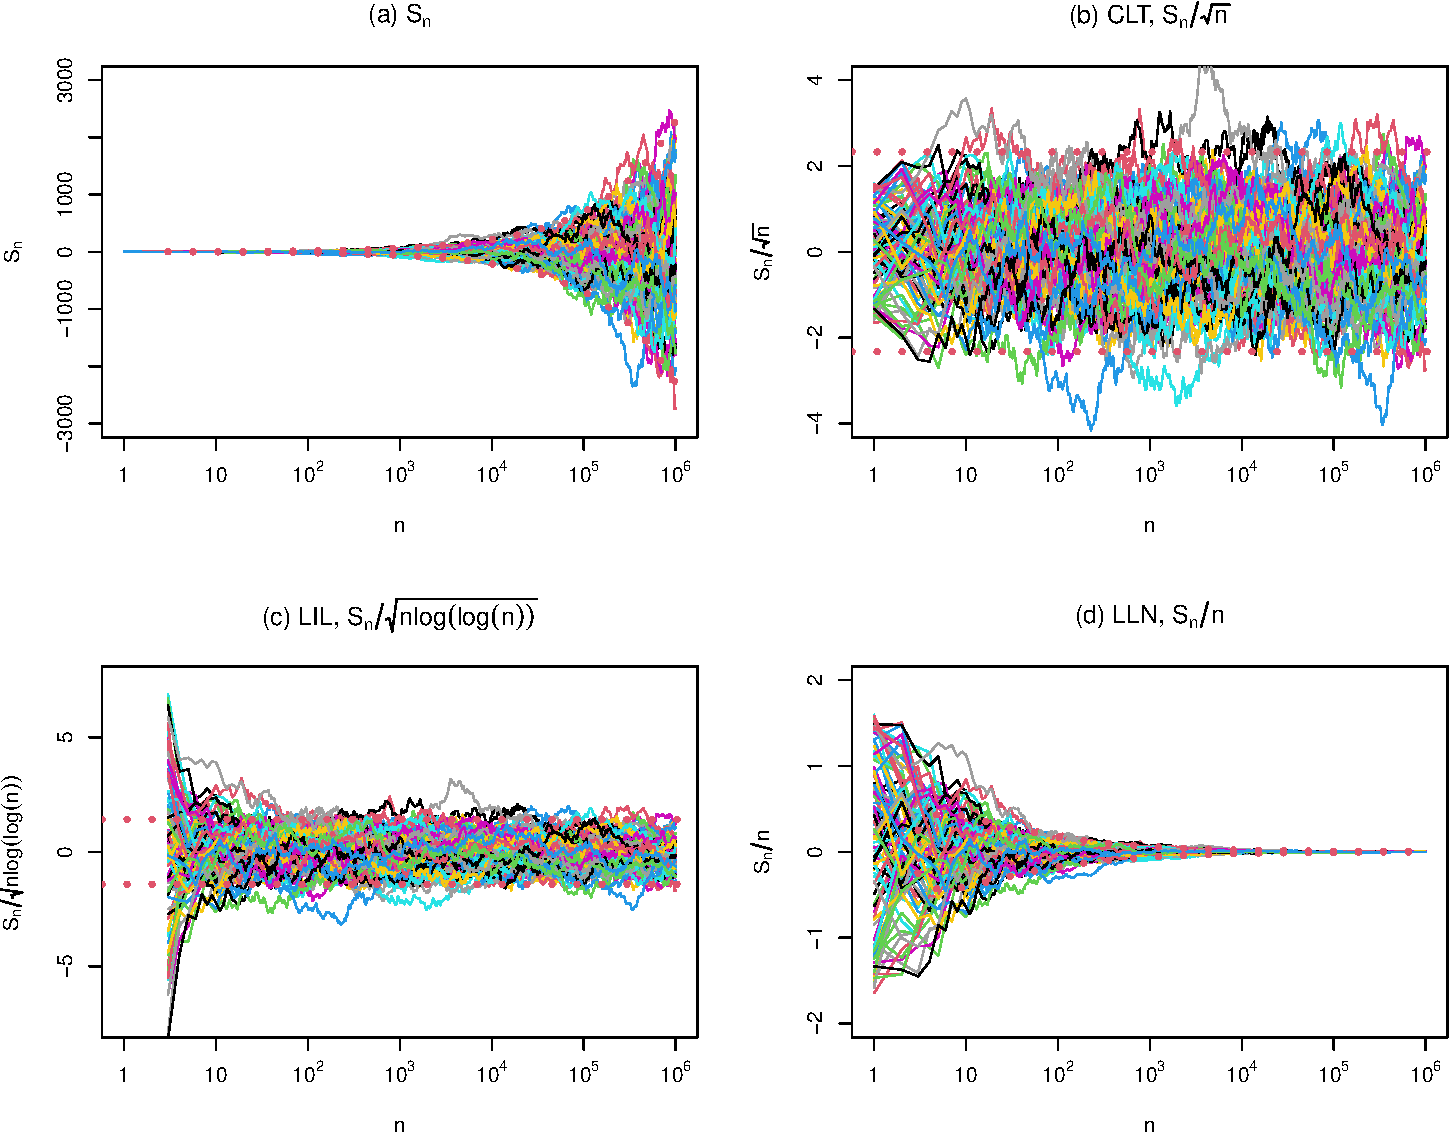
\includegraphics[width=0.7\linewidth,height=\textheight,keepaspectratio]{lil_files/figure-pdf/unnamed-chunk-2-1.pdf}

}

\caption{Figure: (a) Random sums. (b) CLT. (c) LIL. (d) LLN.}

\end{figure}%

\subsection{Results}\label{results}

\begin{itemize}
\item
  그림에 대한 추가 설명(참고로 모든 그림의 \texttt{x}축은
  \texttt{log}-스케일이다):

  \begin{itemize}
  \tightlist
  \item
    \begin{enumerate}
    \def\labelenumi{(\alph{enumi})}
    \tightlist
    \item
      \(n\)이 커짐에 따라 random sums \(S_n\)이 어떻게 되는지 보여줌,
      점선은 \(\pm \sqrt{2 n \log \log n}\)
    \end{enumerate}
  \item
    \begin{enumerate}
    \def\labelenumi{(\alph{enumi})}
    \setcounter{enumi}{1}
    \tightlist
    \item
      (CLT) \(n\)이 커짐에 따라 \(S_n/\sqrt{n}\)은 standard Gaussian으로
      분포수렴, 점선은 \(\pm \mathcal{N}^{-1}(0.01)\) (분위수)
    \end{enumerate}
  \item
    \begin{enumerate}
    \def\labelenumi{(\alph{enumi})}
    \setcounter{enumi}{2}
    \tightlist
    \item
      (LIL) \(n\)이 커짐에 따라 \(S_n/\sqrt{n\log \log n}\)은
      \([-\sqrt{2}, \sqrt{2}]\) 사이에 존재, 점선은 \(\pm \sqrt{2}\)
    \end{enumerate}
  \item
    \begin{enumerate}
    \def\labelenumi{(\alph{enumi})}
    \setcounter{enumi}{3}
    \tightlist
    \item
      (SLLN) \(n\)이 커짐에 따라 \(S_n/n \rightarrow 0\), 점선은
      \(\pm \sqrt{ \frac{2 \log \log n}{n}}\)
    \end{enumerate}
  \end{itemize}
\item
  SLLN: \(S_n / n \stackrel{n\rightarrow \infty}{\rightarrow} 0\) 임을
  말하는데, 이는 어떤 \(\varepsilon>0\)이 주어졌을 때,
  \(\forall n \geq N\)에 대해 \(S_n/n\)이 구간
  \((-\varepsilon, \varepsilon)\) 안에 있도록 하는 \(N\)이 존재
\item
  CLT: \(S_n /\sqrt{n} \stackrel{d}{\rightarrow} \mathcal{N}(0,1)\) 임을
  말하는데, 이는 \(n\)이 클때 \(P(-1< S_n /\sqrt{n} < 1) \approx 0.68\),
  \(P(|S_n /\sqrt{n}|>2)\approx 0.05\)임 등을 추론할 수 있음을 의미함

  \begin{itemize}
  \tightlist
  \item
    그러나 CLT가 boundedness를 말하는 것은 아니기 때문에 \(n\)이 매울 클
    때에도 매우 크거나 작은 \(S_n/\sqrt{n}\)이 나올 수 있음
  \end{itemize}
\item
  LIL: \(U_n = S_n / \sqrt{n \log (\log (n))}\)에 대해 말하는데,
  \(\sqrt{\log (\log (n))}\)은 unbounded지만 매우 \textbf{천천히}
  증가하는 함수임, \(n=10^6\)일 때 비로소
  \(\sqrt{\log (\log (n))}\approx 1.62\)가 됨

  \begin{itemize}
  \tightlist
  \item
    \(S_n\) 또한 \(n\)이 커질수록 천천히 변하기 때문에 \(U_n\)은 매우
    천천히 변할 것이라 생각할 수 있음
  \item
    그러나, \(\sqrt{\log (\log (n))}\)은 \(\mathcal{N}(0,1)\)의 변화를
    잡아줄 수 있을 정도로 큰 값이기는 함
  \end{itemize}
\item
  정리해보자면, LIL은 언젠가는 \(U_n\)이 \((-\sqrt{2},\sqrt{2})\)에 있을
  것임을 의미함
\end{itemize}

\chapter{Limit Theorems: Extensions and
Generalizations}\label{sec-limext}

\begin{itemize}
\item
  CLT나 LIL에서는 i.i.d. 확률변수의 sum에 대해 다룸
\item
  이때 유한한 분산을 추가로 가정함
\end{itemize}

\textbf{Q}. 만약 분산이 존재하지 않는다면?

\textbf{Q}. Summands가 더이상 독립이 아니라면?

\textbf{Q}. Sum으로부터 만들 수 있는 흥미있는 object들이 있는가?

\section{Stable distributions}\label{stable-distributions}

\begin{itemize}
\tightlist
\item
  Stable distribution의 정의에는 몇 가지가 있는 듯 (Nolan 2020)
\end{itemize}

\begin{definition}[Stable
distributions]\protect\hypertarget{def-stabledistn}{}\label{def-stabledistn}

~

\begin{itemize}
\item
  \(X_1, X_2, \ldots\)가 확률변수 \(X\)의 i.i.d. copy라 하고
  \(S_n, n\geq 1\)을 partial sum이라 하자. 만약 어떤 상수
  \(c_n > 0, d_n \in \mathbb{R}, n\geq 1\)이 존재해 \[
  S_n \stackrel{d}{=}c_n X + d_n, \quad{} \forall n
  \] 이라 하면 확률변수 \(X\)의 분포를 \textbf{stable in the broad
  sense}라고 함
\item
  만약 \(\forall n\)에 대해 \(d_n = 0\)이라고 하면 분포를
  \textbf{strictly stable}이라고 함
\end{itemize}

\end{definition}

\begin{tcolorbox}[enhanced jigsaw, left=2mm, arc=.35mm, leftrule=.75mm, colback=white, title=\textcolor{quarto-callout-tip-color}{\faLightbulb}\hspace{0.5em}{Remark}, rightrule=.15mm, breakable, bottomrule=.15mm, coltitle=black, opacitybacktitle=0.6, opacityback=0, toptitle=1mm, titlerule=0mm, toprule=.15mm, colbacktitle=quarto-callout-tip-color!10!white, bottomtitle=1mm, colframe=quarto-callout-tip-color-frame]

(Nolan (2020) 의 내용)

\begin{itemize}
\item
  Stable distribution은 skeness, heavy-tail 등을 다룰 수 있는
  probability distn의 큰 클래스이며 좋은 수학적 성질도 가지고 있다고 함
\item
  문제점: Gaussian, Cauchy, Levy 등을 제외하면 density와 distn에 대한
  closed formula가 부족하다는 단점 존재
\item
  그러나 컴퓨터 프로그램의 도움을 받아 stable distn의 density나 distn
  등을 계산할 수 있음
\end{itemize}

\end{tcolorbox}

\part{Stochastic Processes}

\part{Extremes}

\chapter{Heavy-Tailed Distributions}\label{heavy-tailed-distributions}

\section{Heavy-tailed distributions}\label{heavy-tailed-distributions-1}

\begin{definition}[]\protect\hypertarget{def-taifct}{}\label{def-taifct}

~

\begin{itemize}
\item
  \textbf{Tail function} \(\overline{F}\) of a distribution \(F\) on
  \(\mathbb{R}\) to be given by
  \(\overline{F}(x) = F(x,\infty), \forall x\).
\item
  \textbf{Tail property} of \(F\): any property which depends only on
  \(\{ \overline{F} (x) : x \geq x_0 \}\) for any (finite) \(x_0\).
\item
  We say that \(F\) has \textbf{right-unbounded support} if
  \(\overline{F}(x) >0, \forall x\).
\end{itemize}

\end{definition}

\begin{definition}[Heavy-tailed
distributions]\protect\hypertarget{def-heavytaileddist}{}\label{def-heavytaileddist}

~

\begin{itemize}
\item
  A distribution \(F\) on \(\mathbb{R}\) is said to be \textbf{right
  heavy-tailed} if \[
  \int_{-\infty}^{\infty}e^{\lambda x} F(dx) = \infty, \quad{} \forall \lambda >0,
  \] that is, iff \(F\) fails to posses any positive exponential moment.
\item
  Otherwise \(F\) is said to be \textbf{light-tailed}.
\end{itemize}

\end{definition}

\begin{definition}[Long-tailed
distributions]\protect\hypertarget{def-longtaileddist}{}\label{def-longtaileddist}

~

\begin{itemize}
\tightlist
\item
  A distribution \(F\) on \(\mathbb{R}\) is said to be
  \textbf{long-tailed} if \(F\) has right-unbounded support and, for any
  fixed \(y>0\), \[
  \frac{\overline{F}(x+y)}{\overline{F}(x)} \rightarrow 1, \quad{} \text{as } x \rightarrow \infty.
  \]
\end{itemize}

\end{definition}

\begin{tcolorbox}[enhanced jigsaw, left=2mm, arc=.35mm, leftrule=.75mm, colback=white, title=\textcolor{quarto-callout-tip-color}{\faLightbulb}\hspace{0.5em}{Remark}, rightrule=.15mm, breakable, bottomrule=.15mm, coltitle=black, opacitybacktitle=0.6, opacityback=0, toptitle=1mm, titlerule=0mm, toprule=.15mm, colbacktitle=quarto-callout-tip-color!10!white, bottomtitle=1mm, colframe=quarto-callout-tip-color-frame]

\begin{itemize}
\item
  Clearly to be long-tailed is again a tail property of a distribution.
\item
  Further, it is fairly easy to see that a long-tailed distribution is
  also heavy-tailed.
\end{itemize}

\end{tcolorbox}

\begin{definition}[Subexponential
distributions]\protect\hypertarget{def-longtaileddist}{}\label{def-longtaileddist}

~

\begin{itemize}
\tightlist
\item
  A distribution \(F\) on \(\mathbb{R}^{+}\) is said to be
  \textbf{subexponential} if \[
  \lim_{x\rightarrow\infty}\frac{\overline{F * F}(x)}{\overline{F}(x)}=2.
  \]
\end{itemize}

\end{definition}

\section{Examples of heavy-tailed
distributions}\label{examples-of-heavy-tailed-distributions}

\chapter{Multivariate Extreme Value
Theory}\label{multivariate-extreme-value-theory}

\section{Pseudo-Polar Transforms}\label{pseudo-polar-transforms}

Kiriliouk et al.~(2016) describe a \textbf{pseudo-polar} representation
of bivariate data as a means to explore right-tail extremal dependency
between the variables.

Let \((X_i, Y_i)\) (real values) or \((U_i, V_i)\) (as probabilities)
for \(i=1,\ldots, n\) be a bivariate sample of size \(n\). When such
data are transformed into a \textbf{unit-Pareto} scale by \[
\hat{X}_i^{*} = \frac{n}{n+1-R_{X,i}}, \quad{} \hat{Y}_i^{*} = \frac{n}{n+1-R_{Y,i}},
\] where \(R\) is \texttt{rank()}, then letting each \textbf{component
sum} or \textbf{pseudo-polar radius} be defined as \[
\hat{S}_i = \hat{X}_i^{*} + \hat{Y}_i^{*},
\] and each respective \textbf{pseudo-polar angle} be defined as \[
\hat{W}_i = \frac{\hat{X}_i^{*}}{\hat{X}_i^{*} + \hat{Y}_i^{*}} = \frac{\hat{X}_i^{*}}{\hat{S}_i}
\] a \textbf{pseudo-polar representation} is available for study.

A scatter plot of \(\hat{W}_i\) (horizontal) versus \(\hat{S}_i\)
(vertical) will depict a \textbf{pseudo-polar plot} of the data.

A density plot of the \(\hat{W}_i\) is a representation of extremal
dependence.

\begin{figure}[H]

{\centering 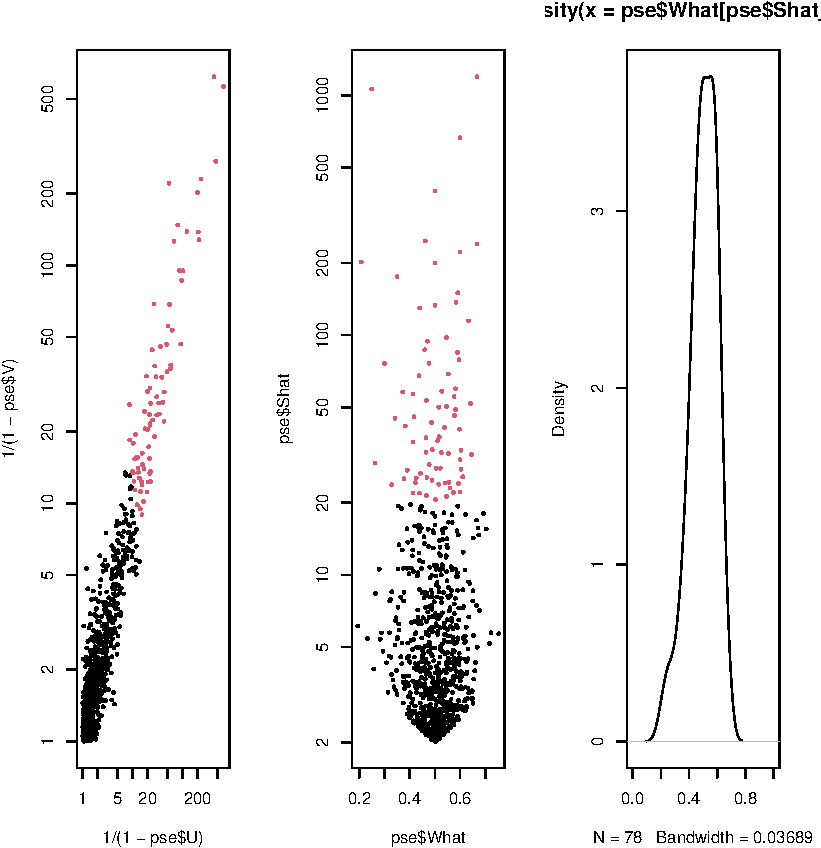
\includegraphics[width=0.7\linewidth,height=\textheight,keepaspectratio]{mev_files/figure-pdf/unnamed-chunk-1-1.pdf}

}

\caption{Figure: Extremal dependence.}

\end{figure}%

\section{Clustering Methods in
Extremes}\label{clustering-methods-in-extremes}

\begin{itemize}
\item
  Handbook on Statistics of Extremes 책 발간 예정
\item
  Vector quantization
\end{itemize}

\subsection{K-means clustering}\label{k-means-clustering}

\begin{itemize}
\item
  Given obs \(\pmb{x}_1, \ldots, \pmb{x}_n\), find \(K\) cluster
  centroids \(\pmb{c}_1, \ldots, \pmb{c}_K\) s.t. the avg
  data-point-to-centroid dist is minimized: \[
  (\pmb{c}_1, \ldots, \pmb{c}_K) := \arg\min_{\pmb{c}_1, \ldots, \pmb{c}_K} \sum_{k=1}^K 
  \]
\item
  Estimate the centroids \(\pmb{c}_k\) and the cluster membership of
  each \(\pmb{x}_i\) in turns.

  \begin{itemize}
  \tightlist
  \item
    Given \(\hat{\pmb{c}}_1, \ldots, \hat{\pmb{c}}_K\), assign
    \(\pmb{x}_i\) to the cluster \(k\) with the closest centroid
    \(\hat{\pmb{c}}_k\). \[
    i \in C_k \Longleftrightarrow d(\pmb{x}_i, c_k) = \min_{k'}d(\pmb{x}_i, \pmb{c}_{k'})
    \]
  \item
    Given all \(\pmb{x}_i\)'s in cluster \(k\), update each
    \(\hat{\pmb{c}}_k\)
  \end{itemize}
\end{itemize}

\textbf{Q}. Choice of \(d(\cdot, \cdot)\): + Euclidean
\(d(\pmb{x}, \pmb{y}) = (\pmb{x}- \pmb{y})^T(\pmb{x}- \pmb{y})\) + Then
the centroids can be calculated as \[
  \hat{\pmb{c}}_k = \arg\min_{\pmb{c}} \sum_{i\in C_k}(\pmb{x}_i - \pmb{c})^T(\pmb{x}_i - \pmb{c}) = \frac{1}{|C_k|} \sum_{i\in C_k}
  \]

\textbf{Q}. Choice of \(K\): + Prespecified + Use a scree plot where the
obj fct \[
  \min_{\pmb{c}_1, \ldots, \pmb{c}_K} \sum_{k=1}^K \sum_{i \in C_k} d(\pmb{x}_i , \pmb{c}_k)
  \]

이러한 \(K\)-mean 같이 Euclidean dist를 쓰는 방법은 extreme value에서
통하기 어려움

\section{Spectral Clustering}\label{spectral-clustering}

\begin{itemize}
\item
  Can detect nonlinear cluster patterns
\item
  Can identify noise clusters
\end{itemize}

\section{Clustering the Angluar
Components}\label{clustering-the-angluar-components}

\begin{itemize}
\item
  \(\pmb{Y}\) be multivariate regularly varying with standardized margin
  (Frechet 등이 해당) Then \[
  \frac{\pmb{Y}}{\|\pmb{Y}\|}_{\| \pmb{Y}\|>t}\stackrel{d}{\rightarrow} \Theta, \quad{} t \rightarrow \infty.
  \]
\item
  Clustering for extremes:

  \begin{itemize}
  \tightlist
  \item
    Obtain angular compts \(\Theta_1, \ldots, \Theta_{k_n}\) from
    \(\pmb{Y}_1, \ldots , \pmb{Y}_n\)
  \item
    Cluster \(\Theta_1, \ldots, \Theta_{k_n}\) instead.
  \end{itemize}
\end{itemize}

여기서 \(\Theta\)는 unit sphere \(\{ \pmb{x} \| \pmb{x} \| = 1\}\)이라는
매우 좋은 space에 놓여 있다. (이때 \(\| \cdot \|\)은 any norm이나 되지만
\(L2\) norm을 쓰기로 한다)

\section{Max-Linear Models}\label{max-linear-models}

\begin{itemize}
\item
  Max-linear random vector: \[
  \pmb{X} = (X_1, \ldots, X_d) = \vee_{i=1, \ldots, K}\pmb{b}_i Z_i
  \]
\item
  Factors \(\pmb{b}_1, \ldots, \pmb{b}_{K} \in [ 0, \infty )^{d}\)
\item
  \(Z_1, \ldots, Z_k\): i.i.d. Frechet
\end{itemize}

Then the angular measure \(\Theta\) consists of point masses at \[
\frac{\pmb{b}_1}{\|\pmb{b}_1\|}, \ldots
\]

\subsection{\texorpdfstring{Spherical
\(K\)-means}{Spherical K-means}}\label{spherical-k-means}

\begin{itemize}
\tightlist
\item
  Apply to \(\Theta_1, \ldots, \Theta_{k_n}\): \(K\)-means clustering
  with choice of distance \[
  d(\pmb{x}, \pmb{y}) = 1- \cos (\pmb{x}, \pmb{y})
  \]
\end{itemize}

On the unit sphere \(\mathbb{S}_{+}^{d-1}\),

\begin{itemize}
\tightlist
\item
  \(d(\pmb{x}, \pmb{y})= 1-\pmb{x}^T\pmb{y}\)
\item
  \(d\) is equiv to the Euclidean dist
\end{itemize}

\subsection{\texorpdfstring{Spherical \(K\)-PCs clustering for
extremes}{Spherical K-PCs clustering for extremes}}\label{spherical-k-pcs-clustering-for-extremes}

\begin{itemize}
\item
  앞선 방법과 달리 \(d(\pmb{x}, \pmb{y}) = 1-(\pmb{x}^T\pmb{y})^2\)을
  쓰는 것이 차이점(제곱이 들어감)
\item
  https://academic.oup.com/biomet/article-abstract/110/1/135/6551983?redirectedFrom=PDF
\item
  \(\arg\max_{\|\pmb{c}\|_2=1} \pmb{c}^T\Sigma_k \pmb{c}\) 형태가 나옴
\item
  For any spectral measure that can be decomposed into two sub-faces
  \(l_1\) and \(l_2\), we would like the optimal centroids to satisfy \[
  \pmb{c}_1 \in \mathbb{F}_{l_1}, \quad{} \pmb{c}_2 \in \mathbb{F}_{l_2}
  \]
\item
  This holds for spheical \(K\)-means iff \[
  \|l_1 | - | l_2 \| \leq 1
  \]
\item
  This holds for spherical \(K\)-PCs always.
\item
  If angular components \(\pmb{x}\) and \(\pmb{y}\) belongs to different
  sub-faces, then \(\pmb{x}^T\pmb{y}\) close to \(0\).
\end{itemize}

\subsection{Spectral clustering for
extremes}\label{spectral-clustering-for-extremes}

\begin{itemize}
\tightlist
\item
  Linear factor model with noise: \[
  \pmb{X} = (X_1, \ldots, X_d) = \sum_{i=1}^K
  \]
\end{itemize}

\part{High-Dimensional Probability}

\chapter{Random Matrices}\label{random-matrices}

\section{Intro: R 예제}\label{intro-r-uxc608uxc81c}

\subsection{실험 1: Normal random symmetric
matrix}\label{uxc2e4uxd5d8-1-normal-random-symmetric-matrix}

\begin{itemize}
\item
  \(A_{ij} \sim \mathcal{N}(0,1)\)에서 \(5000\times 5000\) random
  symmetric matrix 작성
\item
  Eigenvalue 계산 후 histogram 그림
\end{itemize}

\subsection{실험 2: Uniform random symmetric
matrix}\label{uxc2e4uxd5d8-2-uniform-random-symmetric-matrix}

\begin{itemize}
\item
  \(A_{ij} \sim \text{Uniform}(0,1)\)에서 \(5000\times 5000\) random
  symmetric matrix 작성
\item
  Eigenvalue 계산 후 histogram 그림
\end{itemize}

\begin{figure}[H]

{\centering 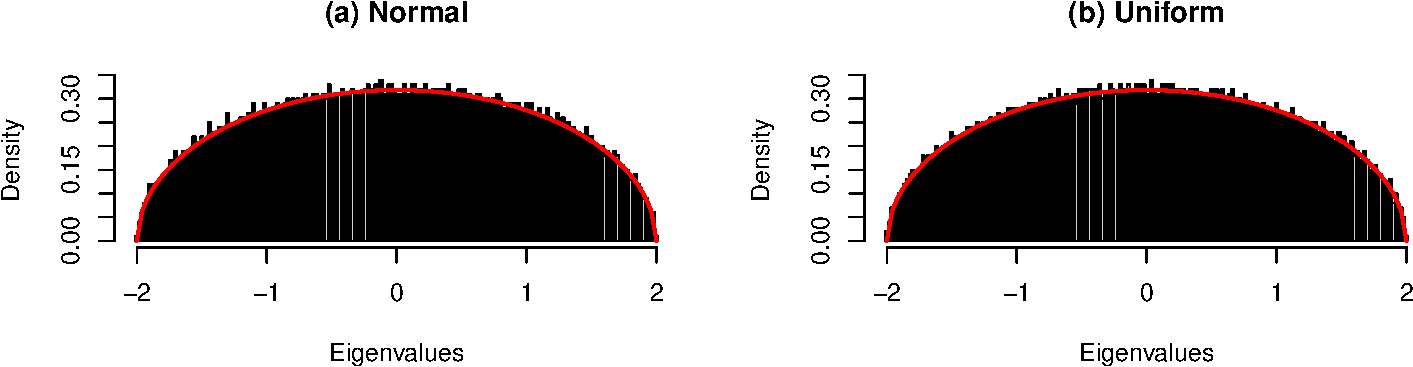
\includegraphics[width=0.7\linewidth,height=\textheight,keepaspectratio]{rmatrices_files/figure-pdf/unnamed-chunk-2-1.pdf}

}

\caption{Figure: (왼쪽) Normal random matrix의 eigenvalue의
distribution. (오른쪽) Uniform random matrix의 eigenvalue의
distribution.}

\end{figure}%

\begin{itemize}
\tightlist
\item
  붉은 선은
  \href{https://en.wikipedia.org/wiki/Wigner_semicircle_distribution}{Wigner
  semicircle distribution}
\end{itemize}

\part{Appendix}

\chapter{Order Notation}\label{order-notation}

출처:

\begin{itemize}
\tightlist
\item
  (García-Portugués 2024)
\end{itemize}

\section{\texorpdfstring{Big \(O\) and small \(o\) notation
(deterministic
versions)}{Big O and small o notation (deterministic versions)}}\label{big-o-and-small-o-notation-deterministic-versions}

\begin{itemize}
\tightlist
\item
  In mathematical analysis, \(O\)-related notation is mostly used to
  bound sequences that shrink to \(0\).
\end{itemize}

\begin{definition}[Big-\(O\)]\protect\hypertarget{def-bigoh}{}\label{def-bigoh}

Given two strictly positive sequence \(a_n\) and \(b_n\), \[
a_n = O(b_n): \Longleftrightarrow \text{limsup}_{n\rightarrow \infty}\frac{a_n}{b_n} \leq C, \quad{} \text{for a } C>0
\] If \(a_n = O(b_n)\), then we say that \(a_n\) is \textbf{big-O} of
\(b_n\). To indicate that \(a_n\) is bounded, we write \(a_n = O(1)\).

\end{definition}

For a deterministic sequence \(a_n\),
\(\text{limsup}_{n\rightarrow \infty}:=\lim_{n\rightarrow \infty}(\sup_{k \geq n} a_k)\)
is the largest limit of the subsequences of \(a_n\). It can be defined
even if \(\lim_{n\rightarrow\infty}a_n\) does not exist (e.g., in
trigonometric functions). If \(\lim_{n\rightarrow\infty} a_n\) exists,
as in most of the common usages of the big-\(O\) notation, then
\(\text{limsup}_{n\rightarrow\infty}a_n = \lim_{n\rightarrow\infty}a_n\).

\begin{definition}[Little-\(o\)]\protect\hypertarget{def-littleoh}{}\label{def-littleoh}

Given two strictly positive sequence \(a_n\) and \(b_n\), \[
a_n = o(b_n): \Longleftrightarrow \lim_{n\rightarrow\infty} \frac{a_n}{b_n} = 0.
\] If \(a_n = o(b_n)\), then we say that \(a_n\) is \textbf{little-o} of
\(b_n\). To indicate that \(a_n\rightarrow 0\), we write \(a_n = o(1)\).

\end{definition}

\begin{definition}[Asymptotically
equivalent]\protect\hypertarget{def-asymptequiv}{}\label{def-asymptequiv}

(Polansky 2011) The notation \(x_n \asymp y_n\) means that \[
\lim_{n\rightarrow\infty} \frac{x_n}{y_n}=1,
\] or that the two sequences are \textbf{asymptotically equivalent} as
\(n\rightarrow\infty\).

\end{definition}

\begin{tcolorbox}[enhanced jigsaw, left=2mm, arc=.35mm, leftrule=.75mm, colback=white, title=\textcolor{quarto-callout-tip-color}{\faLightbulb}\hspace{0.5em}{Remark}, rightrule=.15mm, breakable, bottomrule=.15mm, coltitle=black, opacitybacktitle=0.6, opacityback=0, toptitle=1mm, titlerule=0mm, toprule=.15mm, colbacktitle=quarto-callout-tip-color!10!white, bottomtitle=1mm, colframe=quarto-callout-tip-color-frame]

Order notation로 asymptotic behavior를 표현하는 것은 unique하지 않다.
(Polansky 2011) 예를 들어 \(a_n = O(n^{-1})\)이라고 하자. 그렇다는 것은
\(\vert n a_n \vert\)가 모든 \(n\in \mathbb{N}\)에 대해 bounded하다는
것이다. 그런데 \(|n^{1/2}a_n| \leq |na_n|\),
\(\forall n\in\mathbb{N}\)이므로, \(a_n = O(n^{-1/2})\)이기도 하다.

\end{tcolorbox}

\begin{exercise}[]\protect\hypertarget{exr-bigohlittleoh}{}\label{exr-bigohlittleoh}

~

\begin{enumerate}
\def\labelenumi{\arabic{enumi}.}
\tightlist
\item
  \(n^{-2} =o(n^{-1})\) since
  \(\lim_{n\rightarrow\infty}\frac{n^{-2}}{n^{-1}}\lim_{n\rightarrow\infty}\frac{1}{n}=0\)
\end{enumerate}

\begin{enumerate}
\def\labelenumi{\arabic{enumi}.}
\setcounter{enumi}{1}
\item
  \(\log n = O(n)\): We want to show that
  \(\forall n\geq 1, \log (n) \leq n\). The proof is by indunction on
  \(n\). The claim is true for \(n=1\), since \(0<1\). Now suppose
  \(n\geq 1\) and \(\log (n) \leq n\). Since \(n+1\leq 2n\), (밑이 2인
  로그를 쓴 듯) \[
  \log (n+1) \leq \log (2n) = \log(n) + 1 \leq n+1
  \] or \[
  \log (n+1) = \log n \log (1 + \frac{1}{n}) < n + \log (1 + \frac{1}{n}) < n+1 \because \text{ since } \log 2 < 1
  \]
\item
  \(n^{-1} = o((\log n)^{-1})\): 로피탈의 정리를 쓰면 \[
  \lim_{n\rightarrow \infty} \frac{n^{-1}}{(\log n)^{-1}}=\lim_{n\rightarrow \infty}  \frac{\log n}{n}=0
  \] 임을 보일 수 있음
\item
  \(n^{-4/5} = o(n^{-2/3})\) \[
  \lim_{n\rightarrow \infty} \frac{n^{-4/5}}{n^{-2/3}} = \lim_{n\rightarrow \infty} n^{2/3 - 4/5} = \lim_{n\rightarrow\infty} n^{-2/15}=0  
  \] 으로 알 수 있음
\item
  \(3\sin (n) = O(1)\): \(\sin\)함수는 진동함수이다.
\end{enumerate}

\end{exercise}

\begin{tcolorbox}[enhanced jigsaw, left=2mm, arc=.35mm, leftrule=.75mm, colback=white, title=\textcolor{quarto-callout-tip-color}{\faLightbulb}\hspace{0.5em}{Remark}, rightrule=.15mm, breakable, bottomrule=.15mm, coltitle=black, opacitybacktitle=0.6, opacityback=0, toptitle=1mm, titlerule=0mm, toprule=.15mm, colbacktitle=quarto-callout-tip-color!10!white, bottomtitle=1mm, colframe=quarto-callout-tip-color-frame]

Big-O, small-o의 정의로부터 다음을 알 수 있다.

\begin{itemize}
\item
  \(a_n = O(b_n)\) means that \(a_n\) is \textbf{not larger than}
  \(b_n\) asymptotically. If \(a_n , b_n \rightarrow 0\), then it means
  that \(a_n\) \textbf{does not decrease more slowly} than \(b_n\),
  i.e., that \(a_n\) either decreases as fast as \(b_n\) or faster than
  \(b_n\).
\item
  \(a_n = o(b_n)\) means that \(a_n\) is \textbf{smaller than} \(b_n\)
  asymptotically. If \(a_n, b_n \rightarrow 0\), then it means that
  \(a_n\) \textbf{decrease faster} than \(b_n\).
\end{itemize}

위의 사실로부터, big-O는 같은 속도로 수렴하거나 더 빠른 속도로 수렴하는
두 가지 경우를 모두 포함하고 있고, small-o는 더 빠른 속도로 수렴하는
경우만 포함하기 때문에 어떤 \(C>0\)에 대해 \textbf{little-o implies
big-O}라고 할 수 있다.

\end{tcolorbox}

다음은 (García-Portugués 2024)에 적혀 있는 big-O, small-o에 대한 몇 가지
성질들이다.

\begin{proposition}[]\protect\hypertarget{prp-bigolittleo}{}\label{prp-bigolittleo}

Consider two strictly positive sequences \(a_n, b_n \rightarrow 0\). The
following properties hold (García-Portugués 2024):

\begin{enumerate}
\def\labelenumi{\arabic{enumi}.}
\item
  \(kO(a_n) = O(a_n)\), \(ko(a_n) = o(a_n)\), \(k\mathbb{R}\).
\item
  \(o(a_n) + o(b_n) = o(a_n + b_n)\),
  \(O(a_n) + O(b_n) = O(a_n + b_n)\).
\item
  \(o(a_n)o(b_n) = o(a_nb_n)\), \(O(a_n)O(b_n) = O(a_nb_n)\).
\item
  \(o(a_n) + O(b_n) = O(a_n + b_n)\), \(o(a_n)O(b_n) = o(a_nb_n)\).
\item
  \(o(1)O(a_n) = o(a_n)\).
\item
  \(a_n^r = o(a_n^s)\), for \(r>s\geq 0\).
\item
  \(a_nb_n =o(a_n^2 +b_n^2)\) (아마 \(O(a_n^2 + b_n^2)\)이 되어야 할 듯)
\item
  \((a_n + b_n)^k = O(a_n^k + b_n^k)\).
\end{enumerate}

\end{proposition}

\begin{longtable}[]{@{}
  >{\raggedright\arraybackslash}p{(\linewidth - 2\tabcolsep) * \real{0.5833}}
  >{\raggedright\arraybackslash}p{(\linewidth - 2\tabcolsep) * \real{0.4167}}@{}}
\toprule\noalign{}
\begin{minipage}[b]{\linewidth}\raggedright
Sequence
\end{minipage} & \begin{minipage}[b]{\linewidth}\raggedright
Result
\end{minipage} \\
\midrule\noalign{}
\endhead
\bottomrule\noalign{}
\endlastfoot
\(b_n = 1/\log (n)\) & \\
\(a_{1,n}=\frac{2}{n}+\frac{50}{n^2}\) & \(o(b_n)\) (hence also
\(O(b_n)\)) \\
\(a_{2,n}=\frac{\sin (n/5)+2}{n^{5/4}}\) & \(o(b_n)\) (hence also
\(O(b_n)\)) \\
\(a_{3,n}=\frac{3(1+5\exp(-(n-55.5)^2/200))}{n}\) & \(o(b_n)\) (hence
also \(O(b_n)\)) \\
\(a_{4,n}=\frac{n+3}{4n\log_{10}(n)}+\frac{a_{3,n}}{2}\) & \(O(b_n)\),
but not \(o(b_n)\) \\
\(a_{5,n}=\frac{1}{4\log_{2} (\frac{n}{2})}\) & \(O(b_n)\), but not
\(o(b_n)\) \\
\(a_{6,n}=\frac{1}{\log (n^2+n)}\) & \(O(b_n)\), but not \(o(b_n)\) \\
\(a_{7,n}=\frac{1}{2\log(5n+3)^{1/4}}\) & not \(O(b_n)\) (hence neither
\(o(b_n)\)) \\
\(a_{8,n}=\frac{1}{4\log(\log (10n+2))}\) & not \(O(b_n)\) (hence
neither \(o(b_n)\)) \\
\(a_{9,n}=\frac{1}{2\log(\log (n^2+10n+2))}\) & not \(O(b_n)\) (hence
neither \(o(b_n)\)) \\
\end{longtable}

\begin{center}
\pandocbounded{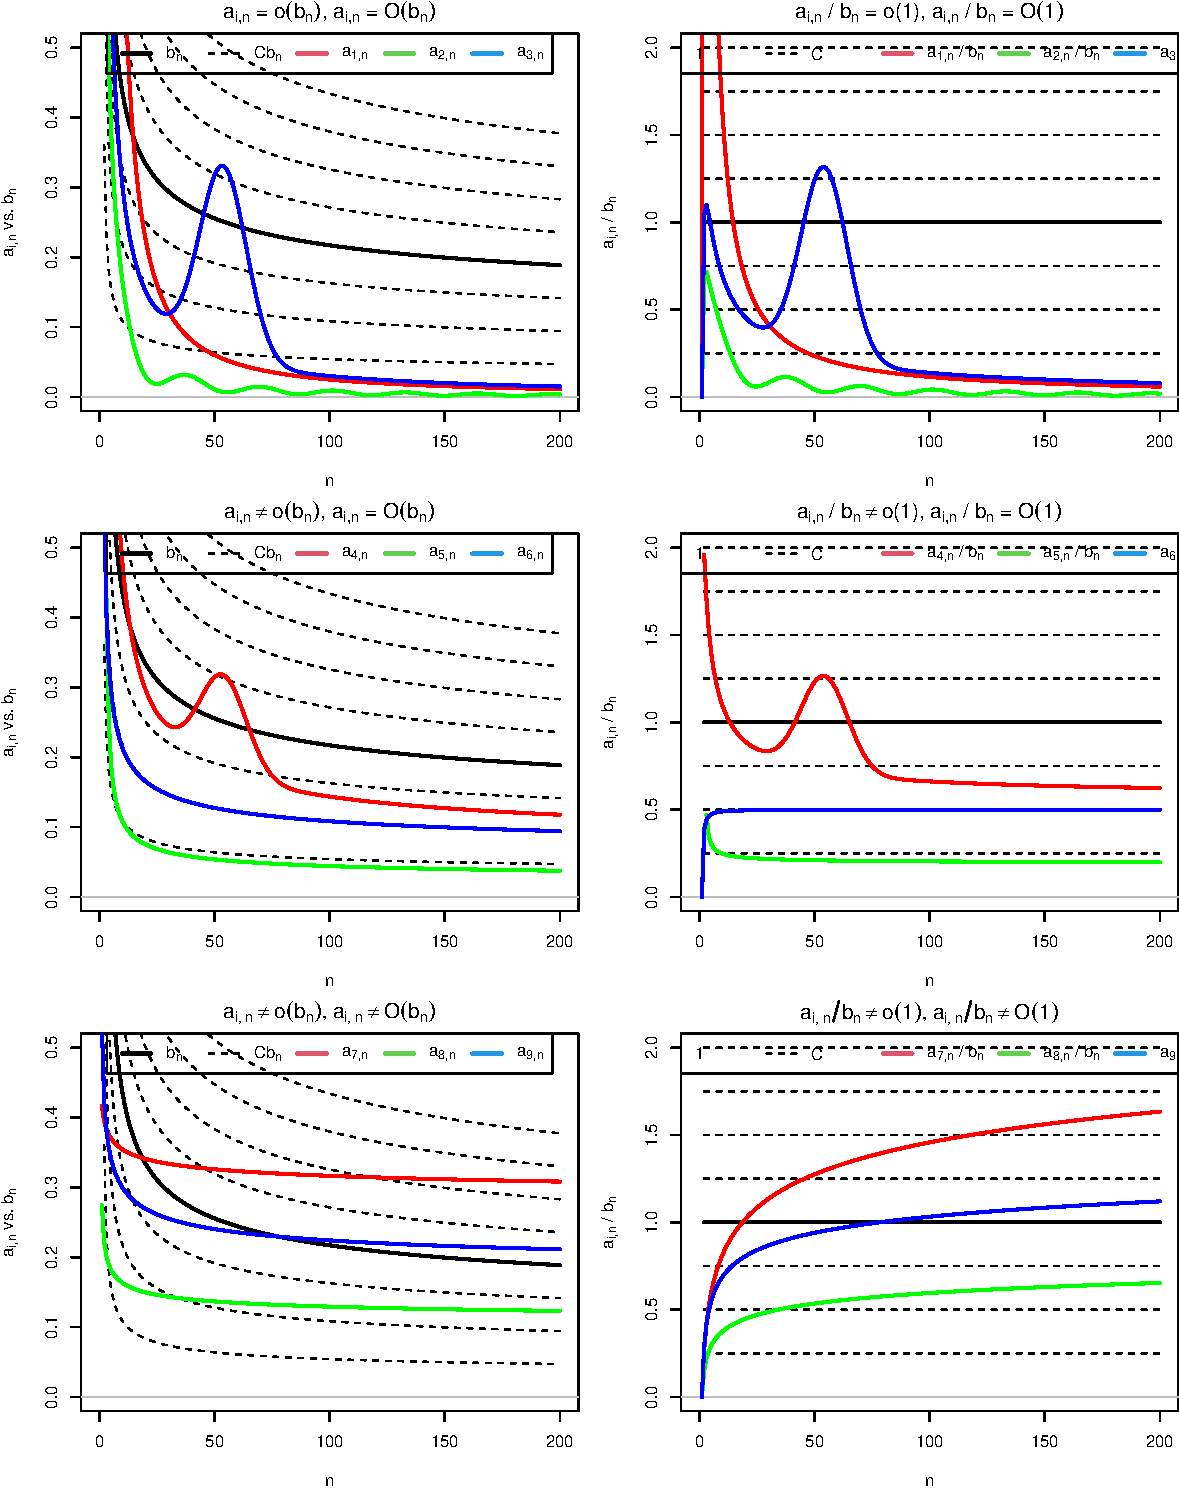
\includegraphics[keepaspectratio]{bigoh_files/figure-pdf/unnamed-chunk-1-1.pdf}}
\end{center}

\begin{tcolorbox}[enhanced jigsaw, left=2mm, arc=.35mm, leftrule=.75mm, colback=white, title=\textcolor{quarto-callout-tip-color}{\faLightbulb}\hspace{0.5em}{Remark}, rightrule=.15mm, breakable, bottomrule=.15mm, coltitle=black, opacitybacktitle=0.6, opacityback=0, toptitle=1mm, titlerule=0mm, toprule=.15mm, colbacktitle=quarto-callout-tip-color!10!white, bottomtitle=1mm, colframe=quarto-callout-tip-color-frame]

\begin{itemize}
\tightlist
\item
  오른쪽의 그림들을 보면 수렴에 대해 파악할 수 있음

  \begin{itemize}
  \tightlist
  \item
    위: \(\frac{a_{i,n}}{b_{n}}\)이 \(n\rightarrow \infty\)일 때 0으로
    수렴, 따라서 \(\frac{a_{i,n}}{b_{n}}=\mathcal{o}(1)\) 이고
    \(\frac{a_{i,n}}{b_{n}}=\mathcal{O}(1)\)임
  \item
    가운데: \(\frac{a_{i,n}}{b_{n}}\)이 \(n\rightarrow \infty\)일 때 0이
    아닌 어떤 값으로 수렴하는 것처럼 보임, 따라서
    \(\frac{a_{i,n}}{b_{n}}\neq\mathcal{o}(1)\) 이나
    \(\frac{a_{i,n}}{b_{n}}=\mathcal{O}(1)\)임
  \item
    아래: \(\frac{a_{i,n}}{b_{n}}\)이 \(n\rightarrow \infty\)일 때
    발산하는 것으로 보이며 따라서
    \(\frac{a_{i,n}}{b_{n}}\neq\mathcal{o}(1)\) 이고
    \(\frac{a_{i,n}}{b_{n}}\neq\mathcal{O}(1)\)임
  \end{itemize}
\end{itemize}

\end{tcolorbox}

다음은 (García-Portugués 2024)가 소개한 \(C_p\) inequality이다.

\begin{lemma}[\(C_p\)
inequality]\protect\hypertarget{lem-Cp}{}\label{lem-Cp}

Given \(a,b\in \mathbb{R}\) and \(p>0\), \[
|a+b|^p \leq C_p (|a|^p + |b|^p), \quad{} C_p=
\begin{cases}
1, & p\leq 1\\
2^{p-1}, & p >1.
\end{cases}
\]

\end{lemma}

다음으로 생각해 볼 만한 것은 \(n\rightarrow\infty\)일 때
\(O(n^{-1/2})\)와 \(O(n^{-1})\)처럼 차수가 다른 수열의 수렴에 대한
비교이다.

\begin{theorem}[]\protect\hypertarget{thm-bigosmalloaddition}{}\label{thm-bigosmalloaddition}

((Polansky 2011 의 thm 1.19)) Consider two sequences
\(\{a_n\}_{n=1}^{\infty}\) and \(\{b_n\}_{n=1}^{\infty}\) and positive
real numbers \(k\) and \(m\) where \(k \leq m\). Then

\begin{enumerate}
\def\labelenumi{\arabic{enumi}.}
\item
  If \(a_n = o(n^{-k})\) and \(b_n = o(n^{-m})\) as
  \(n\rightarrow \infty\), then \(a_n + b_n = o(n^{-k})\) as
  \(n\rightarrow \infty\).
\item
  If \(a_n = O(n^{-k})\) and \(b_n = O(n^{-m})\) as
  \(n\rightarrow \infty\), then \(a_n + b_n = O(n^{-k})\) as
  \(n\rightarrow \infty\).
\item
  If \(a_n = O(n^{-k})\) and \(b_n = o(n^{-m})\) as
  \(n\rightarrow \infty\), then \(a_n + b_n = O(n^{-k})\) as
  \(n\rightarrow \infty\).
\item
  If \(a_n = o(n^{-k})\) and \(b_n = O(n^{-m})\) as
  \(n\rightarrow \infty\), then \(a_n + b_n = O(n^{-k})\) as
  \(n\rightarrow \infty\).
\end{enumerate}

\end{theorem}

\subsection{\texorpdfstring{Big-\(\mathcal{O}\)의
적분}{Big-\textbackslash mathcal\{O\}의 적분}}\label{big-mathcalouxc758-uxc801uxbd84}

Big-\(\mathcal{O}\)의 정의를 다시 생각해보자. \[
f(x) =\mathcal{O}(g(x)) \Longleftrightarrow \exists M, c \quad{}\text{ s.t. }\quad{}\forall x > c, \quad{} |f(x)| \leq M |g(x)|
\] 따라서 \(a<c<b\)에 대해 \[
\Big\vert \int_a^b f(x) dx \Big\vert \leq \int_a^b \Big\vert f(x)\Big\vert  dx \leq \int_a^c \Big\vert f(x)\Big\vert  dx + M \int_c^{b} |g(x)| dx
\]

\begin{example}[]\protect\hypertarget{exm-bigoh-01}{}\label{exm-bigoh-01}

~

\begin{itemize}
\tightlist
\item
  함수가 \[
  f(x) = \mathcal{O}(x^{\alpha})
  \] 라고 하자. 그러면

  \begin{itemize}
  \tightlist
  \item
    \(\alpha <-1\)일 때에는 \(\int_0^x f(y)dy =\mathcal{O}(1)\)이라고
    말할 수 있는 것이 최선
  \item
    \(\alpha >-1\)일 때에는
    \(\int_0^x f(y)dy =\mathcal{O}(x^{\alpha + 1})\)인데 \[
      \int_0^c |f(y)|dy = \mathcal{O}(1)
      \] 이고 \(\alpha \neq -1\)일 때에는 \[
      \int_c^x |f(y)|dy \leq M \int_c^x y^\alpha dy =\frac{M}{\alpha+1}(x^{\alpha+1}-c^{\alpha+1}) = \mathcal{O}(x^{\alpha + 1}) + \mathcal{O}(1)
      \]
  \end{itemize}
\end{itemize}

\end{example}

\subsection{\texorpdfstring{Big-\(\mathcal{O}\)의
미분}{Big-\textbackslash mathcal\{O\}의 미분}}\label{big-mathcalouxc758-uxbbf8uxbd84}

안타깝게도 big-\(\mathcal{O}\)의 미분에 대해서는 estimate를 얻을 수
없다. 즉 \(f(x) = \mathcal{O}(g(x))\)라고 해서
\(f'(x) =\mathcal{O}(g'(x))\)를 만족하지는 않는다는 것이다.

예를 들어 \(f(x) = \mathcal{O}(g(x))\)이고
\(h(x) = \sin (x^n) f(x)\)라고 하자. 그러면
\(h(x) = \mathcal{O}(g(x))\)이다. 그러나
\(h'(x) = \mathcal{O}(x^{n-1}g(x)) + O(f'(x))\)이므로, 첫 번째 항이
\(f'(x)\)보다 빨리 grow할 것이라고 짐작할 수 있다.

\section{Stochastic versions}\label{stochastic-versions}

\begin{definition}[Little-\(o_p\)]\protect\hypertarget{def-littleop}{}\label{def-littleop}

Given a strictly positive sequence \(a_n\) and a sequence of random
variable \(X_n\), \begin{align*}
X_n = o_P (a_n): &\Longleftrightarrow  \frac{|X_n|}{a_n}\stackrel{P}{\rightarrow}0\\
&\Longleftrightarrow\lim_{n\rightarrow\infty}P\Big[ \frac{|X_n|}{a_n}>\varepsilon \Big] =0, \quad{} \forall \varepsilon >0.
\end{align*} If \(X_n = o_p (a_n)\), then we say that \(X_n\) is
\textbf{little}-\(o_p\) of \(a_n\). To indicate that
\(X_n \stackrel{P}{\rightarrow}0\), we write \(X_n = o_p(1)\).

\end{definition}

\begin{example}[]\protect\hypertarget{exm-littleop}{}\label{exm-littleop}

Let \(Y_n = o_p (n^{-1/2})\) and \(Z_n = o_p(n^{-1})\). Then \(Z_n\)
converges faster to zero in probability than \(Y_n\). To visualize this,
recall that \(X_n = o_p(a_n)\) and that limit definitions entail that \[
\forall \varepsilon, \delta >0, \exists n_0 = n_0 (\varepsilon, \delta)\in \mathbb{N}: \forall n \geq n_0(\varepsilon, \delta), \quad{} P[|X_n|>a_n\varepsilon]<\delta.
\] Therefore, for fixed \(\varepsilon, \delta>0\) and a fixed
\(n\geq \max (n_{0,Y}, n_{0,Z})\), then
\(P[Y_n \in (-n^{-1/2}\varepsilon, n^{-1/2}\varepsilon)]>1-\delta\) and
\(P[Z_n \in (-n^{-1}\varepsilon, n^{-1}\varepsilon)]>1-\delta\), but the
latter interval is much shorter, hence \(Z_n\) is forced to be more
tightly concentrated about \(0\).

\end{example}

\begin{tcolorbox}[enhanced jigsaw, left=2mm, arc=.35mm, leftrule=.75mm, colback=white, title=\textcolor{quarto-callout-tip-color}{\faLightbulb}\hspace{0.5em}{Remark}, rightrule=.15mm, breakable, bottomrule=.15mm, coltitle=black, opacitybacktitle=0.6, opacityback=0, toptitle=1mm, titlerule=0mm, toprule=.15mm, colbacktitle=quarto-callout-tip-color!10!white, bottomtitle=1mm, colframe=quarto-callout-tip-color-frame]

\begin{itemize}
\item
  Little-\(o_p\) allows us to easily quantify the speed at which a
  sequence of random variables converges to zero in probability.
\item
  Big \(O_p\) allows us to bound a sequence of random variables in
  probability, in the sense that we can state that the probability of
  being above an arbitrarily large threshold \(C\) converges to zero.
\item
  As with its deterministic versions \(o\) and \(O\), a
  \textbf{little-}\(o_p\) \textbf{is more restrictive than a
  big-}\(O_p\), and the former implies the latter.
\end{itemize}

\end{tcolorbox}

\begin{definition}[Big-\(o_p\)]\protect\hypertarget{def-bigop}{}\label{def-bigop}

Given a strictly positive sequence \(a_n\) and a sequence of random
variable \(X_n\), \begin{align*}
X_n = O_P (a_n): \Longleftrightarrow&  \forall \varepsilon>0, \exists C_{\varepsilon}>0, n_0(\varepsilon) \in \mathbb{N}:\\
&\forall n \geq n_0 (\varepsilon), P \Big[\frac{|X_n|}{a_n} > C_{\varepsilon} \Big] < \varepsilon\\
\Longleftrightarrow &\lim_{C\rightarrow\infty}\text{limsup}_{n\rightarrow\infty} P\Big[\frac{|X_n|}{a_n} >C \Big]=0.
\end{align*} If \(X_n = O_p(a_n)\), then we say that \(X_n\) is
\textbf{big-}\(O_p\) of \(a_n\).

\end{definition}

\begin{example}[]\protect\hypertarget{exm-bigop1}{}\label{exm-bigop1}

Chebyshev inequality entails that
\(P[|X_n - E[X_n]|\geq t]\leq \text{Var}[X_n]/t^2\), \(\forall t>0\).
Setting \(\varepsilon :=\text{Var}[X_n]/t^2\) and
\(C_{\varepsilon}:=1/\sqrt{\varepsilon}\), then
\(P\Big[ |X_n - E[X_n]|\geq \sqrt{\text{Var}[X_n]}C_{\varepsilon} \Big] \leq \varepsilon\).
Therefore, \[
X_n - E[X_n] = O_p (\sqrt{\text{Var}[X_n]}).
\] This is a very useful result, as it gives an efficient way of
deriving the big-\(O_p\) form of a sequence of random variables \(X_n\)
with finite variances.

\end{example}

An application of Example~\ref{exm-bigop1} shows that
\(X_n = O_p (n^{-1/2})\) for \(X_n \stackrel{d}{=}\mathcal{N}(0,1/n)\).
The nature of this statement and its relation with little-\(o_p\) is
visualized, which shows a particular realization \(X_n(\omega)\) of the
sequence of random variables.

\begin{center}
\pandocbounded{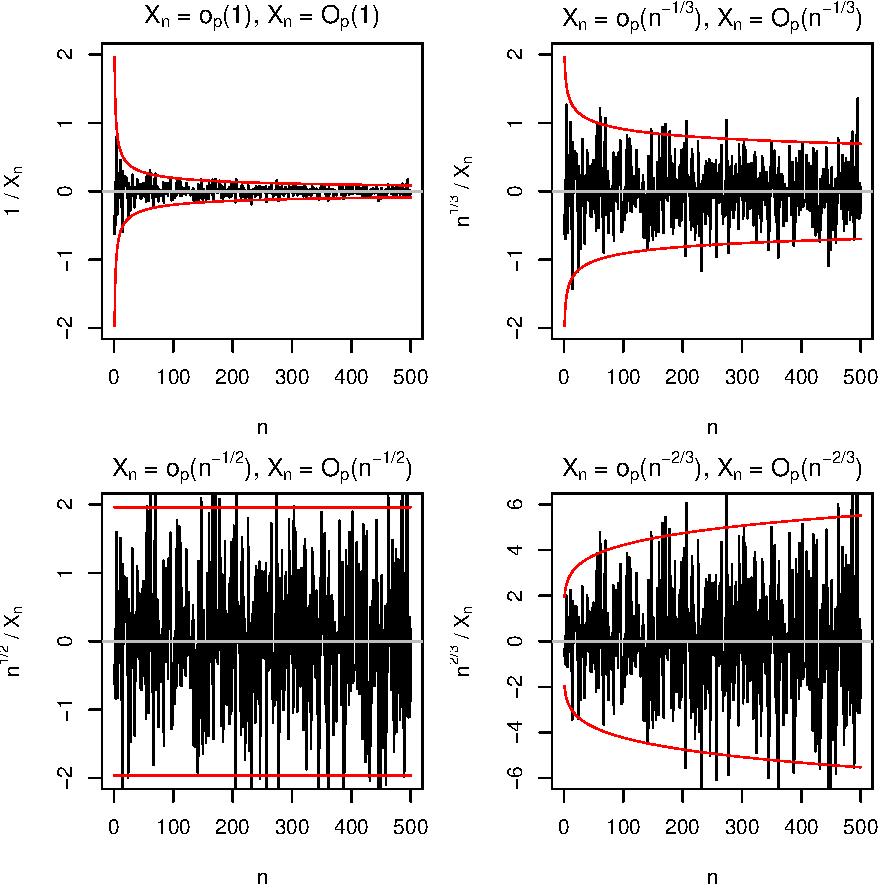
\includegraphics[keepaspectratio]{bigoh_files/figure-pdf/unnamed-chunk-2-1.pdf}}
\end{center}

\begin{exercise}[]\protect\hypertarget{exr-probconvexr}{}\label{exr-probconvexr}

It is actually true that:

\begin{enumerate}
\def\labelenumi{\arabic{enumi}.}
\item
  \(X_n \stackrel{P}{\rightarrow}0\).
\item
  \(n^{1/3}X_n \stackrel{P}{\rightarrow} 0\).
\item
  \(n^{1/2}X_n \stackrel{P}{\rightarrow} \mathcal{N}(0,1)\).
\end{enumerate}

\end{exercise}

다음은 (Jiang 2022) 에 나와있는 정리다.

\begin{theorem}[\(O_p(1)\)이기 위한
충분조건]\protect\hypertarget{thm-suffbigop}{}\label{thm-suffbigop}

다음 세 가지 조건 중 하나를 만족하면 \(X_n = O_p(1)\)이다.

\begin{enumerate}
\def\labelenumi{\arabic{enumi}.}
\item
  There is \(p>0\) such that \(E(|X_n|^p), n\geq 1\) is bounded.
\item
  \(X_n\stackrel{p}{\rightarrow}X\) as \(n\rightarrow\infty\) for some
  random variable \(X\).
\item
  \(X_n \stackrel{d}{\rightarrow}X\) as \(n\rightarrow\infty\) for some
  random variable \(X\). (Polansky (2011) 의 theorem 8.1)
\end{enumerate}

\end{theorem}

\begin{tcolorbox}[enhanced jigsaw, left=2mm, arc=.35mm, leftrule=.75mm, colback=white, title=\textcolor{quarto-callout-note-color}{\faInfo}\hspace{0.5em}{Proof}, rightrule=.15mm, breakable, bottomrule=.15mm, coltitle=black, opacitybacktitle=0.6, opacityback=0, toptitle=1mm, titlerule=0mm, toprule=.15mm, colbacktitle=quarto-callout-note-color!10!white, bottomtitle=1mm, colframe=quarto-callout-note-color-frame]

\begin{itemize}
\item
  1번이 성립한다고 하자. \(\varepsilon>0\)에 대해 Chebyshev 부등식을
  쓰면 \[
  \begin{align*}
  P(|X_n|>M) &= P(|X_n|^p > M^p)\\
  &\leq \frac{E(|X_n|^p)}{M^p} \leq \frac{c}{M^p},
  \end{align*}
  \] where \(c= \sup_{n\geq 1}E(|X_n|^p)<\infty\). Thus, if we choose
  \(M\) such that \(M>(c/\varepsilon)^{1/p}\), we have
  \(P(|X_n|>M)<\varepsilon\). Hence, \(P(|X_n|\leq M) > 1-\varepsilon\)
  for any \(n\geq 1\).
\item
  3번 관련
  \href{https://stats.stackexchange.com/questions/567308/converge-in-distribution-and-order-of-convergence}{StackExchange}
  참고
\end{itemize}

\end{tcolorbox}

다음은 big-\(O_p\) 및 little-\(o_p\)에 관한 성질들이다.

\begin{proposition}[]\protect\hypertarget{prp-bigoplittleop}{}\label{prp-bigoplittleop}

Consider two strictly positive sequences \(a_n, b_n \rightarrow 0\). The
following properties hold (García-Portugués 2024) :

\begin{enumerate}
\def\labelenumi{\arabic{enumi}.}
\item
  \(o_p(a_n) = O_p(a_n)\) (little-\(o_p\) implies big-\(O_p\))
\item
  \(o(1) = o_p(1)\), \(O(1) = O_p(1)\) (deterministic implies
  probabilistic)
\item
  \(kO_p(a_n) = O_p(a_n)\), \(k o_p(a_n) = o_p (a_n), k\in \mathbb{R}\).
\item
  \(o_p(a_n) + o_p(b_n) = o_p(a_n + b_n)\),
  \(O_p(a_n) + O_p(b_n) = O_p(a_n + b_n)\).
\item
  \(o_p(a_n)o_p(b_n) = o_p(a_n b_n)\),
  \(O_p(a_n)O_p(b_n) = O_p(a_n b_n)\) .
\item
  \(o_p(a_n) + O_p(b_n) = O_p(a_n + b_n)\),
  \(o_p(a_n)O_p(b_n)=o_p(a_n b_n)\).
\item
  \(o_p(1) O_p(a_n) = o_p (a_n)\).
\item
  \((1+o_p(1))^{-1} = O_p(1)\).
\end{enumerate}

\end{proposition}

\begin{example}[]\protect\hypertarget{exm-bigop2}{}\label{exm-bigop2}

위 proposition의 2, 4번을 이용하면 Example~\ref{exm-bigop1} 에 다음과
같은 표현이 가능하다. \[
\begin{align*}
X_n &= O(E[X_n]) + O_p (\sqrt{\text{var}[X_n]})\\
&= O_p(E[X_n] + \sqrt{\text{var}[X_n]}).
\end{align*}
\]

\end{example}

Polansky (2011) 의 theorem 8.3에서는 big-O, small-o, big-\(O_p\),
small-\(o_p\)에 대한 모든 곱의 상황을 정리해 놓았다.

\begin{theorem}[]\protect\hypertarget{thm-bigoplittleopinteraction}{}\label{thm-bigoplittleopinteraction}

Let \(\{X_n\}_{n=1}^{\infty}\) and \(\{Y_n \}_{n=1}^{\infty}\) be
sequences of random variables and let \(\{y_n\}_{n=1}^{\infty}\) be a
sequence of real numbers.

\begin{enumerate}
\def\labelenumi{\arabic{enumi}.}
\item
  If \(X_n = O_p (n^{-a})\) and \(Y_n = O_p(n^{-b})\) as
  \(n\rightarrow\infty\), then \(X_n Y_n = O_p(n^{-(a+b)})\) as
  \(n\rightarrow\infty\).
\item
  If \(X_n = O_p (n^{-a})\) and \(Y_n = o(n^{-b})\) as
  \(n\rightarrow\infty\), then \(X_n y_n = o_p(n^{-(a+b)})\) as
  \(n\rightarrow\infty\).
\item
  If \(X_n = O_p (n^{-a})\) and \(Y_n = o_p(n^{-b})\) as
  \(n\rightarrow\infty\), then \(X_n Y_n = o_p(n^{-(a+b)})\) as
  \(n\rightarrow\infty\).
\item
  If \(X_n = o_p (n^{-a})\) and \(y_n = o(n^{-b})\) as
  \(n\rightarrow\infty\), then \(X_n y_n = o_p(n^{-(a+b)})\) as
  \(n\rightarrow\infty\).
\item
  If \(X_n = O_p (n^{-a})\) and \(y_n = O(n^{-b})\) as
  \(n\rightarrow\infty\), then \(X_n y_n = O_p(n^{-(a+b)})\) as
  \(n\rightarrow\infty\).
\item
  If \(X_n = o_p (n^{-a})\) and \(y_n = O(n^{-b})\) as
  \(n\rightarrow\infty\), then \(X_n y_n = o_p(n^{-(a+b)})\) as
  \(n\rightarrow\infty\).
\item
  If \(X_n = o_p (n^{-a})\) and \(Y_n = o_p(n^{-b})\) as
  \(n\rightarrow\infty\), then \(X_n Y_n = o_p(n^{-(a+b)})\) as
  \(n\rightarrow\infty\).
\end{enumerate}

\end{theorem}

다음은 \href{https://www.sfu.ca/~lockhart/richard/830/20_3/}{Richard
Lockhart 교수님의 강의노트} 나 Shumway and Stoffer (2017) 의 appendix
A에서 알 수 있는 big-O, small-o, big-\(O_p\), small-\(o_p\) 덧셈 관련
내용이다.

\begin{theorem}[]\protect\hypertarget{thm-bigoplittleopaddition}{}\label{thm-bigoplittleopaddition}

\(a_n>0\), \(b_n>0\)

\begin{enumerate}
\def\labelenumi{\arabic{enumi}.}
\item
  \(O(a_n) + O(b_n) = O(\max \{a_n ,b_n\})\)
\item
  \(o(a_n) + o(b_n) = o(\max \{a_n ,b_n\})\)
\item
  \(O_p(a_n) + O_p(b_n) = O_p(\max \{a_n ,b_n\})\)
\item
  \(o_p(a_n) + o_p(b_n) = o_p(\max \{a_n ,b_n\})\)
\item
  \(o(O(a_n)) = o(a_n)\)
\item
  \(o(a_n) + O(b_n) = O(\max \{a_n ,b_n\})\)
\item
  \(o_p(a_n) + O_p(b_n) = O_p(\max \{a_n ,b_n\})\)
\end{enumerate}

You can't cancel because each new occurence of \(O\) is different \[
O(a_n) - O(a_n) \neq 0,
\] only add and multiply and use positive rates.

\end{theorem}

\chapter*{Summary}\label{summary}
\addcontentsline{toc}{chapter}{Summary}

\markboth{Summary}{Summary}

In summary, this book has no content whatsoever.

\begin{Shaded}
\begin{Highlighting}[]
\DecValTok{1} \SpecialCharTok{+} \DecValTok{1}
\end{Highlighting}
\end{Shaded}

\begin{verbatim}
[1] 2
\end{verbatim}

\chapter*{References}\label{references-1}
\addcontentsline{toc}{chapter}{References}

\markboth{References}{References}

\phantomsection\label{refs}
\begin{CSLReferences}{1}{0}
\bibitem[\citeproctext]{ref-Durrett2019}
Durrett, Rick. 2019. \emph{Probability: Theory and Examples}. 5th ed.
Cambridge University Press.
\url{https://www.ebook.de/de/product/34699864/rick_duke_university_north_carolina_durrett_probability.html}.

\bibitem[\citeproctext]{ref-Garcia-Portugues2024}
García-Portugués, E. 2024. \emph{Notes for Nonparametric Statistics}.
\url{https://bookdown.org/egarpor/NP-UC3M/}.

\bibitem[\citeproctext]{ref-Gut2014}
Gut, Allan. 2014. \emph{Probability: A Graduate Course}. 2nd ed.
Springer New York.

\bibitem[\citeproctext]{ref-Haigh2013}
Haigh, John. 2013. \emph{Probability Models}. 2nd ed. 2013.
SpringerLink. Dordrecht: Springer.

\bibitem[\citeproctext]{ref-Hansen2022}
Hansen, Bruce. 2022. \emph{Econometrics}. Princeton University Press.

\bibitem[\citeproctext]{ref-Jiang2022}
Jiang, Jiming. 2022. \emph{Large Sample Techniques for Statistics}.
\emph{Springer Texts in Statistics}. Springer International Publishing.
\url{https://doi.org/10.1007/978-3-030-91695-4}.

\bibitem[\citeproctext]{ref-Nolan2020}
Nolan, John P. 2020. \emph{Univariate Stable Distributions: Models for
Heavy Tailed Data}. Springer Series in Operations Research and Financial
Engineering. Cham, Switzerland: Springer.

\bibitem[\citeproctext]{ref-Polansky2011}
Polansky, Alan M. 2011. \emph{Introduction to Statistical Limit Theory}.
CRC Press.

\bibitem[\citeproctext]{ref-Proschan2016}
Proschan, Michael A. 2016. \emph{Essentials of Probability Theory for
Statisticians}. CRC Press.

\bibitem[\citeproctext]{ref-Shumway2017}
Shumway, Robert H., and David S. Stoffer. 2017. \emph{Time Series
Analysis and Its Applications}. Springer-Verlag GmbH.
\url{https://www.ebook.de/de/product/28224354/robert_h_shumway_david_s_stoffer_time_series_analysis_and_its_applications.html}.

\end{CSLReferences}




\end{document}
